%%%%%%%%%%%%%%%%%%%%%%%%%%%%%%%%%%%%%%%%%%%%%%%%%%%%%%%%%%%%%%%%%%%%%%%%%%%%%%%%
%% LaTeX sources for The Guide to Functional Programming
%% Michael B. Gale (m.gale@warwick.ac.uk)
%%
%% This work is licensed under the Creative Commons
%% Attribution-NonCommercial-ShareAlike 2.0 UK: England & Wales License. To
%% view a copy of this license, visit
%% http://creativecommons.org/licenses/by-nc-sa/2.0/uk/ or send a letter to
%% Creative Commons, PO Box 1866, Mountain View, CA 94042, USA.
%%%%%%%%%%%%%%%%%%%%%%%%%%%%%%%%%%%%%%%%%%%%%%%%%%%%%%%%%%%%%%%%%%%%%%%%%%%%%%%%

\documentclass[12pt,a4paper,twoside,fleqn]{report}

\usepackage{geometry}
\usepackage[latin1]{inputenc}
\usepackage{amsmath}
\usepackage{amsfonts}
\usepackage{amssymb}
\usepackage{graphicx}
\usepackage{fancyeq}
\usepackage{fancyhdr}
\usepackage[explicit]{titlesec}
\usepackage{color}
\usepackage{longtable}
\usepackage{array, booktabs}
\usepackage{colortbl}
\usepackage{wrapfig}
\usepackage{pgfplots}
\usepackage[strict]{changepage}
\usepackage{graphbox}
\usepackage{prerex}
\usepackage{forest}
\usepackage{multicol}
\usepackage{fontawesome}
\usepackage{natbib}

% Minted -------------------------------

\usepackage{minted}
\usepackage[
backgroundcolor = gray!5
, hidealllines=true
]{mdframed}

\surroundwithmdframed{minted}
\usemintedstyle{lovelace}

\setminted[text]{fontsize=\small}
\setminted[haskell]{fontsize=\small}
\setminted[bash]{fontsize=\small}
\newcommand{\haskellIn}[1]{\mintinline[fontsize=\small]{haskell}{#1}}
\newcommand{\bashIn}[1]{\mintinline[fontsize=\small]{bash}{#1}}

% Tikz -------------------------------

\usepackage{tikz}
\usetikzlibrary{arrows}

\tikzset{
	treenode/.style = {align=center, inner sep=0pt, text centered,
		font=\sffamily},
	arn_n/.style = {treenode, circle, white, font=\sffamily\bfseries, draw=black,
		fill=black, text width=1.5em},
	arn_r/.style = {treenode, circle, red, draw=red,
		text width=1.5em, very thick},
	arn_x/.style = {treenode, circle, draw=white,
		minimum width=1.5em, minimum height=1.5em},
	cls/.style = { treenode, rectangle, red, draw=red,
		text width=1.5em, very thick, minimum width=1.5em, minimum height=1.5em }
}

% UK English -------------------------------
\usepackage[UKenglish]{babel}
\usepackage[UKenglish]{isodate}

% Hyperref -------------------------------
\usepackage{hyperref}
\hypersetup{
    colorlinks=true,
    linkcolor=black,
    urlcolor=black,
    citecolor=black,
    unicode=false
}

% cleveref
\usepackage[nameinlink]{cleveref}

\crefname{figure}{figure}{figures} % cleveref by default has `fig.'
\Crefname{figure}{Figure}{Figures}

\crefname{section}{section}{sections} % cleveref by default has `fig.'
\Crefname{section}{Section}{Sections}

% Fonts -------------------------------
\usepackage[]{FiraSans}

% Palatino (font)
\usepackage{mathpazo}
\linespread{1.05}         % Palatino needs more leading (space between lines)
\usepackage[T1]{fontenc}

% some format settings
% for hard-bound final submission, use:
%\setlength{\oddsidemargin}{4.6mm}     % 30 mm left margin - 1 in
% for soft-bound version and techreport, use instead:
\setlength{\oddsidemargin}{-0.4mm}    % 25 mm left margin - 1 in
\setlength{\evensidemargin}{-0.4mm}
\setlength{\topmargin}{-5.4mm}        % 20 mm top margin - 1 in
\setlength{\textwidth}{160mm}         % 20/25 mm right margin
\setlength{\textheight}{237mm}        % 20 mm bottom margin
\setlength{\headheight}{5mm}
\setlength{\headsep}{5mm}
\setlength{\parindent}{0mm}
\setlength{\parskip}{\medskipamount}
\renewcommand\baselinestretch{1.2} % thesis format (not needed for techreport)
% don't let large figures hijack entire pages
\renewcommand\topfraction{.9}
\renewcommand\textfraction{.1}
\renewcommand\floatpagefraction{.8}

\usepackage[nomap]{FiraMono}

\usepackage{microtype}
\DisableLigatures[f]{encoding = *, family = tt* }

\author{Michael B. Gale}


\definecolor{gray75}{gray}{0.75}
\newcommand{\hsp}{\hspace{20pt}}

\titleformat{name=\chapter}[hang]{}{}{0cm}{%
	\protect\thispagestyle{fancy}
	\begin{center}
		\large $\lambda$.\thechapter \\
		\huge \textsc{#1}
	\end{center}
	%\chaptermark{\chapter}
}
\titleformat{name=\chapter,numberless}[hang]{}{}{0cm}{%
	\begin{center}
		\huge \textsc{#1}
	\end{center}
	%\chaptermark{\chapter}
}

%\titleformat{\subsection}{format}{label}{0em}{before-code}

\titleformat{\section}
	{\bfseries\large}
	{\llap{\parbox{1.5cm}{\thesection\hfill}}#1}
	{0em}
	{\bfseries}

\titleformat{\subsection}
{\bfseries}{\llap{\parbox{1.5cm}{\thesubsection\hfill}}#1}{0em}{\bfseries}


% misc. commands
\newcounter{TaskCounter}

\newcommand{\question}[1]{\vspace{-0.7cm}{\footnotesize \emph{#1}} \vspace{0.25cm}}
\newcommand{\topics}[1]{\vspace{-0.5cm}{\footnotesize \emph{Topics}: #1} \vspace{0.25cm}}
\newcommand{\task}[2][]{\indent\llap{\parbox{1.5cm}{\refstepcounter{TaskCounter}\label{#1}{\firamedium Ex\theTaskCounter}\hfill}}#2}
\newcommand{\solution}[2]{\indent\llap{\parbox{1.5cm}{\textbf{Ex#1}\hfill}}#2}
\newcommand{\taskLine}{\bigskip\hrule\bigskip}



% titles, dates, etc. of lectures and labs

% lecture 1
\newcommand{\lectureOneTitle}{Introduction}
\newcommand{\lectureOneDate}{7 January}
\newcommand{\lectureOneQuestion}{What is functional programming and why should we learn it?}
\newcommand{\lectureOneTopics}{Overview of programming paradigms \& models of computation, examples of applications of functional programming, module overview, and recommended texts.}

% lecture 2
\newcommand{\lectureTwoTitle}{Definitions \& functions}
\newcommand{\lectureTwoDate}{8 January}
\newcommand{\lectureTwoQuestion}{How do we write simple programs in Haskell?}
\newcommand{\lectureTwoTopics}{Definitions, basic arithmetic expressions, string values, boolean values, functions, using built-in functions, and basic pattern matching.}

% lecture 3
\newcommand{\lectureThreeTitle}{Basic types}
\newcommand{\lectureThreeDate}{9 January}
\newcommand{\lectureThreeQuestion}{How does the compiler prevent us from writing bad software?}
\newcommand{\lectureThreeTopics}{Basic types, function types, parametric polymorphism, lists, and pairs.}

% lecture 3b
\newcommand{\lectureThreeBTitle}{Lists}
\newcommand{\lectureThreeBDate}{14 January}
\newcommand{\lectureThreeBQuestion}{How do we use lists in Haskell?}
\newcommand{\lectureThreeBTopics}{Constructing lists, pattern-matching on lists, and list comprehensions.}

% lecture 4
\newcommand{\lectureFourTitle}{Type classes}
\newcommand{\lectureFourDate}{15 January}
\newcommand{\lectureFourQuestion}{How can we restrict polymorphism and overload functions?}
\newcommand{\lectureFourTopics}{Ad-hoc polymorphism via type classes, built-in type classes, and type class constraints.}

% lecture 5
\newcommand{\lectureFiveTitle}{Recursive functions}
\newcommand{\lectureFiveDate}{16 January}
\newcommand{\lectureFiveQuestion}{How do we express loops without mutable state?}
\newcommand{\lectureFiveTopics}{Writing recursive functions for basic types (numbers, lists/strings), defining built-in functions ourselves.}

% lecture 6
\newcommand{\lectureSixTitle}{Higher-order functions}
\newcommand{\lectureSixDate}{21 January}
\newcommand{\lectureSixQuestion}{Can we write functions which abstract over common behaviours?}
\newcommand{\lectureSixTopics}{Higher-order functions such as \haskellIn{map}, \haskellIn{filter}, etc., recursion primitives such as \haskellIn{foldr} and \haskellIn{foldl}.}

% lecture 7
\newcommand{\lectureSevenTitle}{Data types \& type aliases}
\newcommand{\lectureSevenDate}{22 January}
\newcommand{\lectureSevenQuestion}{How can we define our own types in Haskell?}
\newcommand{\lectureSevenTopics}{Type aliases, data types, data constructors, pattern matching on custom data constructors, recursion on values of custom types.}

% lecture 8
\newcommand{\lectureEightTitle}{Coursework I briefing}
\newcommand{\lectureEightDate}{23 January}
\newcommand{\lectureEightQuestion}{What is the first coursework about?}
\newcommand{\lectureEightTopics}{Demonstration of what the completed coursework will do, five-guess algorithm, introduction to the skeleton code.}

% lecture 9
\newcommand{\lectureNineTitle}{Lazy evaluation}
\newcommand{\lectureNineDate}{28 January}
\newcommand{\lectureNineQuestion}{What order are programs evaluated in?}
\newcommand{\lectureNineTopics}{Strict and lazy evaluation, calling conventions, benefits and disadvantages, and examples of lazy evaluation.}

% lecture 9b
\newcommand{\lectureNineBTitle}{\emph{Fun with} testing}
\newcommand{\lectureNineBDate}{29 January}
\newcommand{\lectureNineBQuestion}{What tools are there for testing and how do we use them?}
\newcommand{\lectureNineBTopics}{Unit testing and property-based testing in Haskell.}

% lecture 10
\newcommand{\lectureTenTitle}{Reasoning about programs}
\newcommand{\lectureTenDate}{30 January}
\newcommand{\lectureTenQuestion}{Can we use formal reasoning techniques to prove properties about our programs?}
\newcommand{\lectureTenTopics}{Equational reasoning, proofs by induction.}

% lecture 11
\newcommand{\lectureElevenTitle}{Reasoning about programs (cont.)}
\newcommand{\lectureElevenDate}{4 February}
\newcommand{\lectureElevenQuestion}{Can we use formal reasoning techniques to prove properties about our programs?}
\newcommand{\lectureElevenTopics}{Equational reasoning, proofs by induction.}

% lecture 11b
\newcommand{\lectureElevenBTitle}{\emph{Fun with} constructive induction}
\newcommand{\lectureElevenBDate}{5 February}
\newcommand{\lectureElevenBQuestion}{Can we use formal reasoning techniques to calculate more efficient programs?}
\newcommand{\lectureElevenBTopics}{Constructive induction.}

% lecture 12
\newcommand{\lectureTwelveTitle}{Functors \& applicative functors}
\newcommand{\lectureTwelveDate}{6 February}
\newcommand{\lectureTwelveQuestion}{Are there any useful design patterns in functional programming?}
\newcommand{\lectureTwelveTopics}{Functors, applicative functions, applications of applicative functors.}

% lecture 12b
\newcommand{\lectureTwelveBTitle}{Functors \& applicative functors (cont.)}
\newcommand{\lectureTwelveBDate}{11 February}
\newcommand{\lectureTwelveBQuestion}{Are there any useful design patterns in functional programming?}
\newcommand{\lectureTwelveBTopics}{Functors, applicative functions, applications of applicative functors.}

% lecture 12c
\newcommand{\lectureTwelveCTitle}{\emph{Fun with} applicative functors}
\newcommand{\lectureTwelveCDate}{12 February}
\newcommand{\lectureTwelveCQuestion}{What can we do with applicative functors?}
\newcommand{\lectureTwelveCTopics}{Applicative functors in action.}

% lecture 12d
\newcommand{\lectureTwelveDTitle}{Coursework II briefing}
\newcommand{\lectureTwelveDDate}{13 February}
\newcommand{\lectureTwelveDQuestion}{What is the second coursework about?}
\newcommand{\lectureTwelveDTopics}{Demonstration of what the completed coursework will do, semantics of the programming language, introduction to the skeleton code.}

% lecture 13
\newcommand{\lectureThirteenTitle}{Foldables}
\newcommand{\lectureThirteenDate}{18 February}
\newcommand{\lectureThirteenQuestion}{Are there any other useful design patterns in functional programming?}
\newcommand{\lectureThirteenTopics}{\haskellIn{Foldable} type class, its motivation, and examples.}

% lecture 14
\newcommand{\lectureFourteenTitle}{Sequential composition}
\newcommand{\lectureFourteenDate}{19 February}
\newcommand{\lectureFourteenQuestion}{How do structure programs in which one part of a program relies on the result of another part?}
\newcommand{\lectureFourteenTopics}{Some functions for the sequential composition of \texttt{\small Maybe} values.}

% lecture 15
\newcommand{\lectureFifteenTitle}{Sequential composition (cont.)}
\newcommand{\lectureFifteenDate}{25 February}
\newcommand{\lectureFifteenQuestion}{Are there other examples of sequential composition?}
\newcommand{\lectureFifteenTopics}{Some functions for the sequential composition of \texttt{\small State} values and some laws for sequential composition.}

% lecture 16
\newcommand{\lectureSixteenTitle}{\emph{Fun with} sequential composition}
\newcommand{\lectureSixteenDate}{26 February}
\newcommand{\lectureSixteenQuestion}{How is sequential composition used in practice?}
\newcommand{\lectureSixteenTopics}{Sequential composition in action.}

% lecture 17
\newcommand{\lectureSeventeenTitle}{Input and output}
\newcommand{\lectureSeventeenDate}{27 February}
\newcommand{\lectureSeventeenQuestion}{Can we write impure programs in a pure programming language?}
\newcommand{\lectureSeventeenTopics}{The \texttt{\small IO} monad.}

% lecture 18
\newcommand{\lectureEighteenTitle}{Type promotion \& GADTs}
\newcommand{\lectureEighteenDate}{4 March}
\newcommand{\lectureEighteenQuestion}{How can we encode more information in types?}
\newcommand{\lectureEighteenTopics}{Phantom types, GADTs, singleton types, pattern matching with GADTs.}

% lecture 18b
\newcommand{\lectureEighteenBTitle}{\emph{Fun with} IO}
\newcommand{\lectureEighteenBDate}{5 March}
\newcommand{\lectureEighteenBQuestion}{What do Haskell programs that make use of IO look like?}
\newcommand{\lectureEighteenBTopics}{The \texttt{\small IO} monad in action.}

% lecture 19
\newcommand{\lectureNineteenTitle}{Type families}
\newcommand{\lectureNineteenDate}{6 March}
\newcommand{\lectureNineteenQuestion}{How can we perform computation at the type-level?}
\newcommand{\lectureNineteenTopics}{Closed and open type families.}

% lecture 20
\newcommand{\lectureTwentyTitle}{Type-level programming}
\newcommand{\lectureTwentyDate}{11 March}
\newcommand{\lectureTwentyQuestion}{How do we make type-level programming practical in Haskell?}
\newcommand{\lectureTwentyTopics}{Singletons, proxies, and reification.}

% lecture 21
\newcommand{\lectureTwentyOneTitle}{\emph{Fun with} type-level programming}
\newcommand{\lectureTwentyOneDate}{12 March}
\newcommand{\lectureTwentyOneQuestion}{What are some examples of how type-level programming is used?}
\newcommand{\lectureTwentyOneTopics}{Type-level programming in action.}

% lecture 22
\newcommand{\lectureTwentyTwoTitle}{Conclusions}
\newcommand{\lectureTwentyTwoDate}{13 March}
\newcommand{\lectureTwentyTwoQuestion}{What have we learnt about functional programming?}
\newcommand{\lectureTwentyTwoTopics}{Summary of the module, information about the exam, and other general information.}

% practical 1
\newcommand{\practicalOneTitle}{Getting started}
\newcommand{\practicalOneDate}{7-11 January}
\newcommand{\practicalOneAims}{You will learn how to use some of the tools that we will be using as part of this module.}

% practical 2
\newcommand{\practicalTwoTitle}{Types \& list comprehensions}
\newcommand{\practicalTwoDate}{14-18 January}
\newcommand{\practicalTwoAims}{This lab teaches you to understand type errors and how to fix them. You will also learn about list comprehensions.}

% practical 3
\newcommand{\practicalThreeTitle}{Recursive \& higher-order functions}
\newcommand{\practicalThreeDate}{21-25 January}
\newcommand{\practicalThreeAims}{By the end of this lab, you should be able to solve problems by writing recursive and higher-order functions.}

% practical 4
\newcommand{\practicalFourTitle}{User-defined types}
\newcommand{\practicalFourDate}{\parbox{2.2cm}{28 January-\linebreak 1 February}}
\newcommand{\practicalFourAims}{You will define your own types and functions which work with them.}

% practical 5
\newcommand{\practicalFiveTitle}{Lazy evaluation and equational reasoning}
\newcommand{\practicalFiveDate}{4-8 February}
\newcommand{\practicalFiveAims}{The goal of this lab is for you to be able to write programs which make effective use of lazy evaluation, such as for backtracking or infinite data. You will also prove some properties about your programs using equational reasoning and structural induction.}

% practical 6
\newcommand{\practicalSixTitle}{Functors}
\newcommand{\practicalSixDate}{11-15 February}
\newcommand{\practicalSixAims}{You will write programs using functors.}

% practical 6b
\newcommand{\practicalSixBTitle}{Applicative functors}
\newcommand{\practicalSixBDate}{18-22 February}
\newcommand{\practicalSixBAims}{You will write programs using applicative functors.}

% practical 7
\newcommand{\practicalSevenTitle}{Foldables}
\newcommand{\practicalSevenDate}{\parbox{2.4cm}{25 February-\linebreak 1 March}}
\newcommand{\practicalSevenAims}{In this lab, you will write programs using foldables.}

% practical 8
\newcommand{\practicalEightTitle}{Effectful programs}
\newcommand{\practicalEightDate}{4-8 March}
\newcommand{\practicalEightAims}{You will write programs using monads, define your own instances of the \haskellIn{Monad} type class, and reason about monad laws.}

% practical 9
\newcommand{\practicalNineTitle}{Type-level programming}
\newcommand{\practicalNineDate}{11-15 March}
\newcommand{\practicalNineAims}{You should be able to write simple programs at the type-level using GADTs and type families.}

\AtBeginDocument{\addtocontents{toc}{\protect\thispagestyle{fancy}}}

\begin{document}
\fancypagestyle{empty}{\fancyhf{}}
\pagestyle{empty}
\pagenumbering{roman} 

\renewcommand{\headrulewidth}{0pt}
\renewcommand{\footrulewidth}{0pt}

%%%%%%%%%%%%%%%%%%%%%%%%%%%%%%%%%%%%%%%%%%%%%%%%%%%%%%%%%%%%%%%%%%%%%%%%%%%%%%%%
%% LaTeX sources for The Guide to Functional Programming
%% Michael B. Gale (m.gale@warwick.ac.uk)
%%
%% This work is licensed under the Creative Commons
%% Attribution-NonCommercial-ShareAlike 2.0 UK: England & Wales License. To
%% view a copy of this license, visit
%% http://creativecommons.org/licenses/by-nc-sa/2.0/uk/ or send a letter to
%% Creative Commons, PO Box 1866, Mountain View, CA 94042, USA.
%%%%%%%%%%%%%%%%%%%%%%%%%%%%%%%%%%%%%%%%%%%%%%%%%%%%%%%%%%%%%%%%%%%%%%%%%%%%%%%%

\begin{titlepage}
	\begin{center}
		
{\Huge \textit{The guide to}} \\[0.2cm]
{\Huge \textbf{Functional Programming}} \\[0.2cm]

\vfill

\scalebox{25.0}{$\lambda$}

\vfill 

{\LARGE Michael B. Gale} \\[0.1cm]
{\large \href{mailto:m.gale@warwick.ac.uk}{m.gale@warwick.ac.uk}}

\vspace{1cm}

{\Large 2020/21}
\end{center}
\end{titlepage}

\phantom{~}
\vfill

\ccbyncnd

\vspace*{0.2cm}

This work is licensed under a Creative Commons Attribution-NonCommercial-NoDerivatives 4.0 International License. 

\vspace*{0.2cm}

\url{http://creativecommons.org/licenses/by-nc-nd/4.0/}


\cleardoublepage
%\setcounter{page}{1}

\fancyhf{}
\fancyhead[LE, RO]{\emph{Functional Programming (CS141)}}
\fancyhead[LO, RE]{\emph{Michael B. Gale}}
%\fancyhead[RE,LO]{Guides and tutorials}
%\fancyfoot[CE,CO]{\leftmark}
\fancyfoot[LE,RO]{\thepage}
\pagestyle{fancy}
\thispagestyle{fancy}
\newgeometry{
	tmargin=2.5cm,
	textwidth=155mm, 
	textheight=247mm,
	headheight=5mm,
	headsep=5mm,
	inner=30mm
}

\tableofcontents


\cleardoublepage
\pagenumbering{arabic}

\chapter{Overview}

\emph{Functional Programming} is an optional module which follows on from modules such as CS118, CS132, or equivalents in other departments where you have learnt to write programs in the imperative style in languages such as C and Java. However, C and Java are just two of many programming languages and object-oriented programming is just one of many programming paradigms. You may think of programming languages as tools: a hammer is different from a screwdriver and both serve different purposes which they are good at. Programming languages are the same: different languages exist for different purposes and it is easier or harder to accomplish certain tasks in one or the other. To be a good programmer, you need to know which tools are at your disposal and when to use them.

In this module, you will learn about the functional programming paradigm. No prior programming knowledge is required and this module is suitable for most scientists. We will use Haskell, which is a lazy, purely functional programming language. Writing programs in Haskell is very different than writing programs in languages like Java and over the course of this module you will learn how to do that. In turn, this adds a powerful tool to your programming arsenal, you will gain a much deeper understanding of programming, and skills from this module can be applied in other languages, functional or not. In other words, you will become a better programmer!

This document serves as a companion to the module by giving you an overview of all the major components, including guidance on how to use the different tools you will encounter as part of this module. You can also find the coursework specifications as well as exercises for all of the labs in this guide.
\section{Books}

You are not required to purchase any books for this module as there are many resources available online, including a number of free books. For those of you who prefer to have a book with most of the content in one place, I can recommend the following, all of which are introductory texts. Each book which is recommended here teaches functional programming in a different way\footnote{This reading list is also available on the library website at \url{https://warwick.rl.talis.com/modules/cs141.html} which lets you find copies in the library.}:

\subsubsection{Learn you a Haskell for Great Good!} \vspace{-0.5cm}
\emph{Miran Lipova\v{c}a}, No Starch Press. 

This book is also a general introduction to Haskell with a greater emphasis on concepts in functional programming. If you prefer to learn by focusing on theory and concepts which you can then later apply to problems when you encounter them, this book is for you. It is also available for free on the book's website at:
\begin{center}
	\url{http://learnyouahaskell.com/}
\end{center} 

\subsubsection{Programming in Haskell (2nd edition)} \vspace{-0.5cm}
\emph{Graham Hutton}, Cambridge University Press. 

A general introduction to Haskell which is well-structured and covers all of the major topics from the lectures in a vaguely similar order. This is the ``main text'' and this guide includes references to chapters in Hutton's book for further reading. Note: if you are thinking of buying the first edition, which is likely cheaper at this point, it doesn't cover the later, more advanced topics of this module.

\subsubsection{Real World Haskell} \vspace{-0.5cm}
\emph{Bryan O'Sullivan, Don Stewart, and John Goerzen}, O'Reilly.

This book focuses heavily on solving practical tasks using Haskell after only a brief introduction to the basic concepts. This book is for you if you prefer to learn by seeing how particular techniques are used in action. This book is quite old now, so some of the libraries and techniques used in the book may be outdated by now, but the book is also available for free on the book's website at:
\begin{center}
	\url{http://book.realworldhaskell.org/}
\end{center} 

\subsubsection{The Haskell School of Expression} \vspace{-0.5cm}
\emph{Paul Hudak}, Cambridge University Press.

This book teaches functional programming graphically at the start and later through music. If you like visual and auditory results while you are learning, this book may be for you. Like Real World Haskell, this book is slightly older and some of the code shown may not work without modifications.

\subsubsection{Introduction to Functional Programming} \vspace{-0.5cm}
\emph{Richard Bird and Philip Wadler}, Prentice Hall.

This is an excellent, but old, introduction to functional programming. This book came out before I was born and uses a Haskell precursor language called Miranda. However, it does a very good job at teaching the foundations of functional programming.
\section{Timeline}
\label{sec:timeline}

This module is comprised of approximately 30 lectures, 10 labs, 2 pieces of coursework, and an exam. This section contains a chronological schedule of all of these components. Note that the schedule may be subject to changes due to \emph{e.g.} staff illness or other unforeseen circumstances. Each lecture aims to answer a specific question, which is shown in the timeline. You can test your understanding by asking yourself that question after each lecture and checking that you can answer it. 

There are typically three lectures per week. The definite timetable is available from the timetabling website\footnote{\url{https://timetablingmanagement.warwick.ac.uk/sws1920/}}, on the module website, or you can view your personal timetable on Tabula as well. 

\newcommand{\foo}{\makebox[0pt]{\textbullet}\hskip-0.5pt\vrule width 1pt\hspace{\labelsep}}

\newcommand{\LectureEntry}[4]{#1 & \begin{tabular}{p{11cm}}
		\textbf{#2} \\
		\emph{#3} \\
		#4
\end{tabular}}
\newcommand{\LabEntry}[3]{#1 & \begin{tabular}{p{11cm}}
		\textbf{#2} \\
		#3
\end{tabular}}

\begingroup
%\begin{table}
\newcommand{\oldarraystrech}{\arraystretch}
	\renewcommand\arraystretch{1.4}\vskip-1.5ex
	\begin{longtable}{@{\,}r <{\hskip 2pt} !{\foo} >{\raggedright\arraybackslash}p{12cm}}
		\addlinespace[1.5ex]
		\LabEntry{6-10 January}{Week 1 exercises}{Relevant exercises for this week are \emph{Getting started}, \emph{Basic types}, \emph{Functions}, \emph{Pattern matching}.} \\
		\LectureEntry{6 January}{Lecture 1: Introduction}{What is functional programming and why should we learn it?}{Overview of programming paradigms \& models of computation, examples of applications of functional programming, module overview, and recommended texts.} \\
		\LectureEntry{7 January}{Lecture 2: Definitions \& functions}{How do we write simple programs in Haskell?}{Definitions, basic arithmetic expressions, string values, boolean values, functions, using built-in functions, and basic pattern matching.} \\
		\LectureEntry{8 January}{Lecture 3: Basic types}{How does the compiler prevent us from writing bad software?}{Basic types, function types, parametric polymorphism, lists, and pairs.} \\
		
		\LabEntry{13-17 January}{Week 2 exercises}{Relevant exercises for this week are \emph{Using the standard library}, \emph{Lists}, \emph{List comprehensions}, \emph{Recursive functions}, \emph{Higher-order functions}.} \\
		\LectureEntry{13 January}{Lecture 4: Lists}{How do we use lists in Haskell?}{Constructing lists, pattern-matching on lists, and list comprehensions.} \\
		\LectureEntry{14 January}{Lecture 5: Recursive functions}{How do we express loops without mutable state?}{Writing recursive functions for basic types (numbers, lists/strings), defining built-in functions ourselves.} \\
		\LectureEntry{15 January}{Lecture 6: Higher-order functions}{Can we write functions which abstract over common behaviours?}{Higher-order functions such as \haskellIn{map}, \haskellIn{filter}, etc., recursion primitives such as \haskellIn{foldr} and \haskellIn{foldl}.} \\
		
		\LabEntry{20-24 January}{Week 3 exercises}{Relevant exercises for this week are \emph{Data types}, \emph{Type aliases}, and \emph{Using general libraries}.} \\
		\LectureEntry{20 January}{Lecture 7: Data types \& type aliases}{How can we define our own types in Haskell?}{Type aliases, data types, data constructors, pattern matching on custom data constructors, recursion on values of custom types.} \\
		\LectureEntry{21 January}{Lecture 8: \emph{Fun with} functions}{What are some more examples of functions?}{Extended examples of using and defining functions.} \\
		\LectureEntry{22 January}{Lecture 9: Coursework I briefing}{What is the first coursework about?}{Demonstration of what the completed coursework will do, explanation of the rules, introduction to the skeleton code.} \\
		
		\LabEntry{27-31 January}{Week 4 exercises}{Relevant exercises for this week are \emph{Type classes}.} \\
		\LectureEntry{27 January}{Lecture 10: Type classes}{How can we restrict polymorphism and overload functions?}{Ad-hoc polymorphism via type classes, built-in type classes, and type class constraints.} \\
		\LectureEntry{28 January}{Lecture 11: \emph{Fun with} type classes}{How are type classes used in Haskell?}{Examples of type class and their instances.} \\
		\LectureEntry{29 January}{Lecture 12: Testing}{What tools are there for testing and how do we use them?}{Unit testing, property-based testing, and code coverage in Haskell.} \\
		
		\LabEntry{3-7 February}{Week 5 exercises}{Recommended exercises for this week are \emph{Proofs}.} \\
		\LectureEntry{3 February}{Lecture 13: Reasoning about programs}{Can we use formal reasoning techniques to prove properties about our programs?}{Equational reasoning, proofs by induction.} \\
		\LectureEntry{4 February}{Lecture 14: Reasoning about programs (cont.)}{Can we use formal reasoning techniques to prove properties about our programs?}{Equational reasoning, proofs by induction.} \\
		\LectureEntry{5 February}{Lecture 15: Constructive induction}{Can we use formal reasoning techniques to calculate more efficient programs?}{Using induction to calculate faster functions.} \\
		
		\hline
		6 February & \begin{tabular}{p{13cm}}
			\textbf{Deadline: Coursework I} 
		\end{tabular}\\
		\hline
		
		\LabEntry{10-14 February}{Week 6 exercises}{Relevant exercises for this week are \emph{Lazy evaluation}, \emph{Foldables}, and \emph{Functors}.} \\
		\LectureEntry{10 February}{Lecture 16: Lazy evaluation}{What order are programs evaluated in?}{Strict and lazy evaluation, calling conventions, benefits and disadvantages, and examples of lazy evaluation.} \\
		\LectureEntry{11 February}{Lecture 17: Foldables}{Are there any useful design patterns in functional programming?}{\haskellIn{Foldable} type class, its motivation, and examples.} \\
		\LectureEntry{12 February}{Lecture 18: Functors \& applicative functors}{Are there any other useful design patterns in functional programming?}{Functors, applicative functions, applications of applicative functors.} \\
		
		\LabEntry{17-21 February}{Week 7 exercises}{Relevant exercises for this week are \emph{Applicatives}.} \\
		\LectureEntry{17 February}{Lecture 19: Functors \& applicative functors (cont.)}{Are there any other useful design patterns in functional programming?}{Functors, applicative functions, applications of applicative functors.} \\
		\LectureEntry{18 February}{Lecture 20: \emph{Fun with} applicative functors}{What can we do with applicative functors?}{Applicative functors in action.} \\
		\LectureEntry{19 February}{Lecture 21: Coursework II briefing}{What is the second coursework about?}{Demonstration of what the completed coursework will do, semantics of the programming language, introduction to the skeleton code.} \\
		
		\LabEntry{24-28 February}{Week 8 exercises}{Relevant exercises for this week are \emph{Effectful programming}.} \\
		\LectureEntry{24 February}{Lecture 22: Sequential composition}{How do structure programs in which one part of a program relies on the result of another part?}{Some functions for the sequential composition of \texttt{\small Maybe} values.} \\
		\LectureEntry{25 February}{Lecture 23: Sequential composition (cont.)}{Are there other examples of sequential composition?}{Some functions for the sequential composition of \texttt{\small State} values and some laws for sequential composition} \\
		\LectureEntry{26 February}{Lecture 24: \emph{Fun with} sequential composition}{How is sequential composition used in practice?}{Sequential composition in action.} \\
		
		\LabEntry{2-6 March}{Week 9 exercises}{Relevant exercises for this week are \emph{Input \& output} and \emph{Kinds}.} \\
		\LectureEntry{2 March}{Lecture 25: Input and output}{Can we write impure programs in a pure programming language?}{The \texttt{\small IO} monad.} \\
		\LectureEntry{3 March}{Lecture 26: \emph{Fun with} IO}{What do Haskell programs that make use of IO look like?}{The \texttt{\small IO} monad in action.} \\
		\LectureEntry{4 March}{Lecture 27: Type promotion \& GADTs}{How can we encode more information in types?}{Phantom types, GADTs, singleton types, pattern matching with GADTs.} \\
		
		\LabEntry{9-13 March}{Week 10 exercises}{Relevant exercises for this week are \emph{GADTs} and \emph{Type families}.} \\
		\LectureEntry{9 March}{Lecture 28: Type families}{How can we perform computation at the type-level?}{Closed and open type families.} \\
		\LectureEntry{10 March}{Lecture 29: \emph{Fun with} type-level programming}{What are some examples of how type-level programming is used?}{Type-level programming in action.} \\
		\LectureEntry{11 March}{Lecture 30: Conclusions}{What have we learnt about functional programming?}{Summary of the module, information about the exam, and other general information.} \\
		\hline
		13 March & \begin{tabular}{p{13cm}}
			\textbf{Deadline: Coursework II} 
		\end{tabular}\\
		\hline
		Term 3 & \begin{tabular}{p{13cm}}
			\textbf{Revision lectures}  \\
			Student-selected topics from the previous lectures.
		\end{tabular}\\
		Term 3 & \begin{tabular}{p{13cm}}
			\textbf{Exam}  \\
			2 hours. Answer any four out of six questions.
		\end{tabular}
	\end{longtable}
%\end{table}
\endgroup

\pagebreak
\section{Coursework (15\% + 25\%)}

There are two pieces of coursework which you will have to complete during Term 2 and submit through Tabula. You will receive feedback for the first coursework before the second coursework is due.

\subsection{Large Arithmetic Collider (15\%)}

\paragraph{Description} You have to implement a program in Haskell which can solve a challenging combinatorial problem which we name the \emph{large arithmetic collider}. 

\paragraph{Aims} This coursework is designed to test your ability to write basic Haskell programs using built-in functions, work with lists, write recursive functions, and make effective use of lazy evaluation. 

\subsection{Scratch clone (25\%)}

\paragraph{Description} Scratch is a popular tool for teaching programming to children. For this coursework, you have to implement an interpreter for a simple programming language which is used to complete a clone of Scratch. 

\paragraph{Aims} This tests your ability to make use of type classes, data types, and functional design patterns such as monads.
\section{Exam (60\%)}

The exam is worth 60\% of the module and takes place in Term 3. You will have to answer any four out of six questions. Each question is worth 25 marks. Past exam papers as well as a sample exam paper are available on the module website. Note that since the exam in 2020/21 will be online, the format of some questions may change accordingly and an updated sample paper will be made available reflecting this. In addition to the past papers on the module website, you may also be able to find CS256 exam papers from before 2017/18, but note that their format and content are significantly different and I would not recommend those for revision.

In general, I prefer to set exam questions which require you to use your understanding of functional programming and Haskell to solve problems of varying difficulties. There are unlikely to be any bookwork questions and there will be no lengthy essay questions for you to answer. %To lessen the need for memorisation, you are permitted to take this guide into the exam with you. 
A reference of the Haskell standard library which includes the types and simplified definitions of many useful functions may be found in \Cref{ch:prelude}. % You are permitted to make reasonable annotations: \emph{e.g.} short clarifying comments in the margins, highlights, or bookmarks. However, there should not be any lengthy or substantial amounts of \emph{e.g.} text or code added. The invigilators may inspect your guide and confiscate it if your annotations exceed what we would consider reasonable. Note also that the guide is not required to complete the exam, so although we would try and provide you with a replacement if you do not have your original copy for whatever reason, we may not have any spares and you would not be entitled to a replacement.

There will be at least three revision lectures in Term 3, the dates of which are to be confirmed. I typically discuss some tips and tricks that allow you to answer questions more easily, so you are strongly encouraged to attend. You are also welcome to suggest topics if you wish.
\chapter{Tools}
\label{ch:tools}

Good programmers are lazy. That is because laziness encourages us to seek out the simplest solutions to our problems. Often, this will be achieved by using suitable programming abstractions to write reusable and concise code. However, in order to focus on actually writing code, it is important that we have the right tools to support us in doing so. 

There are a number of programs we use as part of this module. Some are optional and simply make your life easier, while others are essential. You will need to familiarise yourself with them in order to complete the labs and coursework successfully. This section contains an overview of all programs we use or recommend you use with short summaries of what each program does. There are also instructions on how to get started either using the machines in the department or your own.

\section{Getting started on the departmental machines}
\label{sec:department-setup}

All the tools we need for this module are already installed on the machines in the department. However, the only thing you need to do to get started is run \texttt{\small /modules/cs141/haskell-setup.sh} in a terminal which will set up a number of things for you:
\begin{itemize}
	\item It will make the \texttt{\small stack} tool work on your account (see \Cref{sec:stack} for what \texttt{\small stack} is).
	\item It will install a number of VSCode plugins (see \Cref{sec:dev-tools}) for you which will help you write Haskell programs in VSCode. 
\end{itemize}
You should do this before you do anything else and you only need to do this once.

\section{Getting started on your own computer}
\label{sec:home-setup}

If you also want to work on your own machine, there are several ways in which you may install a Haskell distribution.

\subsection{Option 1: Installation using Stack (recommended)}

Download the Haskell Stack from {\small \url{https://docs.haskellstack.org/en/stable/README/}}. There is a simple command you can run on Unix-based machines and there are installers for Windows. You can also get it from your system's package manager. Once you have installed Stack, you can install the Haskell compiler, GHC, using it as follows. For best compatibility with the module and to save you time, you are encouraged to specify the resolver version that we use for the module this year:
\begin{minted}{bash}
$ stack setup --resolver=lts-16.27
\end{minted}
That may take a few minutes to complete, but this is all you need to do.

\subsection{Option 2: Haskell Platform}

You can download the Haskell Platform from the {\small \url{https://www.haskell.org/}} website or from a package manager of choice (beware of old versions!). The Haskell Platform contains the Haskell compiler, GHC, as well as a comprehensive set of libraries. The downside to taking this approach is that the libraries which are contained in a release of the Haskell Platform may not be the most recent versions or you may not need all of them to begin with. Note that libraries can be installed on-the-fly at any time anyway, so there is no need to have a large set of them pre-installed. Also, you will still want to install Stack to help you with building, testing, and benchmarking practicals and coursework.

\subsection{Option 3: GHC only}

If you are feeling really adventurous, you can install just GHC from the GHC website. You will then have to add any tools or libraries you want manually.

\section{Haskell}

Haskell is a modern, functional programming language and the primary language we use in this module. The Haskell language has been around for over twenty years and has evolved throughout that time. You can find more information about Haskell on the following website:
\begin{center}
	\url{https://www.haskell.org/}
\end{center}
Like with most other programming languages, Haskell source files are just plain text files. They are conventionally given the \texttt{\small .hs} file extension so that we can identify them more easily. In order to compile a Haskell source file, you of course need a Haskell compiler.

\subsection{GHC}

The Glasgow Haskell Compiler (GHC) is the most mature and feature-rich Haskell compiler out there and is the compiler we use in this module. Its implementation of Haskell is the \emph{de facto} language standard as far as many people are concerned. In addition to the core Haskell language, it also includes many extensions to the language which reflect state-of-the-art programming language features that stem from current research in the field. You can find more information about GHC at:
\begin{center}
	\url{https://www.haskell.org/ghc/}
\end{center}
GHC is already installed on the department's computers. You can invoke the version that \texttt{\small stack} installed simply by running \bashIn{stack ghc} in a terminal window. For example, suppose that we have a file named \texttt{\small Program.hs} with the following contents:
\begin{minted}{haskell}
main = putStrLn "Hello World!"
\end{minted}
In order to compile this program, you could run the following command in a terminal:
\begin{minted}{text}
$ stack ghc Program.hs
\end{minted}
This would produce (among other things) an executable named \texttt{\small Program} that can then be run to produce the expected output:
\begin{minted}{bash}
$ ./Program 
Hello World!
\end{minted}

\subsection{GHCi}

GHC typically compiles Haskell source files into executables or libraries. However, it can also be used \emph{interactively} to provide you with a text-based user interface which lets you evaluate expressions that you type in, experiment with functions you have defined, etc. In this mode, GHC is referred to as GHCi, or GHC interactive. GHCi can be invoked by running \texttt{\small stack ghci} in a terminal window. You can optionally specify any Haskell source files you wish to load as additional arguments.

\subsection{Haskell Stack} 
\label{sec:stack}

Haskell programs, like programs written in other languages, typically consist of more than just one source file, may depend on libraries which provide functionality that we do not wish to implement from scratch, have test suites, benchmarks, and so on. Haskell Stack is a \emph{build tool} which automates many of tasks related to GHC, such as downloading and installing different versions of GHC, managing and building projects, managing dependencies, running unit tests, running benchmarks, etc. You can find more information about Stack at:
\begin{center}
	\url{https://www.haskellstack.org}
\end{center}
Stack is already installed on the departmental machines, but you need to run the following command in a terminal window to set it up on your user account if you have not yet done so:
\begin{minted}{bash}
$ /modules/cs141/haskell-setup.sh
\end{minted}
For Stack to work with a particular project, it needs a configuration file. All exercises for the labs and the coursework already come with a Stack configuration file, so you do not have to configure anything yourself. These files are named \texttt{\small stack.yaml} and you can find them in the root folders of each lab or coursework.

Once you have obtained \emph{e.g.} the skeleton code for one of the labs, you can run the following command to compile the code in the folder that contains the skeleton code:
\begin{minted}{bash}
$ stack build
\end{minted}
This will invoke GHC to compile all of the source files and also link all dependencies specified in the project's \texttt{\small .cabal} file into the program. Any errors that occur during compilation will be reported to the standard output. Many of the labs and all of the coursework will also come with a test suite. You can run the test suite by invoking:
\begin{minted}{text}
$ stack test
\end{minted}
As the test suite is being executed, it will print the outcome of each test to the standard output. If there are any benchmarks, you run them by invoking:
\begin{minted}{bash}
$ stack bench
\end{minted}
Another useful command is the following, which invokes GHCi with the configuration from the \texttt{\small stack.yaml} file:
\begin{minted}{bash}
$ stack repl
\end{minted}
or equivalently:
\begin{minted}{bash}
$ stack ghci
\end{minted}
This launches the GHCi REPL for your project so that you can experiment with your code and ask for types etc. See the notes for the first exercises for details on the REPL.

\subsection{Cabal}

Cabal is Haskell's default package manager and build tool. We will not be using it in this module since Stack does everything Cabal does. However, you should be aware of files with the \texttt{\small .cabal} extension which contain the project configuration, such as which dependencies to load. Stack can also use a tool called \texttt{\small hpack} to generate these \texttt{\small .cabal} files from \texttt{\small package.yaml} files. Some labs will just come with a \texttt{\small .cabal} file which can you edit directly while others may have a \texttt{\small package.yaml} file that you need to edit instead. If you decide to use \emph{e.g.} additional libraries (\Cref{sec:hackage}), then you will need to list them in the relevant \texttt{\small .cabal} or \texttt{\small package.yaml} file. We cover this process in detail in one of the lectures.

\subsection{Prelude} 

The \texttt{\small Prelude} is Haskell's standard library. It is part of the \texttt{\small base} package. It contains many useful types and functions which you will make use of in virtually every program. The \texttt{\small Prelude} module is automatically imported into every Haskell module and the \texttt{\small base} package is automatically imported into every Haskell project, so you do not have to do anything to use it. You can find documentation for all the functions and types offered by the \texttt{\small Prelude} at:
\begin{center}
\url{http://hackage.haskell.org/package/base/docs/Prelude.html}
\end{center}

\subsection{Hackage} 
\label{sec:hackage}

The \texttt{\small Prelude} is of course not the only library that is available for Haskell. There are many different libraries which offer a lot of useful functionality. Hackage is Haskell's package database. If you are looking for a library which \emph{e.g.} provides a particular data structure, you can look on \texttt{\small Hackage} for it:
\begin{center}
\url{http://hackage.haskell.org/}
\end{center}
Note: if you are using the departmental machines, you will not be able to install any libraries off Hackage using \texttt{\small stack}, but you can use the ones which I have installed. If you would like to use a library on the departmental machines which is not installed, please let me know and I can install it for you!

If you are working on your own machine and want to install additional packages, you can do so with Stack. For example, if you want to install the \texttt{\small containers} package, you can run \bashIn{stack install containers}. Make sure to do this in the folder which contains the project you want to use \texttt{\small containers} with as Stack will only install it for that project. See the Stack documentation for more details.

\section{Version control}
\label{sec:git}

The skeleton code for all practicals and for all coursework is available as Git repositories which are hosted on GitHub at {\small \url{https://github.com/fpclass/}}. GitHub is one of several web services that allows you to host Git repositories online, along with \emph{e.g.} GitLab and BitBucket which are also popular. You are encouraged to use version control to obtain and maintain your code. If you have not had much exposure to version control using Git before, \emph{Pro Git} by Scott Chacon and Ben Straub is a very good reference book which is available for free at {\small \url{https://git-scm.com/book/en/v2}}. Below is a very quick reference of some of the most important commands you will use.

To obtain the code for e.g. the first practical which is located in the \texttt{\small lab-getting-started} repository, you will want to run the following command on your machine once you have installed \texttt{\small git} (note that \texttt{\small git} is already installed by default on the lab machines, macOS, and many linux distributions):
\begin{minted}{bash}
$ git clone https://github.com/fpclass/lab-getting-started
\end{minted}
This will create a local copy of the \texttt{\small lab-getting-started} repository on your machine that you can modify. If you are planning to work on your practical or coursework from multiple locations (e.g. a machine in the lab and your personal machine), you may find it beneficial to create a GitHub account and \emph{fork} the relevant repositories to your account instead. This creates a copy of them on your GitHub account which can then be read from and written to form anywhere. You can fork repositories on the GitHub website by visiting e.g. {\small \url{https://github.com/fpclass/lab-getting-started}} once logged in and clicking the ``fork'' button. If you take this approach, you will still need to obtain a local copy of the repository on all machines you plan to work on by running the command shown above, but replacing \texttt{\small fpclass} with your GitHub username. 

\fbox{\parbox{\textwidth}{\textbf{WARNING}: do not fork the coursework repositories to your account as they will end up being public and you do not want everyone to be able to see your solutions! Use the GitHub Classroom links provided on the module website or at the start of each coursework specification instead which will allow you to create \emph{private} forks of the repositories.}}

Once you have made some changes to the skeleton code, you will want to \emph{commit} your changes. This will tell \texttt{\small git} to remember that version in case you ever wish to go back to it. You can commit your changes by running:
\begin{minted}{bash}
$ git commit -m 'Some message to describe the changes' -a
\end{minted}
If you forked the repository to your own GitHub account, you may now wish to update that repository with your local changes by running:
\begin{minted}{bash}
$ git push
\end{minted}
This will update the repository on GitHub with all changes you have made. You may then wish to run the following command if you continue working on another machine, which will update the local repository there with changes from GitHub:
\begin{minted}{bash}
$ git pull
\end{minted}
None of this is necessary if you have cloned the code from {\small \url{https://github.com/fpclass/}} directly, but then you also cannot work on the code from multiple machines, unless you store the local repository on \emph{e.g.} Dropbox or a similar service (which is not recommended). 

\section{Development tools}
\label{sec:dev-tools}

Most IDEs and text editors have plugins which can help you write Haskell code, by adding syntax highlighting or other useful features. More sophisticated plugins require additional tools which provide programming language-specific functionality to the editor. 

\subsection{ghcid}

A lightweight development tool for Haskell is \texttt{\small ghcid}, which is essentially just \texttt{\small ghci} or \texttt{\small stack repl}, but automatically reloads your files when they change. You can read more about \texttt{\small ghcid} at:
\begin{center} \small
	\url{https://github.com/ndmitchell/ghcid}
\end{center}
The \texttt{\small ghcid} executable is already installed on the lab machines and you can invoke it by running the following in \emph{e.g.} a folder with a \texttt{\small stack.yaml} file in it:
\begin{minted}{bash}
$ /modules/cs141/bin/ghcid
\end{minted}
The program will continue to run in the background and, every time you change any files in your project, compile them automatically. If any errors arise, the tool will output them.

% \subsection{ghcide}

% This program is a work-in-progress tool to provide text editors and IDEs with basic Haskell-related functionality via Microsoft's Language Server Protocol (LSP). It is already installed on the departmental machines in:
% \begin{minted}{bash}
% $ /modules/cs141/bin/ghcide
% \end{minted}
% See \Cref{sec:editors} for information about text editors that have plugins for it. You can read more about the tool in general at:
% \begin{center}\small
% 	\url{https://github.com/digital-asset/ghcide}
% \end{center}

\subsection{Haskell Language Server}

Haskell Language Server (or HLS for short) is the Haskell community's current effort at creating a unified tool that text editors and IDEs can use to provide Haskell-related functionality. The \texttt{\small haskell-language-server} program implements Microsoft's Language Server Protocol (LSP) which allows HLS to be used with any editor that implements LSP. The tool does not currently work on the lab machines, but if you are working on your own machine, you can install it by following the instructions at:
\begin{center}\small
	\url{https://github.com/haskell/haskell-language-server}
\end{center}

\subsection{Editors}
\label{sec:editors}

This section contains recommendations for Haskell-related plugins for different text editors.

\paragraph{Visual Studio Code} Visual Studio Code is the text editor I would recommend and that I am currently using. The \bashIn{/modules/cs141/haskell-setup.sh} script on the departmental machines already installs the following plugin for you:
\begin{itemize}
	\item \texttt{\small language-haskell}, which provides syntax highlighting for \texttt{\small .hs} source files.
	%\item \texttt{\small haskell}, which allows VSCode to provide IDE-like functionality for Haskell by utilising \texttt{\small haskell-language-server}. 
\end{itemize}
On your own machine, I would additionally recommend the \texttt{\small haskell} plugin which allows VSCode to provide IDE-like functionality for Haskell by utilising \texttt{\small haskell-language-server}. 

\paragraph{Atom} Atom is another text editor similar to VSCode that I can recommend for writing Haskell programs. There are a number of Haskell-related plugins which you may wish to install:
\begin{itemize}
	\item \texttt{\small language-haskell}, which provides syntax highlighting for \texttt{\small .hs} source files.
	\item \texttt{\small atom-ide-ui}, which provides IDE-like UI elements in Atom.
	\item \texttt{\small haskell}, which allows Atom to provide IDE-like functionality for Haskell by utilising \texttt{\small haskell-language-server}. 
\end{itemize}
If you are using Atom on your own machine, I would strongly encourage you to install the above packages through Atom's package manager \texttt{\small apm}.

\paragraph{Sublime text} Sublime is a commercial text editor and that you need to pay for, but it offers better performance than Atom or VSCode. If you own a copy of Sublime and want to use \texttt{\small haskell-language-server} with it, you can follow the instructions at:
\begin{center}\small 
	\url{https://github.com/haskell/haskell-language-server\#using-haskell-language-server-with-sublime-text}
\end{center}

\paragraph{Vim} To use \texttt{\small haskell-language-server} with Vim, you can follow the instructions at:
\begin{center}\small
	\url{https://github.com/haskell/haskell-language-server\#using-haskell-language-server-with-vim-or-neovim}
\end{center}
There are also Vimscripts for Haskell at:
\begin{center}\small
\url{https://github.com/neovimhaskell/haskell-vim}
\end{center}

\paragraph{Emacs} To use \texttt{\small haskell-language-server} with Emacs, you can follow the instructions at:
\begin{center}\small
	\parbox{13cm}{\centering\url{https://github.com/haskell/haskell-language-server\#using-haskell-language-server-with-emacs}}
\end{center}
There is a Haskell mode for Emacs as well:
\begin{center} \small
\url{https://github.com/haskell/haskell-mode}
\end{center}

\section{Other useful resources}
\label{sec:useful-resources}

\subsection{The lecturer \& lab tutors} 
\label{sec:getting-help}

Obviously. We are happy to help! Feel free to get in touch on Slack at any time (for usually pretty quick responses), or send me an email at \href{mailto:m.gale@warwick.ac.uk}{m.gale@warwick.ac.uk} if you have any questions (for slightly slower responses). 

\subsection{Hoogle} 

If you ever need to find something in a library, Hoogle\footnote{\url{https://hoogle.haskell.org}} is an incredibly valuable resource. I use it all the time! You can use it for a range of different things:
\begin{itemize}
\item If you know the name of a function and want to find out more about it or what its type is, you can just search for the name. The results will take you to the documentation for the relevant module.
\item If you want to find a function which does something in particular, \emph{e.g.} applies a function to all elements of a list, you can search for the type and Hoogle will try to find a matching function for you. It will automatically rearrange parameters and search for similar functions or those with more general types as well. 
\end{itemize}

\subsection{Reddit} 

There is a Haskell subreddit\footnote{\url{https://www.reddit.com/r/haskell/}} where people often post Haskell-related news and discussions. If you use Reddit regularly (\emph{i.e.} too much) and want to broaden your Haskell horizons, it might be a good idea to subscribe.

\subsection{The Haskell mailing list} 

There are several Haskell mailing lists\footnote{\url{https://www.haskell.org/mailing-lists}}. The most interesting ones for you will be \texttt{\small Haskell-Cafe} and \texttt{\small Beginners}. The latter is for beginner questions. This might be a good place to get help from if you are thinking of using Haskell after the course has finished. Until then, you are encouraged to seek help from me or one of the tutors instead -- we are happy to help! 

\subsection{Other communities} 

There are plenty of other Haskell communities on the web\footnote{\url{https://www.haskell.org/community}} you can join and take part in. Remember, you cannot ask other people to solve all or parts of your coursework for you. We will find out -- we have the technology!



\cleardoublepage
\chapter{Lecture notes}

This chapter contains some lecture notes for selected topics from the lectures for which there are not necessarily many resources available elsewhere.

\section{\lectureTenTitle}
\label{sec:lecture-10}

\subsection{Natural numbers}

Suppose that we define natural numbers as previously shown in the lecture on algebraic data types. That is, a natural number is either zero, represented by the $Z$ constructor, or the successor to some other natural number, represented by the $S$ constructor which takes a natural number as argument:
\begin{displaymath}
\mathbf{data}~\mathit{Nat} = Z \mid S~\mathit{Nat}
\end{displaymath}
We can then define addition as a recursive function:
\begin{displaymath}
\begin{array}{lllcl}
\multicolumn{5}{l}{\mathit{add} :: \mathit{Nat} \to \mathit{Nat} \to \mathit{Nat}} \\
\mathit{add} & Z & m & = & m \\
\mathit{add} & (S~n) & m & = & S~(\mathit{add}~n~m)
\end{array}
\end{displaymath}

\paragraph{Left identity}

There are some well-known properties of addition. For example, addition has a left unit or identity: adding zero to some number $m$ should just return $m$:
\begin{displaymath}
\forall m :: \mathit{Nat} ~.\quad \mathit{add}~Z~m = m
\end{displaymath}
The proof for this equality is trivial, since it is an exact match of one of the equations which define $\mathit{add}$. We write down this proof as follows:
\begin{align*}
\expr{\mathit{add}~Z~m}
\hint{applying $\mathit{add}$}
\lastexpr{m}
\end{align*}
In this case, we started with the left-hand side of the equation and justified that we can just rewrite it to the right-hand side by the definition of $\mathit{add}$. We will continue to use this format for all of our future proofs.

\paragraph{Right identity} Similarly to the first property, adding some natural number $n$ to zero should also be equivalent to just $n$:
\begin{displaymath}
\forall n :: \mathit{Nat} ~.\quad \mathit{add}~n~Z = n
\end{displaymath}
However, this time we cannot just use the definition of $\mathit{add}$ to rewrite one side of the equation to the other, because the result of $\mathit{add}$ depends on what the first argument is. Since we do not know what $n$ is, we must explore all possible options through induction on $n$. In the base case, where $n = Z$, we can show that $\mathit{add}~Z~Z$ is equivalent to $Z$ just by rewriting one side of the equation again:
\begin{align*}
\expr{\mathit{add}~Z~Z}
\hint{applying $\mathit{add}$}
\lastexpr{Z}
\end{align*}
We can now assume that $\mathit{add}~n~Z = n$ holds for $n :: \mathit{Nat}$ to show that the inductive step for $S~n$ also holds:
\begin{align*}
\expr{\mathit{add}~(S~n)~Z}
\hint{applying $\mathit{add}$}
\expr{S~(\mathit{add}~n~Z)}
\hint{induction hypothesis}
\lastexpr{S~n}
\end{align*}
This concludes the proof for the second property. 

\paragraph{Associativity} Let's consider a third property of addition: associativity. We can express the associativity property of $\mathit{add}$ as:
\begin{displaymath}
\forall x~y~z :: \mathit{Nat}~.\quad \mathit{add}~x~(\mathit{add~y~z}) = \mathit{add}~(\mathit{add}~x~y)~z
\end{displaymath}
We will approach the proof for associativity by induction on $x$ because we cannot reduce any part of the equality as it stands. As usual with induction on natural numbers, we start with the base case where $x = Z$. With proofs for equality, we can start from either side of the equation. We arbitrarily choose to start with the left-hand side as with the previous two proofs:
\begin{align*}
\expr{\mathit{add}~Z~(\mathit{add~y~z})}
\hint{applying $\mathit{add}$}
\lastexpr{\mathit{add~y~z}}
\end{align*}
Now we are a little stuck as there is no obvious way for us to progress to our goal of $\mathit{add}~(\mathit{add}~Z~y)~z$. In situations like this, it helps to look at the other side of the equation and begin from there:
\begin{align*}
\expr{\mathit{add}~(\mathit{add}~Z~y)~z}
\hint{applying $\mathit{add}$}
\lastexpr{\mathit{add~y~z}}
\end{align*}
We have now ended up with $\mathit{add~y~z}$ by reducing both sides of the equation. We can therefore conclude that the equality holds for $x = Z$ since we showed that both sides can be reduced to the same expression. We could also write this proof as a single series of transformations from one side of the equation to the other:
\begin{align*}
\expr{\mathit{add}~Z~(\mathit{add~y~z})}
\hint{applying $\mathit{add}$}
\expr{\mathit{add~y~z}}
\hint{unapplying $\mathit{add}$}
\lastexpr{\mathit{add}~(\mathit{add}~Z~y)~z}
\end{align*}
Here, ``unapplying'' means the inverse of ``applying'': taking the right-hand side of a function definition and replacing it with the corresponding left-hand side. We can now assume that $\mathit{add}~x~(\mathit{add~y~z}) = \mathit{add}~(\mathit{add}~x~y)~z$ holds for $x :: Nat$, $y :: Nat$, and $z :: Nat$ to prove the inductive step for $S~x$:
\begin{align*}
\expr{\mathit{add}~(S~x)~(\mathit{add~y~z})}
\hint{applying $\mathit{add}$}
\expr{S~(\mathit{add}~x~(\mathit{add}~y~z))}
\hint{induction hypothesis}
\expr{S~(\mathit{add}~(\mathit{add}~x~y)~z)}
\hint{unapplying $\mathit{add}$}
\expr{(\mathit{add}~(S~\mathit{add}~x~y)~z)}
\hint{unapplying $\mathit{add}$}
\lastexpr{(\mathit{add}~(\mathit{add}~(S~x)~y)~z)}
\end{align*}
This concludes the proof for associativity.

\subsection{Understanding structural induction}

While you may already be familiar with induction on natural numbers, you may not know that you can perform induction on values of any set which can be defined \emph{inductively}. For example, we could define $\mathbb{N}$ inductively as follows:
\begin{itemize}
\item $Z \in \mathbb{N}$
\item $\forall n \in \mathbb{N}. \mathit{S}~n \in \mathbb{N}$
\end{itemize}
The case for $Z$ is a base case because it does not rely on any other elements of $\mathbb{N}$ for its definition. The case for $S~n$ is a recursive case, because it is defined in terms of some other element of $\mathbb{N}$ called $n$.
This inductive definition is equivalent to our data type declaration of natural numbers in Haskell:
\begin{displaymath}
\mathbf{data}~\mathit{Nat} = Z \mid S~\mathit{Nat}
\end{displaymath}
Induction is always performed on a universally-quantified variable in a theorem by breaking the theorem down into several smaller theorems, one for each case that defines the set of values over which the variable ranges.

\subsection{Induction on lists}

As shown above, natural numbers can be defined inductively in a way which closely resembles the corresponding algebraic data type in Haskell. 

Lists in Haskell are also defined as an algebraic data type and they can also be defined inductively as:
\begin{itemize}
\item $\hslist{} :: \hslist{a}$
\item $\forall x :: a. \forall \mathit{xs} :: \hslist{a}.x:\mathit{xs} \in \hslist{a}$
\end{itemize}
An algebraic data type for lists could be expressed in Haskell as:
\begin{displaymath}
\mathbf{data}~\mathit{List}~a = \mathit{Empty} \mid \mathit{Cons}~a~(\mathit{List}~a)
\end{displaymath}
Note that Haskell's bult-in list type is just an algebraic data type as well which is defined exactly like the $\mathit{List}$ type above, except with different names for the type and two constructors.
\paragraph{Map fusion} In Haskell, it is common to define functions as the composition of several, smaller functions. However, if executed literally, such functions are obviously very inefficient because each function would generate intermediate results which are then immediately consumed by the next function in the chain. The Haskell compiler performs an optimisation known as \emph{fusion} which turns multiple loops over \emph{e.g.} a list into one and eliminates intermediate lists. For example, mapping a function $g$ over a list and then mapping a function $f$ over the resulting list is the same as composing $f$ and $g$ and mapping the resulting function over the list:
\begin{displaymath}
\forall f :: b \to c, g :: a \to b, \mathit{xs} :: \hslist{a}~.\quad \mathit{map}~f~(\mathit{map}~g~\mathit{xs}) = \mathit{map}~(f \circ g)~\mathit{xs}
\end{displaymath}
Because functions in Haskell are pure, we can prove that this is a valid way to optimise our programs. Our proof is by induction on $\mathit{xs}$. There is only one base case, which is for the empty list $\hslist{}$:
\begin{align*}
\expr{\mathit{map}~f~(\mathit{map}~g~\hslist{})}
\hint{applying $\mathit{map}$}
\expr{\mathit{map}~f~\hslist{}}
\hint{applying $\mathit{map}$}
\expr{\hslist{}}
\hint{unapplying $\mathit{map}$}
\lastexpr{\mathit{map}~(f \circ g)~\hslist{}}
\end{align*}
Just as with natural numbers, we can perform a proof just by rewriting either side of the equation until both sides are the same expression. 

We can now assume that $\mathit{map}~f~(\mathit{map}~g~\mathit{xs}) = \mathit{map}~(f \circ g)~\mathit{xs}$ holds (our induction hypothesis) to prove the inductive step for $x : xs$:
\begin{align*}
\expr{\mathit{map}~f~(\mathit{map}~g~(x:\mathit{xs}))}
\hint{applying $\mathit{map}$}
\expr{\mathit{map}~f~(g~x : \mathit{map}~g~\mathit{xs})}
\hint{applying $\mathit{map}$}
\expr{f~(g~x) : \mathit{map}~f~(\mathit{map}~g~\mathit{xs})}
\hint{induction hypothesis}
\expr{f~(g~x) : \mathit{map}~(f \circ g)~\mathit{xs}}
\hint{unapplying $\circ$}
\expr{(f \circ g)~x : \mathit{map}~(f \circ g)~\mathit{xs}}
\hint{unapplying $\mathit{map}$}
\lastexpr{\mathit{map}~(f \circ g)~(x : \mathit{xs})}
\end{align*}
This concludes the proof.
\section{Proving a simple compiler correct}

For our next example, we are going to take what we have learnt about equational reasoning so far in order to show that a simple compiler is \emph{correct}. Our compiler is going to compile expressions in an expression language to programs for a simple stack-based machine. We begin by implementing the types and functions required to represent the two different languages and to compile from one to the other.

\subsection{The expression language}

Let us begin by defining a data type named \haskellIn{Expr} in Haskell to represent expressions of the expression language (the compiler's \emph{source language}):
\begin{minted}{haskell}
data Expr = Val Int 
          | Plus Expr Expr
\end{minted}
With this data type, we can represent values such as \haskellIn{Plus (Val 4) (Val 8)} and \haskellIn{Plus (Plus (Val 4) (Val 15)) (Val 8)} in Haskell. However, these values of type \texttt{\small Expr} have no meaning. Even though we may have an intuition for what these values represent due to the names that we have given to \texttt{\small Expr}'s data constructors, the names are completely arbitrary and we could have called them anything. To give meaning to values of this type, we need to implement a \emph{denotational semantics}, also known as an \emph{interpreter}:
\begin{minted}{haskell}
eval :: Expr -> Int 
eval (Val n)    = n 
eval (Plus l r) = eval l + eval r
\end{minted}
The \haskellIn{eval} function maps values of type \texttt{\small Expr} to values of type \texttt{\small Int} that represent the meaning we would intuitively associate with values of type \texttt{\small Expr}.

\subsection{The instruction set}

The \emph{target language} of our compiler is programs for a stack-based machine whose instructions are represented by the following data type in Haskell: 
\begin{minted}{haskell}
data Instr = PUSH Int | ADD 
\end{minted}
We also define a couple of type aliases to say that a list of \texttt{\small Instr} values represents a \texttt{\small Program} and that the machine's \texttt{\small Stack} is represented as a list of \texttt{\small Int} values:
\begin{minted}{haskell}
type Program = [Instr]
type Stack   = [Int]
\end{minted}
Just like with our source language, values of type \texttt{\small Instr} or \texttt{\small Program} are meaningless until we give them a semantics, for example in the form of a Haskell function that implements an interpreter:
\begin{minted}{haskell}
exec :: Program -> Stack -> Stack 
exec []                    s  = s 
exec (PUSH n : p)          s  = exec p (n:s)
exec (ADD    : p) (y : x : s) = exec p (x+y:s)
\end{minted}
We can see from this definition that the semantics of our programs are as follows. If we have an empty program, we just return the stack we are given. If the next instruction in the program is a \haskellIn{PUSH} instruction, we add its value to the top of the stack and continue executing the rest of the program. If the next instruction in the program is an \haskellIn{ADD} instruction, we take two values \haskellIn{y} and \haskellIn{x} off the top of the stack, add them up, and add the result to the stack we use to execute the rest of the program with.

\subsection{The compiler}

Now that we have data types to represent both expressions in our source language and programs in our target language, we can write a compiler to translate from the source language to the target language:
\begin{minted}{haskell}
comp :: Expr -> Program 
comp (Val n)    = [PUSH n]
comp (Plus l r) = comp l ++ comp r ++ [ADD]
\end{minted}
Values from our source language are just compiled to \haskellIn{PUSH} instructions. For \haskellIn{Plus} expressions, we compile the left sub-expression, then the right sub-expression, and then add an \haskellIn{ADD} instruction.

\subsection{Compiler correctness}

Now that we have defined types to represent our source and target languages, interpreters for both, as well as a compiler, we can prove that the compiler is correct.

\paragraph{Compiler correctness} We say that our compiler is correct if evaluating an expression $e$ has the same result as executing the program that results from compiling an expression $e$:
\begin{displaymath}
\forall e :: \mathit{Expr}, s :: \mathit{Stack} ~.\quad \mathit{eval}~e : s = \mathit{exec}~(\mathit{comp}~e)~s
\end{displaymath}
Since there are infinitely-many possible values of \texttt{\small Expr}, the proof is by structural induction on $e$. The base case is for values $\mathit{Val}~n$. That is we want to show that:
\begin{displaymath}
\forall s :: \mathit{Stack}, n :: \mathit{Int} ~.\quad \mathit{eval}~(\mathit{Val}~n) : s = \mathit{exec}~(\mathit{comp}~(\mathit{Val}~n))~s
\end{displaymath}
As usual, we pick one side of the equation and start to simplify it:
\begin{align*}
\expr{\mathit{eval}~(\mathit{Val}~n) : s}
\hint{applying $\mathit{eval}$}
\lastexpr{n : s}
\end{align*}
As we are kind of stuck at this point with just $n:s$, we decide to pick up with the other side of the equation and simplify that: 
\begin{align*}
\expr{\mathit{exec}~(\mathit{comp}~(\mathit{Val}~n))~s}
\hint{applying $\mathit{comp}$}
\expr{\mathit{exec}~\hslist{\mathit{PUSH}~n}~s}
\hint{applying $\mathit{exec}$}
\expr{\mathit{exec}~\hslist{}~(n:s)}
\hint{applying $\mathit{exec}$}
\lastexpr{n : s}
\end{align*}
As shown, both sides of the equation can be simplified to the same expression. Therefore the base case holds. The inductive step of our proof is to show that the following holds:
\begin{displaymath}
\forall s :: \mathit{Stack}~.\quad \mathit{eval}~(\mathit{Plus}~l~r) : s = \mathit{exec}~(\mathit{comp}~(\mathit{Plus}~l~r))~s
\end{displaymath}
Since the $\mathit{Plus}$ constructor has two parameters of type $\mathit{Expr}$, we have two induction hypotheses, one for $l$ and one for $r$:
\begin{displaymath}
\begin{array}{ll}
\mathbf{IH1}: \qquad & \forall s :: \mathit{Stack}~.\quad \mathit{eval}~l : s = \mathit{exec}~(\mathit{comp}~l)~s \\
\mathbf{IH2}: \qquad & \forall s :: \mathit{Stack}~.\quad \mathit{eval}~r : s = \mathit{exec}~(\mathit{comp}~r)~s 
\end{array}
\end{displaymath}
We can now prove that the inductive step is also true by simplifying both sides of the equation until we end up with the same expression. Let's start with the left side:
\begin{align*}
\expr{\mathit{eval}~(\mathit{Plus}~l~r) : s}
\hint{applying $\mathit{eval}$}
\lastexpr{(\mathit{eval}~l + \mathit{eval}~r) : s}
\end{align*}
We are quickly stuck here with no obvious way to proceed. Let's try the right side of the equation instead:
\begin{align*}
\expr{\mathit{exec}~(\mathit{comp}~(\mathit{Plus}~l~r))~s}
\hint{applying $\mathit{comp}$}
\lastexpr{\mathit{exec}~(\mathit{comp}~l \append \mathit{comp}~r \append \hslist{\mathit{ADD}})~s}
\end{align*}
Again, we get stuck fairly quickly here. Unfortunately, as in previous examples, we have not ended up with the same expression by simplifying both sides of the equation. However, this is an inductive proof and we are in the inductive case, so we have the induction hypotheses available -- maybe they could help us? Unfortunately, this is also not the case. If we look at $\mathbf{IH1}$ and $\mathbf{IH2}$, we can see that neither is applicable to the expression we have right now. We need to find a way to transform our expression so that the induction hypotheses can be applied to it.

\paragraph{Distributivity lemma} Often when proving more complicated properties about functions, we depend on other properties of functions to help us out. One such property which states that executing a program where a list of instructions $\mathit{xs}$ is followed by a list of instructions $\mathit{ys}$ is the same as first executing $\mathit{xs}$ and then executing $\mathit{ys}$ with the stack that results from executing $\mathit{xs}$:
\begin{displaymath}
\forall \mathit{xs}~\mathit{ys} :: \mathit{Program}, s :: \mathit{Stack} ~.\quad \mathit{exec}~(\mathit{xs} \append \mathit{ys})~s = \mathit{exec}~\mathit{ys}~(\mathit{exec}~\mathit{xs}~s)
\end{displaymath}
The proof for this lemma is by induction on $\mathit{xs}$. As usual with induction on lists, the base case is for the empty list $\hslist{}$:
\begin{displaymath}
\forall \mathit{ys} :: \mathit{Program}, s :: \mathit{Stack} ~.\quad \mathit{exec}~(\hslist{} \append \mathit{ys})~s = \mathit{exec}~\mathit{ys}~(\mathit{exec}~\hslist{}~s)
\end{displaymath}
Let us start with the right side of the equation where there is only one step to perform before we cannot simplify the expression any further:
\begin{align*}
\expr{\mathit{exec}~\mathit{ys}~(\mathit{exec}~\hslist{}~s)}
\hint{applying inner $\mathit{exec}$}
\lastexpr{\mathit{exec}~\mathit{ys}~s}
\end{align*}
The left side of the equation is similarly easy and follows directly from the definition of $\append$:
\begin{align*}
\expr{(\mathit{exec}~(\hslist{} \append \mathit{ys})~s)}
\hint{applying $\append$}
\lastexpr{\mathit{exec}~\mathit{ys}~s}
\end{align*}
With this, we have proved the base case. We can now move on to the inductive step:
\begin{displaymath}
\forall \mathit{ys} :: \mathit{Program}, s :: \mathit{Stack}, x :: \mathit{Instr} ~.\quad \mathit{exec}~((x:\mathit{xs}) \append \mathit{ys})~s = \mathit{exec}~\mathit{ys}~(\mathit{exec}~(x:\mathit{xs})~s)
\end{displaymath}
Our induction hypothesis is that the lemma holds for $\mathit{xs}$:
\begin{displaymath}
\forall \mathit{ys} :: \mathit{Program}, s :: \mathit{Stack} ~.\quad \mathit{exec}~(\mathit{xs} \append \mathit{ys})~s = \mathit{exec}~\mathit{ys}~(\mathit{exec}~\mathit{xs}~s)
\end{displaymath}
Let us again being with the right side of the equation:
\begin{align*}
\lastexpr{\mathit{exec}~\mathit{ys}~(\mathit{exec}~(x:\mathit{xs})~s)}
\end{align*}
We are immediately stuck here, because we cannot simplify the expression any further without knowing what $x$ is. To deal with this problem, we simply perform case-analysis on $x$. We begin with the case where $x = \mathit{PUSH}~n$:
\begin{align*}
\expr{\mathit{exec}~\mathit{ys}~(\mathit{exec}~(\mathit{PUSH}~n:\mathit{xs})~s)}
\hint{applying inner $\mathit{exec}$}
\expr{\mathit{exec}~\mathit{ys}~(\mathit{exec}~\mathit{xs}~(n:s))}
\hint{induction hypothesis}
\expr{\mathit{exec}~(\mathit{xs} \append \mathit{ys})~(n:s)}
\hint{unapplying $\mathit{exec}$}
\expr{\mathit{exec}~(\mathit{PUSH}~n : (\mathit{xs} \append \mathit{ys}))~s}
\hint{unapplying $\append$}
\lastexpr{\mathit{exec}~((\mathit{PUSH}~n : \mathit{xs}) \append \mathit{ys})~s}
\end{align*}
The inductive step holds for the case where we have a $\mathit{PUSH}$ instruction. What about the case where we have an $\mathit{ADD}$ instruction:
\begin{align*}
\lastexpr{\mathit{exec}~\mathit{ys}~(\mathit{exec}~(\mathit{ADD}:\mathit{xs})~s)}
\end{align*}
We immediately have a problem. The third equation of $\mathit{exec}$ (which deals with $\mathit{ADD}$ instructions) requires there to be at least two elements on the stack. We could perform induction on $s$ at this point to explore values for the stack, but we do not need to do that to notice that this will not work. $\mathit{ADD}$ requires at least two values on the stack, so if we perform induction we will end up with cases where the stack is empty or only contains one element. In fact, the $\mathit{exec}$ function is partial and not every input is mapped to a result as is the case here. Is our compiler wrong? Well, the problem is solely in the $\mathit{exec}$ function. Our compiler $\mathit{comp}$, however, will never actually generate code where not at least two values are pushed onto the stack before an $\mathit{ADD}$ instruction. We could prove that this is the case, but it would be rather complicated. So instead, we will just continue with the assumption that the stack has at least two elements:
\begin{align*}
\expr{\mathit{exec}~\mathit{ys}~(\mathit{exec}~(\mathit{ADD}:\mathit{xs})~s)}
\hint{assume $s = b : a : s'$}
\expr{\mathit{exec}~\mathit{ys}~(\mathit{exec}~(\mathit{ADD}:\mathit{xs})~(b : a : s')}
\hint{applying $\mathit{exec}$}
\expr{\mathit{exec}~\mathit{ys}~(\mathit{exec}~\mathit{xs}~(a+b : s')}
\hint{induction hypothesis}
\expr{\mathit{exec}~(\mathit{xs} \append \mathit{ys})~(a+b : s')}
\hint{unapplying $\mathit{exec}$}
\expr{\mathit{exec}~(\mathit{ADD} : (\mathit{xs} \append \mathit{ys}))~(b : a : s')}
\hint{unapplying $\append$}
\expr{\mathit{exec}~((\mathit{ADD} : \mathit{xs}) \append \mathit{ys})~(b : a : s')}
\hint{assumption for $s$}
\lastexpr{\mathit{exec}~((\mathit{ADD} : \mathit{xs}) \append \mathit{ys})~s}
\end{align*}
This concludes the proof for the inductive case where we have an $\mathit{ADD}$ instruction and it also concludes the proof for our distributivity lemma. We can now return to our main proof where we were stuck on:
\begin{align*}
\lastexpr{\mathit{exec}~(\mathit{comp}~l \append \mathit{comp}~r \append \hslist{\mathit{ADD}})~s}
\end{align*}
With the help of our distributivity lemma, we can now rewrite this expression into a suitable form for the induction hypotheses:
\begin{align*}
\expr{\mathit{exec}~(\mathit{comp}~l \append \mathit{comp}~r \append \hslist{\mathit{ADD}})~s}
\hint{associativity of $\append$}
\expr{\mathit{exec}~(\mathit{comp}~l \append (\mathit{comp}~r \append \hslist{\mathit{ADD}}))~s}
\hint{distributivity lemma}
\expr{\mathit{exec}~(\mathit{comp}~r \append \hslist{\mathit{ADD}})~(\mathit{exec}~(\mathit{comp}~l)~s)}
\hint{distributivity lemma}
\expr{\mathit{exec}~\hslist{\mathit{ADD}}~(\mathit{exec}~(\mathit{comp}~r)~(\mathit{exec}~(\mathit{comp}~l)~s))}
\hint{induction hypothesis $\mathbf{IH1}$}
\expr{\mathit{exec}~\hslist{\mathit{ADD}}~(\mathit{exec}~(\mathit{comp}~r)~(\mathit{eval}~l : s))}
\hint{induction hypothesis $\mathbf{IH2}$}
\expr{\mathit{exec}~\hslist{\mathit{ADD}}~(\mathit{eval}~r : (\mathit{eval}~l : s))}
\hint{applying $\mathit{exec}$}
\expr{\mathit{exec}~\hslist{}~((\mathit{eval}~l + \mathit{eval}~r) : s)}
\hint{applying $\mathit{exec}$}
\lastexpr{(\mathit{eval}~l + \mathit{eval}~r) : s}
\end{align*}
This expression now exactly matches the one we obtained by rewriting the left side of the equation earlier. Therefore, the inductive step is proved and the proof is complete.
\section{Calculating a faster compiler}

We have shown that our compiler \haskellIn{comp} is correct, but our current implementation is very slow. To illustrate this, let us use reduction steps as a metric for performance. For example, if compile the expression \haskellIn{Plus (Plus (Val 4) (Val 15)) (Val 8)} using \haskellIn{comp}, it would require 15 reduction steps:

\begin{minted}{haskell}
   comp (Plus (Plus (Val 4) (Val 15)) (Val 8))
=> comp (Plus (Val 4) (Val 15)) ++ (comp (Val 8) ++ [ADD])
=> (comp (Val 4) ++ (comp (Val 15) ++ [ADD])) ++ 
   (comp (Val 8) ++ [ADD])
=> ([PUSH 4] ++ (comp (Val 15) ++ [ADD])) ++ 
   (comp (Val 8) ++ [ADD])
=> (PUSH 4 : ([] ++ (comp (Val 15) ++ [ADD]))) ++ 
   (comp (Val 8) ++ [ADD])
=> (PUSH 4 : (comp (Val 15) ++ [ADD])) ++ 
   (comp (Val 8) ++ [ADD])
=> (PUSH 4 : ([PUSH 15] ++ [ADD])) ++ 
   (comp (Val 8) ++ [ADD])
=> (PUSH 4 : (PUSH 15 : ([] ++ [ADD]))) ++ 
   (comp (Val 8) ++ [ADD])
=> (PUSH 4 : (PUSH 15 : [ADD])) ++ 
   (comp (Val 8) ++ [ADD])
== (PUSH 4 : (PUSH 15 : (ADD : []))) ++ 
   (comp (Val 8) ++ [ADD])
=> PUSH 4 : ((PUSH 15 : (ADD : [])) ++ 
   (comp (Val 8) ++ [ADD]))
=> PUSH 4 : (PUSH 15 : ((ADD : []) ++ 
   (comp (Val 8) ++ [ADD])))
=> PUSH 4 : (PUSH 15 : (ADD : ([] ++ 
   (comp (Val 8) ++ [ADD]))))
=> PUSH 4 : (PUSH 15 : (ADD : 
   (comp (Val 8) ++ [ADD])))
=> PUSH 4 : (PUSH 15 : (ADD : 
   ([PUSH 8] ++ [ADD])))
=> PUSH 4 : (PUSH 15 : (ADD : 
   (PUSH 8 : ([] ++ [ADD]))))
=> PUSH 4 : (PUSH 15 : (ADD : 
   (PUSH 8 : [ADD])))  
== [PUSH 4, PUSH 15, ADD, PUSH 8, ADD] 
\end{minted}
As we can see, a lot of reduction steps are spent evaluating the results of applying \haskellIn{(++)}. This is because \haskellIn{(++)} requires a number of evaluation steps linear to the size of the first argument. For example, for the empty list, it requires one evaluation step:
\begin{minted}{haskell}
   [] ++ ys 
=> ys
\end{minted}
For a list with one element, it requires two evaluation steps:
\begin{minted}{haskell}
   [x] ++ ys 
=> x : ([] ++ ys)
=> x : ys
\end{minted}
Indeed, the number of evaluation steps required to reduce \haskellIn{xs ++ ys} for all lists \haskellIn{xs} and \haskellIn{ys} is the number of elements in the first argument + 1, i.e. \haskellIn{length xs + 1}. 

So far we have seen how to use induction to prove properties (or equalities) about our programs. However, we can also use induction \emph{constructively}. To illustrate this, we are going to use induction to calculate a faster version of \haskellIn{comp} which requires fewer reduction steps for every given input. This process is known as \emph{constructive induction}. The first step of this process is to come up with a \emph{specification} that should be satisfied by the function we are trying to construct. For our new, faster compiler, we wish to construct a new function \haskellIn{comp'} so that the following specification holds:
\begin{displaymath}
\forall e :: \mathit{Expr}, p :: \mathit{Program} ~.\quad \mathit{comp'}~e~p = \mathit{comp}~e \append p 
\end{displaymath}
Coming up with such a specification is the difficult part of the constructive induction process. For our \haskellIn{comp} function, we observed that our use of the $\append$ operator contributes significantly to the number of reduction steps required to compile an expression. Therefore, our specification for \haskellIn{comp'} effectively says that it should combine the behaviour of \haskellIn{comp} and $\append$. Our hope here is that the definition of \haskellIn{comp'} will be able to construct the resulting programs more efficiently. Let's see what happens.

Once we have a specification, the next step is come up with the definition for the function we are trying to construct. In this case, we will do that by induction on $e$, leaving us with the following two cases:
\begin{displaymath}
\begin{array}{lcl}
\forall p :: \mathit{Program} ~.\quad \mathit{comp'}~(\mathit{Val}~n)~p & = & \mathit{comp}~(\mathit{Val}~n) \append p \\
\forall p :: \mathit{Program} ~.\quad \mathit{comp'}~(\mathit{Plus}~l~r)~p & = & \mathit{comp}~(\mathit{Plus}~l~r) \append p 
\end{array}
\end{displaymath}
The left-hand sides of the two equations will form the left-hand sides of the definition of \haskellIn{comp'}:
\begin{minted}{haskell}
comp' :: Expr -> Program -> Program 
comp' (Val n)    p = ???
comp' (Plus l r) p = ???
\end{minted}
All we need to do now is figure out what the right-hand sides of the two equations should be. We do this by taking the right-hand sides of the two cases shown above and reducing them as much as possible. For example, if we take the right-hand side of $\mathit{Val}~n$ case we can simplify it as follows: 
\begin{align*}
\expr{\mathit{comp}~(\mathit{Val}~n) \append p}
\hint{applying $\mathit{comp}$}
\expr{\hslist{\mathit{PUSH}~n} \append p}
\hint{applying $\append$}
\expr{\mathit{PUSH}~n : (\hslist{} \append p)}
\hint{applying $\append$}
\lastexpr{\mathit{PUSH}~n : p}
\end{align*}
The expression we have ended up with cannot be reduced any further and, therefore, we will now use it as the right-hand side of the first equation that defines \haskellIn{comp'}:
\begin{minted}{haskell}
comp' :: Expr -> Program -> Program 
comp' (Val n)    p = PUSH n : p
comp' (Plus l r) p = ???
\end{minted}
For the second equation, we start with $\mathit{comp}~(\mathit{Plus}~l~r) \append p$ and follow the same process. However, it is essential to note that we are performing induction and this is an inductive case. Therefore, we have two inductive hypotheses:
\begin{displaymath}
\begin{array}{llcl}
\mathbf{IH1} & \forall p :: \mathit{Program} ~.\quad \mathit{comp'}~l~p & = & \mathit{comp}~l \append p \\
\mathbf{IH2} & \forall p :: \mathit{Program} ~.\quad \mathit{comp'}~r~p & = & \mathit{comp}~r \append p 
\end{array}
\end{displaymath}
We can now begin simplifying the expression:
\begin{align*}
\expr{\mathit{comp}~(\mathit{Plus}~l~r) \append p}
\hint{applying $\mathit{comp}$}
\lastexpr{(\mathit{comp}~l \append (\mathit{comp}~r \append \hslist{\mathit{ADD}})) \append p}
\end{align*}
At this point, we could apply the inductive hypotheses as follows:
\begin{align*}
\expr{(\mathit{comp}~l \append (\mathit{comp}~r \append \hslist{\mathit{ADD}})) \append p}
\hint{applying $\mathbf{IH2}$}
\expr{(\mathit{comp}~l \append (\mathit{comp'}~r~ \hslist{\mathit{ADD}})) \append p}
\hint{applying $\mathbf{IH1}$}
\lastexpr{(\mathit{comp'}~l~(\mathit{comp'}~r~ \hslist{\mathit{ADD}})) \append p}
\end{align*}
However, the expression we end up with by taking this approach still contains $\append$ and cannot be simplified any further. We can do better. In Exercise \ref{task:append-assoc}, you prove the associativity of the $\append$ operator. With the help of that property, we can rewrite the initial expression slightly so that we can eliminate the occurrence of the $\append$ operator before applying the two inductive hypotheses:\allowdisplaybreaks
\begin{align*}\allowdisplaybreaks
\expr{(\mathit{comp}~l \append (\mathit{comp}~r \append \hslist{\mathit{ADD}})) \append p}
\hint{associativity of $\append$}
\expr{\mathit{comp}~l \append ((\mathit{comp}~r \append \hslist{\mathit{ADD}}) \append p)}
\hint{associativity of $\append$}
\expr{\mathit{comp}~l \append (\mathit{comp}~r \append (\hslist{\mathit{ADD}} \append p))}
\hint{applying $\append$}
\expr{\mathit{comp}~l \append (\mathit{comp}~r \append (\mathit{ADD} : (\hslist{} \append p)))}
\hint{applying $\append$}
\expr{\mathit{comp}~l \append (\mathit{comp}~r \append (\mathit{ADD} : p))}
\hint{applying $\mathbf{IH2}$}
\expr{\mathit{comp}~l \append (\mathit{comp'}~r~(\mathit{ADD} : p))}
\hint{applying $\mathbf{IH1}$}
\lastexpr{\mathit{comp'}~l~(\mathit{comp'}~r~(\mathit{ADD} : p))}
\end{align*}
The expression we end up with here does no longer contain the $\append$ operator and we can now happily use it in our definition of \haskellIn{comp'}:
\begin{minted}{haskell}
comp' :: Expr -> Program -> Program 
comp' (Val n)    p = PUSH n : p
comp' (Plus l r) p = comp' l (comp' r (ADD : p))
\end{minted}
To test that this is actually more efficient than our definition of \haskellIn{comp}, let us try to compile the same expression we compiler earlier using \haskellIn{comp} but this time using \haskellIn{comp'} where we simply provide the empty program \haskellIn{[]} as the second argument:
\begin{minted}{haskell}
   comp' (Plus (Plus (Val 4) (Val 15)) (Val 8)) []
=> comp' (Plus (Val 4) (Val 15)) (comp' (Val 8) (ADD : []))
=> comp' (Plus (Val 4) (Val 15)) (PUSH 8 : (ADD : []))
=> comp' (Val 4) (comp' (Val 15) (PUSH 8 : (ADD : []))) 
=> comp' (Val 4) (PUSH 15 : (PUSH 8 : (ADD : []))) 
=> PUSH 4 : (PUSH 15 : (PUSH 8 : (ADD : []))) 
== [PUSH 4, PUSH 15, ADD, PUSH 8, ADD] 
\end{minted}
As we can see, the program can now be compiled in 5 reduction steps as opposed to 15 reduction steps that were required previously with \haskellIn{comp}. Furthermore, we can now redefine \haskellIn{comp} in terms of \haskellIn{comp'}:
\begin{minted}{haskell}
comp :: Expr -> Program 
comp e = comp' e []
\end{minted}

\cleardoublepage
\chapter{Exercises}

This chapter contains exercises for the module. Each section in this chapter corresponds to one topic from the lectures. You can find recommendations for which sets of exercises to complete after a given lecture on the module website and recommendations for each week of term in \Cref{sec:timeline}. There is no expectation for you to complete all exercises and you may indeed wish to leave some for revision. If you are not following the order in which the exercises are presented in this guide, the graph below shows prerequisite dependencies between topics in the module:


\setcounter{diagheight}{50}
\begin{chart}
	%\grid
	\text 40,45:{Getting started}
	\text 20,40:{Basic types}
	\text 25,34:{Type classes}
	\text 10,35:{Lists}
	\text 10,30:{List\\comprehensions}
	%\text 17,25:{Type aliases}
	\text 40,40:{Functions}
	\text 60,40:{Using the\\standard library}
	\text 65,35:{Using other libraries}
	\text 40,30:{Recursive functions}
	\text 65,27:{Lazy evaluation}
	\text 45,25:{Higher-order functions}
	\text 35,20:{Data types}
	\text 30,15:{Recursive types}
	\text 10,15:{Kinds}
	\text 10,5:{Type-level programming}
	\text 30,10:{Proofs}
	\text 70,17:{Foldables}
	\text 55,15:{Functors}
	\text 55,10:{Applicative functors}
	\text 55,5:{Effectful programming}
	\text 55,0:{Input \& output}
	
	\prereq 20,40,40,30:
	\prereq 20,40,25,34:
	\prereq 45,25,35,20:
	\prereq 40,45,20,40:
	\prereq 40,45,40,40:
	\prereq 40,45,60,40:
	\prereq 60,40,65,35:
	\prereq 40,40,40,30:
	\prereq 40,30,65,27:
	\prereq 40,30,45,25:
	% \prereq 40,25,70,17:
	% \prereq 45,20,70,17:
	\prereq 35,20,55,15:
	\prereq 55,15,55,10:
	\prereq 55,10,55,5:
	\prereq 55,5,55,0:
	\prereqc 25,34,35,20;-20:
	\prereq 20,40,10,35:
	\prereq 10,35,10,30:
	%\prereqc 20,40,17,25;-40:
	\prereq 35,20,70,17:
	\prereq 35,20,30,15:
	\prereq 30,15,30,10:
	\prereq 30,15,10,15:
	\prereq 10,15,10,5:
\end{chart}



CS141 lab sessions should primarily be fun! Make use of them to practice the skills we cover in the lectures and to ask questions. We do take a register to keep track of attendance, but if you should miss a lab \emph{e.g.} due to illness, you are welcome to come to another lab session of your choice provided that there is space.

%\input{lectures/lecture1.tex}
%\input{lectures/lecture2.tex}
\section{Lab 1: \practicalOneTitle}
\topics{Definitions, basic arithmetic expressions, string values, boolean values, functions, using built-in functions, and basic pattern matching.}

%\newcommand{\task}[1]{\textbf{Task}: #1}

The goal of this first practical is twofold: firstly, you will learn to write some very simple Haskell programs and secondly, you will be able to familiarise yourself with the tools we use as part of this module, such as \bashIn{stack} to compile and test programs and \bashIn{git} for version control. The module guide contains instructions on how to use both programs.

If you have not done so yet, you should set up your Haskell development environment now (\Cref{sec:department-setup} and \Cref{sec:home-setup}). Most of the tools you will need are pre-installed on the departmental machines. If you are using one of the lab machines, you only need to run the following command in your shell (the Terminal application on the lab machines):
\begin{minted}{bash}
$ /modules/cs141/haskell-setup.sh
\end{minted}
There is some skeleton code for most of the lab sessions, including this one. You can obtain the code for this practical by cloning it from GitHub:
\begin{minted}{bash}
$ git clone https://github.com/fpclass/lab1
\end{minted}
By default, this will create a folder named \texttt{\small lab1} in the current working directory (your home folder, by default) with the skeleton code in it. Once you have cloned the repository, you may wish to verify that \bashIn{stack} compiles it without any problems:
\begin{minted}{bash}
$ cd lab1
$ stack build
\end{minted}
If everything goes well, you should see some output along the lines of:
\begin{minted}{text}
lab1-1.0.0.0: configure (lib)
Configuring lab1-1.0.0.0
lab1-1.0.0.0: build (lib)
Preprocessing library lab1-1.0.0.0
[1 of 1] Compiling Lab1      (src/Lab1.hs, ...)
lab1-1.0.0.0: copy/register
Installing library in ...
Registering lab1-1.0.0.0
\end{minted}
You are now ready to work on the exercises! A very useful tool for debugging which you may find helpful in completing the exercises is a Read-Eval-Print Loop (or REPL for short). This is offered by many modern programming languages and development tools, including the Glasgow Haskell Compiler (which \bashIn{stack} is using behind the scenes). You can launch the REPL by invoking the following command:
\begin{minted}{bash}
$ stack repl
\end{minted}
You can enter arbitrary expressions which the REPL will evaluate for you. You should see something similar to the following prompt:
\begin{minted}{haskell}
*Lab1 Lab1>
\end{minted}
Simply enter an expression like \haskellIn{1+1} and hit enter to evaluate it. The REPL will print the result of evaluating the expression:
\begin{minted}{haskell}
*Lab1 Lab1> 1+1
2
\end{minted}
There is a \texttt{\small src/Lab1.hs} file in the \texttt{\small lab1} directory which contains some definitions for this lab. Because we have run \bashIn{stack repl} in the directory with the code (\texttt{\small lab1}), the REPL has automatically loaded the the \texttt{\small src/Lab1.hs} file for us, so you can refer to definitions in it:
\begin{minted}{haskell}
*Lab1 Lab1> name
"Michael"
*Lab1 Lab1> age * 2
52
\end{minted}

\task{At this point you may wish to read \Cref{ch:tools} if you have not done so already and set up your text editor to suit your preferences. If you are using Atom, the \bashIn{haskell-setup.sh} script you ran earlier will already have installed some Haskell-related plugins for you.}

\task{Open the \texttt{\small src/Lab1.hs} file in your preferred text editor and modify the definitions of \haskellIn{age} and \haskellIn{name} to match your name and age.}

Instead of typing an expression which should be evaluated by the REPL, you may also type in a command (all commands start with a colon). The following commands are supported (among others):
\begin{center}
\begin{tabular}{|l|l|}
\hline 
    \texttt{\small :q}   & Quits the REPL. \\ 
\hline 
    \texttt{\small :r}  & Reloads all files that are currently loaded. \\ 
\hline 
    \texttt{\small :l FILENAME} & Loads \texttt{\small FILENAME} into the REPL. \\
\hline
\end{tabular} 
\end{center}
Assuming you did not close the REPL to edit \texttt{\small src/Lab1.hs}, it will still be running. The REPL does not automatically check for updates to any files that are currently loaded, so you will have to reload it with the \texttt{\small :r} command. In general, the \texttt{\small :r} command reloads all files that are loaded in the REPL. Now try evaluating \haskellIn{age} and \haskellIn{name} again. They should match whatever values you changed them to.

\task{Complete the definitions of \haskellIn{triple}, \haskellIn{tripleV2}, \haskellIn{not}, \haskellIn{and}, \haskellIn{max}, and \haskellIn{perimeterRect} in \texttt{\small src/Lab1.hs}. You can test them in the REPL to see if you have got them right. Remember to reload the file once you have made some changes.}

\task{Some of the above functions, such as \haskellIn{not}, \haskellIn{and}, and \haskellIn{max}, can be defined in many different ways. Aside from your current definitions for them, can you think of one additional way to define each?}

\task{In addition to the REPL, the skeleton code comes with a test suite which you can use to test your functions. Simply run \bashIn{stack test} in a terminal window to run all unit tests against your code. You should make sure that all tests succeed. You should see somewhere close to the end of the output:}
\begin{minted}{text}
7 examples, 0 failures
\end{minted}

\task{On paper (or equivalent), trace the evaluation of}
\begin{minted}{haskell}
min (perimeterRect 4 8) (perimeterRect 10 2)
\end{minted}

\task{With a friend, another student of your choice, or within a small group: each pick one topic from the lectures so far that you found confusing, then get one of the others to try and explain it after a few minutes of preparation.}

\task{With a friend, another student of your choice, or within a small group: discuss whether...}
\begin{itemize}
\item ...you think reduction or mutation is easier to understand?
\item ...you prefer to use indentation (Haskell, Python, ...) or curly brackets (Java, C, ...) to denote scope and why? 
\end{itemize}



 \newpage

%\input{lectures/lecture3.tex}
%\input{lectures/lecture4.tex}
\section{Lab 2: \practicalTwoTitle}
\topics{Basic types, function types, parametric polymorphism, lists, pairs, ad-hoc polymorphism via type classes, built-in type classes, type class constraints, and list comprehensions.}

This practical is about \emph{types} in Haskell. You can obtain the code for this lab by cloning the respective repository from GitHub:
\begin{minted}{bash}
$ git clone https://github.com/fpclass/lab2
\end{minted}
In a nutshell, the type of an expression tells you what sort of value an expression eventually evaluates to. Not all expressions can be typed! If an expression cannot be reduced to a normal form, such as \haskellIn{not 7}, then it does not have a type. We use the following notation to say that an expression \texttt{\small expression} has type \texttt{\small type} -- this is referred to as a \emph{typing}:
\begin{center}
	\begin{tabular}{lcl}
		\texttt{\small expression} & \texttt{\small ::} & \texttt{\small type}
	\end{tabular}
\end{center}
Some examples of typings are:
\begin{minted}{haskell}
True                       :: Bool
'a'                        :: Char 
\x -> x                    :: a -> a
\x -> False                :: a -> Bool 
\x -> \y -> y              :: a -> b -> b
if 5 > 6 then 'a' else 'b' :: Char 
42                         :: Num a => a
4 + 8 * 15 - 16            :: Num a => a
(\x -> x) True             :: Bool
\end{minted}
As you can see, the size or complexity of a term does not necessarily correspond to that of a type. It only matters what an expression evaluates to. Some expressions have multiple permissible types. For example, the expression \haskellIn{42} could have type \haskellIn{Int} (the type of signed integers where the precision depends on your platform), \haskellIn{Integer} (the type of arbitrary precision integers), \haskellIn{Num a => a} (a polymorphic type representing all numeric types, \emph{i.e.} instances of the \haskellIn{Num} type class), as well as others.

\subsubsection{Types}

If an expression can be typed, the Haskell compiler can \emph{infer} the \emph{most general} type for us. For example, for numbers such as \haskellIn{42}, the \haskellIn{Int} type is permissible, but \haskellIn{Num a => a} is a more general type. ``More general'' generally means ``more polymorphic''. There is a command in the REPL which we can use to ask for the type of an expression:
\begin{center}
\begin{tabular}{|l|l|}
	\hline 
	\texttt{\small :t EXPRESSION}   & Shows the type of \texttt{\small EXPRESSION}. \\ 
	\hline 
\end{tabular}  
\end{center}

\taskLine

\task{Launch the REPL and try it for yourself by asking for the types of the following expressions:}
\begin{itemize}
	\item \haskellIn{'a'}
	\item \haskellIn{[True, True, False]}
	\item \haskellIn{[1,2,3,4,5]}
	\item \haskellIn{[]}
	\item \haskellIn{\x -> x}
	\item \haskellIn{1+1}
\end{itemize}

\taskLine

\task{Some expressions cannot be reduced to values and therefore do not have a type. Try asking for the types of the following expressions. Each expression will result in the type error which is explained below:} 
\begin{itemize}
\item \haskellIn{not 7} \\
As mentioned in the lecture on type classes, the literal \haskellIn{7} has the most general type \haskellIn{Num a => a}. The Haskell compiler also knows that the \haskellIn{not} function has type \haskellIn{Bool -> Bool} so it expects its argument to be of type \haskellIn{Bool}. Because \haskellIn{Bool} is less polymorphic than \haskellIn{a}, the Haskell compiler deduces that \haskellIn{7} should be of type \haskellIn{Bool}. However, this results in a constraint of \haskellIn{Num Bool} which cannot be resolved because there is no instance of \haskellIn{Num} for the \haskellIn{Bool} type.
\item \haskellIn{[1,True,3]} \\
This results in the same error.
\item \haskellIn{['a', False]} \\
Lists in Haskell are \emph{homogeneous}. That is, they can only contain elements which have the same type. Neither \haskellIn{'a'} nor \haskellIn{False} have a polymorphic type and both have different types. Therefore, the Haskell compiler will tell you that the two types do not match.
\end{itemize}

\taskLine

\task{Recall from the lecture on type classes that the REPL essentially wraps each expression you try to evaluate into a call to the \haskellIn{show} function. Try to evaluate some expressions which \emph{are} well typed, but whose types do not have a \haskellIn{Show} instance. This is usually the case for functions. For example: }
\begin{itemize}
\item \haskellIn{not} \\
Even though \haskellIn{not} is well typed, you get a type error if you try to evaluate it in the REPL. That is because the REPL does not know how to display a result that is a function. The error you get will tell you that there is no \haskellIn{Show} instance for \haskellIn{Bool -> Bool}, the type of \haskellIn{not}. 
\end{itemize}

\taskLine

\subsubsection{List comprehensions}

Haskell has some syntactic sugar for generating lists which is referred to as \emph{list comprehensions}. These expressions are very similar to set comprehensions in mathematics. For this part of the lab, you will learn about their syntax and implement some lists using them.

In the first lecture, you saw the \haskellIn{[1..4]} notation to generate the list of numbers from 1 to 4: \haskellIn{[1,2,3,4]}. In general, the \haskellIn{[n..m]} syntax can be used to denote ranges between any two values \haskellIn{n} and \haskellIn{m}. Note that for this to work, \haskellIn{n} and \haskellIn{m} must have the same type and that type must have an instance of the \haskellIn{Enum} type class. Specifically, \haskellIn{[n..m]} is syntactic sugar for \haskellIn{enumFromTo n m}, a member of the \haskellIn{Enum} type class.

\taskLine

\task{Complete the definitions of \haskellIn{zeroToTen} and \haskellIn{fourToEight} in \texttt{\small Lab2.hs} to implement the lists representing the numbers from 0 to 10 and from 4 to 8 respectively.}

\taskLine

\task{As mentioned above, the \haskellIn{[n..m]} syntax works for any type that is an instance of \haskellIn{Enum}. Complete the definition of \haskellIn{lowercase} in \texttt{\small Lab2.hs} to implement the list of lower-case characters from \haskellIn{'a'} to \haskellIn{'z'}.}

\taskLine

List comprehensions can also be used to generate lists from other lists, just like set comprehensions are used to generate sets from other sets. For example, the following expression is a list comprehension which generates the list of numbers that are double the numbers from 0 to 10:
\begin{minted}{haskell}
[2*n | n <- [0..10]]
\end{minted}
The \haskellIn{n <- [0..10]} part in this example is referred to as a \emph{generator}. Given some list on the right of \haskellIn{<-}, it loops through all the elements of that list and binds them to \haskellIn{n} one after the other. The part on the left of the \haskellIn{|} is what is used to generate an element of the resulting list, for all values obtained from the right of the \haskellIn{|}. So, for this example, the resulting list is \haskellIn{[0,2,4,6,8,10,12,14,16,18,20]}.

\taskLine

\task{Using a list comprehension, complete the definition of \haskellIn{powersOfTwo}, which calculates the powers of two for the factors from 1 to 10. The exponentiation operator in Haskell is \haskellIn{^}.} 

\taskLine

\task{Using a list comprehension, complete the definition of \haskellIn{factorials}, which calculates the list of factorials for the numbers 1 to 10.}

\taskLine

List comprehensions may contain more than one generator. If there is more than one generator, all subsequent generators loop through their elements for every element in the preceding generator. You can think of these as nested loops:
\begin{minted}{haskell}
[x*y | x <- [1..3], y <- [1..4]]
\end{minted}
In this example, there are three elements in the list used by the first generator. Each element in that list is multiplied with every element in the list used by the second generator. Therefore, the result is a list of 12 elements where the first four elements are multiples of one, the next four are multiples of two, and the last four are multiples of three: \haskellIn{[1,2,3,4,2,4,6,8,3,6,9,12]}.

\taskLine

\task{Using a list comprehension with two generators, define \haskellIn{coords} to be a list of coordinates where the top left corner of the coordinate system is \haskellIn{(0,0)} and the bottom right is \haskellIn{(10,10)}.}

\taskLine

\task{Generators after the first in a list comprehension may also refer to variables that are bound by preceding generators. Use this to complete the definition of \linebreak \haskellIn{noMoreThanFive} which should be a list of all pairs \haskellIn{(x,y)} such that \haskellIn{x} is a number from 0 to 5 and \haskellIn{y} is also a number from 0 to 5, unless $x+y > 5$: \texttt{\small [(0,0), (0,1), (0,2), (0,3), (0,4), (0,5), (1,0), (1,1), (1,2), (1,3), (1,4), \linebreak (2,0), ...]}}.

\taskLine

Finally, a list comprehension may contain predicates to determine which elements produced by generators should be used for elements in the resulting list. For example, the following list comprehension generates all numbers which are factors of some number \haskellIn{n}. The \haskellIn{mod} function from the standard library calculates the remainder of two numbers:
\begin{minted}{haskell}
factors :: Int -> [Int]
factors n = [x | x <- [1..n], mod n x == 0]
\end{minted} 

\taskLine

\task{Complete the definition of \haskellIn{evens} which should be the list of all numbers from 0 to 100 which are even.}

\taskLine

\task{Complete the definition of \haskellIn{multiples} which, given some natural number \haskellIn{n}, should produce the list of all factors of 3 and 5 in the range from 0 to \haskellIn{n} (inclusive). For example, \haskellIn{multiples 10} should evaluate to \haskellIn{[0,3,5,6,9,10]}.}

\taskLine

\task{Finally, ensure that all your definitions are correct by running all of the unit tests with \bashIn{stack test} in a terminal.}

\taskLine \newpage

%\input{lectures/lecture5.tex}
%\input{lectures/lecture6.tex}
\section{Lab 3: \practicalThreeTitle}
\topics{Recursive \& higher-order functions and monoids.}

This practical is mainly about recursive and higher-order functions in Haskell. You can obtain the skeleton code for this lab by cloning the respective repository from GitHub:
\begin{minted}{bash}
$ git clone https://github.com/fpclass/lab3
\end{minted}
In a nutshell, recursive functions are functions which are defined in terms of themselves. Higher-order functions are functions which take other functions as arguments or return functions.

\taskLine

\task[task:higher-order-typings]{For each of the following statements, discuss with someone (friend, tutor, rubber duck, etc.) whether it is true or false:
\begin{enumerate}
\item A function of type \mintinline{text}{a -> b -> c} returns a function.
\item A function of type \mintinline{text}{(a -> b) -> Int} returns a function. 
\item A function of type \mintinline{text}{(Int, Bool) -> Char} is higher-order.
\item A function of type \mintinline{text}{a -> a} can be a higher-order function.
\end{enumerate}
}

\taskLine

\subsubsection{Recursive and higher-order functions}

In the fifth lecture, you learnt how to write functions using \emph{explicit recursion}, as demonstrated in the definition of \haskellIn{and} below:
\begin{minted}{haskell}
and :: [Bool] -> Bool
and []     = True 
and (x:xs) = x && and xs
\end{minted}
You also learnt how to use higher-order functions to abstract over common patterns in the sixth lecture. For example, you could define \haskellIn{and} with the help of \haskellIn{foldr} as the following, in which case the recursion is not explicit:
\begin{minted}{haskell}
and :: [Bool] -> Bool 
and = foldr (&&) True
\end{minted} 

\taskLine

\task[task:elem-explicit]{Using explicit recursion, complete the definition of 
	
\haskellIn{elem :: Eq a => a -> [a] -> Bool}

which should determine whether some value of type \texttt{\small a} is contained in a list of values of type \texttt{\small a}. For example, \haskellIn{elem 4 [4,8,15,4]} should evaluate to \haskellIn{True} and \haskellIn{elem 7 [4,8,15,4]} should evaluate to \haskellIn{False}.}

\task[task:elem-composition]{Now try to define \haskellIn{elem} entirely in terms of the following standard library functions: \haskellIn{not}, \haskellIn{null}, \haskellIn{filter} with an appropriate predicate, and function composition.} 

\taskLine

\task{Using explicit recursion, complete the definition of}

\haskellIn{maximum :: Ord a => [a] -> a}

which should find the greatest element of the list given as argument. For example, \haskellIn{maximum [1,2,3,2,1]} should evaluate to \haskellIn{3}. You may assume that \haskellIn{maximum} will never be called with the empty list so you do not need to define an equation for that case.

\task{The \haskellIn{foldr1 :: (a -> a -> a) -> [a] -> a} function behaves like \haskellIn{foldr}, except that it assumes lists always have at least one element. It therefore only requires a binary operation and a list as arguments. Implement \haskellIn{maximum} using \haskellIn{foldr1}.}

\taskLine 

\task{Complete the definition of

\haskellIn{intersperse :: a -> [a] -> [a]}

which should separate elements of a list with some separator of the same type as the elements of the list. For example, \haskellIn{intersperse '|' "WITTER"} should evaluate to \haskellIn{"W|I|T|T|E|R"}.

\emph{Hint}: you may find it useful to define an additional function to help you with this task.
}

\taskLine

\task{Complete the definition of \haskellIn{any}, which should test whether at least one element of the list given as argument satisfies the predicate. For example, \haskellIn{any even [1,2,3]} should evaluate to \haskellIn{True}.}

\task{Can you define \haskellIn{elem} using only \haskellIn{any} with an appropriate predicate?}

\taskLine

\task{Complete the definition of \haskellIn{all}, which should test whether all elements of the list given as argument satisfy the predicate. For example, \haskellIn{all odd [1,3,5]} should evaluate to \haskellIn{True}.}

\taskLine

\task{Implement the \haskellIn{flip} function which, given a function with two parameters as argument, produces a function with the parameters flipped. Note: there are no unit tests for this function, but your implementation will be correct if it is well typed according to the typing in the skeleton code.}

\taskLine 

\task{Complete the definition of 
	
\haskellIn{takeWhile :: (a -> Bool) -> [a] -> [a]} 

which generalises the \haskellIn{take} function to a predicate: \haskellIn{takeWhile} should take elements from the list argument and return them while the predicate holds. For example, \haskellIn{takeWhile (< 3) [1,2,3,2,1]} should evaluate to \haskellIn{[1,2]}. 
}

\taskLine 

\task{Complete the definition of \haskellIn{zipWith}, which generalises \haskellIn{zip}. While \haskellIn{zip} puts elements from two lists into pairs in a resulting list, \haskellIn{zipWith} requires a function of type \haskellIn{a -> b -> c} as argument which combines elements of type \texttt{\small a} from the first list and elements of type \texttt{\small b} from the second list into elements of type \texttt{\small c} for the resulting list. For example, \haskellIn{zipWith replicate [1,2,3] ['a', 'b', 'c']} should evaluate to \haskellIn{[['a'], ['b', 'b'], ['c', 'c', 'c']]}.}

\taskLine 

\task{Complete the definition of \haskellIn{groupBy}, which should group elements of a list according to some predicate. For example, \haskellIn{groupBy (==) [1,2,2,3,4,4,1]} should evaluate to \haskellIn{[[1], [2,2], [3], [4,4], [1]]}.}

\taskLine

\task{Complete the definition of
	
\haskellIn{subsequences :: [a] -> [[a]]}
	
which should find all possible subsequences of the argument. For example, evaluating \haskellIn{subsequences "abc"} should result in a list such as \linebreak \haskellIn{["", "a", "b", "c", "ab", "bc", "ac", "abc"]}. The order of the elements in the resulting list does not matter.
} 

\taskLine

\task{Complete the definition of
	
\haskellIn{permutations :: Eq a => [a] -> [[a]]}
	
which should find all possible permutations of the argument. For example, evaluating \haskellIn{permutations "abc"} should result in a list such as \linebreak \haskellIn{["abc", "acb", "bac", "bca", "cab", "cba"]}. The order of the elements in the resulting list does not matter.
} 

\task{Could you implement \haskellIn{permutations} without the \haskellIn{Eq} constraint on \texttt{\small a}?}

\taskLine 

\subsubsection{Monoids}

A \emph{monoid} is an algebraic structure which consists of a unit value and an associative, binary operation. In Haskell, we can declare a type class for types which are monoids:
\begin{minted}{haskell}
class Monoid a where
    mempty  :: a
    mappend :: a -> a -> a
    mconcat :: [a] -> a
\end{minted}
Here, \texttt{mempty} represents the unit value and \texttt{mappend} represents the associative, binary operation. Instances of the \texttt{Monoid} type class should obey the following \emph{monoid laws}:
\begin{displaymath}
\begin{array}{lcrcl}
\textbf{Left identity} &\qquad & \mathit{mappend}~\mathit{mempty}~x & = & x \\
\textbf{Right identity} &\qquad & \mathit{mappend}~x~\mathit{mempty} & = & x \\
\textbf{Associativity} & \qquad & \mathit{mappend}~x~(\mathit{mappend}~y~z) & = & \mathit{mappend}~(\mathit{mappend}~x~y)~z \\
\textbf{Concatenation} & \qquad & \mathit{mconcat} & = & \mathit{foldr}~\mathit{mappend}~\mathit{mempty}
\end{array}
\end{displaymath}
We say that a type \emph{forms} a monoid if there is an instance of the \haskellIn{Monoid} type class for it which obeys the monoid laws. 

The \haskellIn{mconcat} function shown above is not necessary for a type to be a monoid, but it generalises the ordinary \haskellIn{concat} function on lists of lists and can easily be implemented with the help of \haskellIn{mappend} and \haskellIn{mempty}.

\taskLine 

\task{The \haskellIn{mconcat} function does nothing specific to any particular type. Specify a default implementation for the \haskellIn{mconcat} function in the declaration of the \haskellIn{Monoid} type class so that it obeys the fourth monoid law.}

\task{Does it matter whether you use \haskellIn{foldr} or \haskellIn{foldl} for the implementation of \haskellIn{mconcat}?}

\taskLine

\task{Implement \haskellIn{mempty} and \haskellIn{mappend} of the \haskellIn{Monoid} instance for \haskellIn{Int} so that they obey the monoid laws. Note that there are two possible implementations which satisfy the monoid laws -- can you think of both?}

\taskLine 

\task{Implement \haskellIn{mempty} and \haskellIn{mappend} of the \haskellIn{Monoid} instance for \texttt{\small [a]} so that they obey the monoid laws.}

\taskLine 

\task{Functions of type \texttt{\small a -> b} form a monoid if \texttt{\small b} is a monoid. Implement \haskellIn{mempty} and \haskellIn{mappend} of the \haskellIn{Monoid} instance for \texttt{\small a -> b} so that they obey the monoid laws. Note that there are no unit tests for this task as it would require tests for function equality.}

\taskLine 


%\input{lectures/lecture7.tex}
%\input{lectures/lecture8.tex}
\section{Lab 4: \practicalFourTitle}
\topics{Algebraic data types}

This practical is about algebraic data types in Haskell. You can obtain the skeleton code for this lab by cloning the respective repository from GitHub:
\begin{minted}{bash}
$ git clone https://github.com/fpclass/lab4
\end{minted}
In Haskell, binary trees may be represented using the following data type:
\begin{minted}{haskell}
data BinaryTree a = Leaf | Node (BinaryTree a) a (BinaryTree a)
\end{minted}
We parametrise the \texttt{\small BinaryTree} type over some type \texttt{\small a} to allow it to store values of some arbitrary type. Nodes contain a left subtree of type \texttt{\small BinaryTree a}, a value of type \texttt{\small a}, and a right subtree also of type \texttt{\small BinaryTree a}. An empty binary tree can be represented as follows:
\begin{minted}{haskell}
empty :: BinaryTree a
empty = Leaf
\end{minted}
A particular variant of a binary tree is a \emph{binary search tree}. Elements are inserted into branches of the tree according to some partial ordering relation. We can define a function to insert values into a binary search tree:
\begin{minted}{haskell}
insert :: Ord a => BinaryTree a -> a ->  BinaryTree a
insert Leaf x = Node Leaf x Leaf
insert (Node l y r) x
    | x < y     = Node (insert l x) y r 
    | x > y     = Node l y (insert r x) 
    | otherwise = Node l y r
\end{minted}
If the binary tree is empty, we create a node for the value \haskellIn{x} we are trying to insert whose subtrees are empty. If the binary tree is a node, we compare the value \haskellIn{x} we are trying to insert with the value of the node \haskellIn{y}. If \haskellIn{x} is less than \haskellIn{y}, we insert it into the left subtree. If \haskellIn{x} is greater than \haskellIn{y}, we insert it into the right subtree. If \haskellIn{x} and \haskellIn{y} are equal, then the tree already contains the value and we don't do anything. In other words, our binary trees represent a set where each value may only appear once.

However, this implementation of binary search trees is not \emph{balanced}. If we repeatedly insert values that are \emph{e.g.} increasing, then we essentially end up with a linked list:
\begin{minted}{haskell}
   foldl insert empty [1..5]
=> Node Leaf 1 (Node Leaf 2 (Node Leaf 3 (
         Node Leaf 4 (Node Leaf 5))))
\end{minted}
Looking up an element therefore has a worst-case time complexity of $\mathcal{O}(n)$ for trees with $n$ elements. We can do better. \emph{Red-black trees} are a way of keeping binary trees balanced so that the depth of all branches in the tree is roughly the same. If it is then used as a search tree, looking up elements takes at most $\mathcal{O}(\log n)$ time.

\taskLine

\task[task:adt-colours]{Complete the definition of the \texttt{\small Colour} data type by replacing the \texttt{\small ???} with suitable data constructors. The \texttt{\small Colour} type should represent either the colour \haskellIn{Red} or the colour \haskellIn{Black}.}

\task[task:adt-colours-show]{Complete the \texttt{\small Show} instance for the \texttt{\small Colour} type so that \haskellIn{show Red} evaluates to \haskellIn{"Red"} and \haskellIn{show Black} evaluates to \haskellIn{"Black"}.}

\taskLine

\task[task:adt-rbtrees]{Complete the definition of the \texttt{\small Tree} data type by replacing the \texttt{\small ???} with a suitable data constructor for \haskellIn{Node}s. The \texttt{\small Tree} type should represent red-black trees. The \haskellIn{Leaf} constructor is already given to you. You need to add one more constructors for \haskellIn{Node}s, which consist of a colour, left subtree, value, and a right subtree.}

\task[task:adt-empty]{Complete the definition of \haskellIn{empty}, which should represent an empty red-black tree.}

\task[task:adt-singleton]{Complete the definition of the \haskellIn{singleton} function which takes some element of type \texttt{\small a} and constructs a red-black tree containing only that element. Use \haskellIn{Red} as the colour. For example, \haskellIn{singleton 5} should evaluate to \haskellIn{Node Red Leaf 5 Leaf} or equivalent depending on your definition of the \haskellIn{Node} constructor.}

\task[task:adt-make-black]{Complete the definition of the \haskellIn{makeBlack} function which, given some arbitrary red-black tree, should change the colour of the root node to \haskellIn{Black} regardless of its current colour.}

\task[task:adt-depth]{Complete the definition of the \haskellIn{depth} function which, given some arbitrary red-black tree, should calculate the depth of the tree. An empty red-black tree should have depth 0 so that \haskellIn{depth Leaf} evaluates to \haskellIn{0}}.

\task[task:adt-toList]{Implement the \haskellIn{toList} function which should convert a red-black tree to a list through inorder traversal.}

\taskLine

\task[task:adt-member]{Complete the definition of the \haskellIn{member} function, which given some value of type \texttt{\small a} and a red-black tree, should determine whether the value is contained in the tree.}

\taskLine

\begin{fancyfig}{Balancing red-black trees}{fig:rbtree-balance}
\begin{center}
\begin{tabular}{
	>{\centering\arraybackslash}m{4.5cm}
	>{\centering\arraybackslash}m{0.5cm}
	>{\centering\arraybackslash}m{4.0cm}
	>{\centering\arraybackslash}m{0.5cm}
	>{\centering\arraybackslash}m{4.0cm}}
&& 
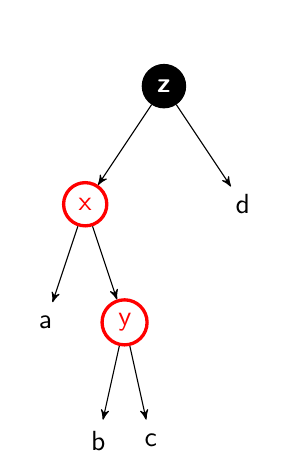
\begin{tikzpicture}[->,>=stealth',level/.style={sibling distance = 2.0cm/#1,
	level distance = 1.5cm}] 
\node [arn_n] {z}
child{ node [arn_r] {x} 
	child{ node [arn_x] {a} }
	child{ node [arn_r] {y}
		child{ node [arn_x] {b}}
		child{ node [arn_x] {c}}
	}                            
}
child{ node [arn_x] {d}
}
; 
\end{tikzpicture}
&& \\
&& $\Downarrow$ && \\
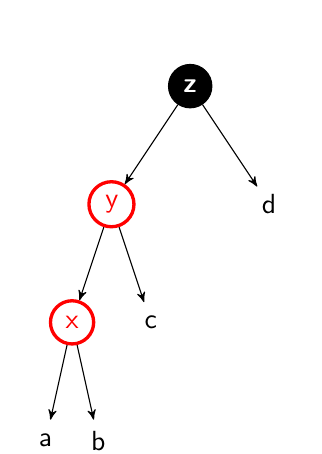
\begin{tikzpicture}[->,>=stealth',level/.style={sibling distance = 2.0cm/#1,
	level distance = 1.5cm}] 
\node [arn_n] {z}
child{ node [arn_r] {y} 
	child{ node [arn_r] {x}
		child{ node [arn_x] {a}}
		child{ node [arn_x] {b}}
	} 
	child{ node [arn_x] {c} }                           
}
child{ node [arn_x] {d}
}
; 
\end{tikzpicture} & $\Rightarrow$ & 
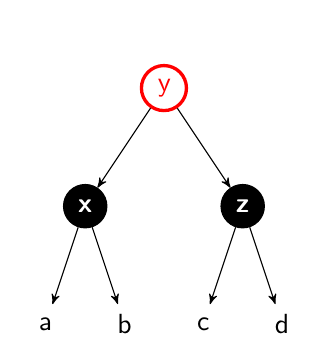
\begin{tikzpicture}[->,>=stealth',level/.style={sibling distance = 2.0cm/#1,
	level distance = 1.5cm}] 
\node [arn_r] {y}
child{ node [arn_n] {x} 
	child{ node [arn_x] {a} }
	child{ node [arn_x] {b} }                           
}
child{ node [arn_n] {z}
	child{ node [arn_x] {c}}
	child{ node [arn_x] {d}}
} 
; 
\end{tikzpicture} & 
$\Leftarrow$ &
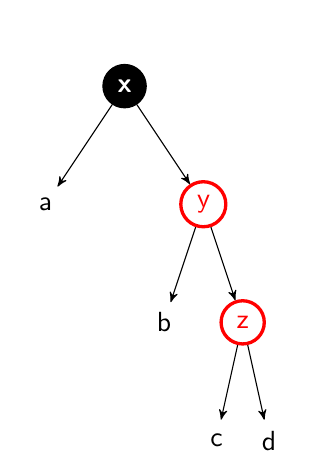
\begin{tikzpicture}[->,>=stealth',level/.style={sibling distance = 2.0cm/#1,
	level distance = 1.5cm}] 
\node [arn_n] {x}
child{ node [arn_x] {a}}
child{ node [arn_r] {y} 
	child{ node [arn_x] {b} }
	child{ node [arn_r] {z}
		child{ node [arn_x] {c}}
		child{ node [arn_x] {d}}
	}                            
}
; 
\end{tikzpicture} \\
&& $\Uparrow$ && \\[2cm]
&& 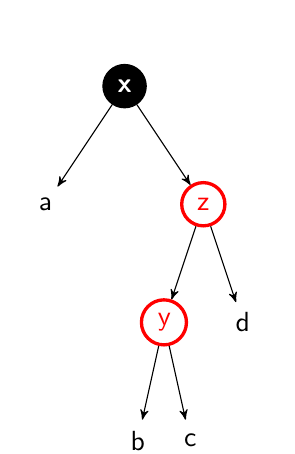
\begin{tikzpicture}[->,>=stealth',level/.style={sibling distance = 2.0cm/#1,
	level distance = 1.5cm}] 
\node [arn_n] {x}
child{ node [arn_x] {a}}
child{ node [arn_r] {z} 
	child{ node [arn_r] {y}
		child{ node [arn_x] {b}}
		child{ node [arn_x] {c}}
	} 
	child{ node [arn_x] {d} }                           
}
; 
\end{tikzpicture} &&
\end{tabular}
\end{center}
\end{fancyfig}

\task[task:adt-balance]{Complete the definition of the \haskellIn{balance} function, which given some arbitrary red-black tree, should balance it according to the transformations shown in \Cref{fig:rbtree-balance}. }

\clearpage 

You can accomplish this simply by pattern-matching on the tree given as input to determine whether it is unbalanced and returning a balanced version of it if necessary. One of the four transformations is already implemented for you.

\taskLine

\task[task:adt-insert]{Complete the definition of the \haskellIn{insert} function, which should insert some value of type \texttt{\small a} into a red-black tree. New nodes in the tree should initially be red. Use the \haskellIn{balance} function in the appropriate places to ensure that the resulting tree is balanced. The root of a red-black tree should always be black. For example, if you insert a bunch of elements from a list into a tree, the result in the REPL might look something like this:
}

\begin{minted}{haskell}
Lab4> foldl insert empty []
Leaf

Lab4> foldl insert empty [42]
Node Black Leaf 42 Leaf

Lab4> foldl insert empty ["CS141", "CS263"]
Node Black Leaf "CS141" (Node Red Leaf "CS263" Leaf)

Lab4> foldl insert empty "KOAN"
Node Black 
    (Node Black (Node Red Leaf 'A' Leaf) 'K' Leaf) 
    'N' 
    (Node Black Leaf 'O' Leaf)

Lab4> foldl insert empty "WITTER"
Node Black 
    (Node Black (Node Red Leaf 'E' Leaf) 
    'I' 
    (Node Red Leaf 'R' Leaf)) 'T' (Node Black Leaf 'W' Leaf)
\end{minted}

The exact result depends on the names you chose for your constructors and the order of their parameters. There are two unit tests for this lab which check that the depth of your red-black trees never exceed $2 \times \left \lfloor{\log(n+1)}\right \rfloor$ where $n$ is the number of nodes in the tree and that converting a red-black tree to a list results in a sorted list.

\task[task:adt-invariants]{There are two invariants which red-black trees should never violate:
\begin{enumerate}
	\item No red node has a red child.
	\item Every path from the root to a leaf contains the same number of black nodes.
\end{enumerate}
Convince yourself that these invariants are not violated by your implementation.
}

\taskLine

%\input{lectures/lecture9.tex}
%\input{lectures/lecture10.tex}
\section{Lazy evaluation}
\topics{Lazy evaluation, infinite data structures.}

These exercises are about lazy evaluation and infinite data structures. You can obtain the skeleton code by cloning the respective repository from GitHub:
\begin{minted}{bash}
$ git clone https://github.com/fpclass/lab-lazy-evaluation
\end{minted}

\makebox[0.5cm]{\faBook}~\emph{Recommended reading}: Chapter 15 of \emph{Programming in Haskell} \citep{hutton2016programming}.

\makebox[0.5cm]{\faBook}~\emph{Further reading}: if you want to read the full, gory technical details on how lazy evaluation is implemented by Haskell's runtime system, \emph{Implementing lazy functional languages on stock hardware: the Spineless Tagless G-machine} \citep{jones1992implementing} is for you.

\subsubsection{Infinite data structures}

In the lecture on lazy evaluation, you saw that Haskell supports infinite data structures such as infinite lists. This is possible because, at runtime, variables in Haskell are just pointers to closures. For example, we saw the following definition in the lecture:
\begin{minted}{haskell}
from :: Int -> [Int]
from n = n : from (n+1)
\end{minted}
Recall that the Haskell compiler transforms expressions which appear as arguments to functions into let-bound definitions:
\begin{minted}{haskell}
from :: Int -> [Int]
from n = let ns = from (n+1) in n : ns
\end{minted}
Thus, when \texttt{\small from n} is called for some \texttt{\small n}, a new closure for \texttt{\small ns} is allocated on the heap. Because of lazy evaluation, the call to \haskellIn{from (n+1)} is not evaluated immediately. It is only evaluated when the tail of \texttt{\small n~na:~ns} is needed and then the closure represented by \texttt{\small ns} is updated with the result of \haskellIn{from (n+1)}. The call to \haskellIn{from (n+1)} will allocate yet another closure for \haskellIn{from (n+2)} which is only evaluated when the tail of the tail of \haskellIn{from n} is needed.

\taskLine 

\task[task:ones]{Complete the definition of \haskellIn{ones} which should represent an infinite list where all elements are \haskellIn{1}.}

\taskLine

\pgfplotsset{width=7cm,compat=1.15}
\begin{fancyfig}{Time complexities of \haskellIn{foos} and \haskellIn{foos'}}{fig:foos-complexity}
	\begin{center}	
		\begin{tikzpicture} \begin{axis}
		[
		legend style={at={(1.5,1)},
			anchor=north,legend columns=-1},
		enlargelimits=0.15,
		ylabel=Time ($\mu$s),
		xlabel=Elements
		]
		\addplot+ [
		sharp plot,
		] coordinates {(10,0.994) (20,4.48)
			(30,10.2)};
		\addplot+ [
		sharp plot,
		] coordinates {(10,0.300) (20,0.610) 
			(30,0.919)};
		\legend{\texttt{foos},\texttt{foos'}}
		\end{axis}
		\end{tikzpicture}
	\end{center}
\end{fancyfig}

You also saw that the following definition for the infinite list of Fibonacci numbers can be implemented elegantly and efficiently as the following in Haskell:
\begin{minted}{haskell}
fibs :: [Integer]
fibs = 1 : 1 : zipWith (+) fibs (tail fibs)
\end{minted}
The infinite list represented by \haskellIn{fibs} can be generated in linear time for the number of elements requested. This is possible because \haskellIn{fibs} is transformed into the following:
\begin{minted}{haskell}
fibs :: [Integer]
fibs = let xs = tail fibs 
           ys = zipWith (+) fibs xs
           zs = 1 : ys
       in 1 : zs
\end{minted}
All closures involved in this definition can be updated with their results. Therefore, \haskellIn{fibs} refers to a cons cell (a kind of closure) where the head is \haskellIn{1} and the closure pointed to by \texttt{\small zs} is the tail. The closure represented by \texttt{\small zs} is also a cons cell where the head is \haskellIn{1} and the tail is pointed to by \texttt{\small ys}. The closure represented by \texttt{\small ys} will be updated with the result of \haskellIn{zipWith (+) fibs xs} when more than two elements are requested from \haskellIn{fibs}, \emph{i.e.} the tail of \texttt{\small zs} is inspected by a \haskellIn{case}-expression somewhere. The \haskellIn{zipWith} function, in turn, allocates more closures when called, thus recursively adding more cons cells as needed.

However, not all closures can be updated. Suppose we want to generalise the definition of \haskellIn{fibs} to sequences with arbitrary seed values \texttt{\small x} and \texttt{\small y}:
\begin{minted}{haskell}
foos :: Integer -> Integer -> [Integer]
foos x y = x : y : zipWith (+) (foos x y) (tail (foos x y))
\end{minted}
This will be exponentially slow, because Haskell will not update the closure for \haskellIn{foos} with the list that is being generated. As a result, every call to \haskellIn{foos x y} will result in the list being generated from the beginning. This makes sense, because \haskellIn{foos} is parametrised over \texttt{\small x} and \texttt{\small y} and it would be wrong to update the closure for \haskellIn{foos} with the list generated for some specific \texttt{\small x} and \texttt{\small y}. 

\taskLine

\task[task:arbitrary-sequence]{Implement \haskellIn{foos'} to produce the same sequence as \haskellIn{foos}, but in linear time. \emph{Hint}: you need to find a way to allocate a closure which is specific to some \texttt{\small x} and \texttt{\small y} and can be updated.}

\task[task:lazy-bench]{You can run \bashIn{stack bench} to compare the time complexities of \haskellIn{foos} and \haskellIn{foos'}. If you have done everything right, you should see a bar graph with similar growth as the graph shown in \Cref{fig:foos-complexity} in the \texttt{\small benchmark.html} file which is generated by \bashIn{stack bench}.}

\taskLine \newpage
\section{Equational reasoning}
\topics{Equational reasoning, constructive induction.}

Haskell is a purely functional programming language, which allows us to easily prove formal properties about our functions. This is nice because it means we do not have to rely on testing (which is not exhaustive) and can instead use structural induction to exhaustively cover all possible inputs to a function. The approach to proving properties we use for Haskell programs is called \emph{equational reasoning} -- this approach works by starting with an equation and rewriting both sides of it until they are the same. 

\makebox[0.5cm]{\faBook}~\emph{Recommended reading}: Chapters 16 and 17 of \emph{Programming in Haskell} \citep{hutton2016programming}.

\makebox[0.5cm]{\faLightbulbO}~If you are looking for more exercises, have a look at the past exam papers -- Question 4 on each paper has more theorems to prove.

\subsubsection{Induction on natural numbers}

Recall that we have already proved the following (monoidal) properties about natural numbers in the lecture on equational reasoning (\Cref{sec:lecture-10}):
\begin{displaymath}
\begin{array}{lcrcl}
\textbf{Left unit} &\qquad & \mathit{add}~Z~x & = & x \\
\textbf{Right unit} &\qquad & \mathit{add}~x~Z & = & x \\
\textbf{Associativity} & \qquad & \mathit{add}~x~(\mathit{add}~y~z) & = & \mathit{add}~(\mathit{add}~x~y)~z 
\end{array}
\end{displaymath}

Also recall the definition of \haskellIn{add} from \Cref{sec:lecture-10}:
\begin{displaymath}
\begin{array}{lllcl}
\multicolumn{5}{l}{\mathit{add} :: \mathit{Nat} \to \mathit{Nat} \to \mathit{Nat}} \\
\mathit{add} & Z & m & = & m \\
\mathit{add} & (S~n) & m & = & S~(\mathit{add}~n~m)
\end{array}
\end{displaymath}

\taskLine

\task[task:succ-comm]{Prove the following property about addition just by rewriting one side of the equation until you end up with the other side:
	\begin{displaymath}
	\forall n :: \mathit{Nat} . S~n = \mathit{add}~(S~Z)~n
	\end{displaymath}
	You should show each step of the proof along with a comment to say what you have done at that particular step, as shown in the lecture and the proofs in \Cref{sec:lecture-10}.
}

\task[task:successor-commutes]{Prove the following property about addition by induction on $n$. For this proof, you will need to make use of some of the other properties you know about $\mathit{add}$, including the one you proved for Exercise \ref{task:succ-comm}.
	\begin{displaymath}
	\forall n~m :: \mathit{Nat} . \mathit{add}~(S~n)~m = \mathit{add}~n~(S~m)
	\end{displaymath}
}

\task[task:add-commutes]{Finally, using all the properties you know about $\mathit{add}$ so far, prove that $\mathit{add}$ commutes:
	\begin{displaymath}
	\forall n~m :: \mathit{Nat} . \mathit{add}~n~m = \mathit{add}~m~n
	\end{displaymath}
}

\taskLine

\subsubsection{Induction on lists}

In Haskell, the \haskellIn{reverse} function can be defined as follows:
\begin{minted}{haskell}
reverse :: [a] -> [a]
reverse []     = []
reverse (x:xs) = reverse xs ++ [x]
\end{minted}
This makes use of the \haskellIn{(++)} operator, which is defined as follows:
\begin{minted}{haskell}
(++) :: [a] -> [a] -> [a]
[]     ++ ys = ys 
(x:xs) ++ ys = x : (xs ++ ys)
\end{minted}

\taskLine

\task[task:reverse-identity-left]{Prove that $(\append)$ has a left identity by rewriting the following equation:
	\begin{displaymath}
	\forall \mathit{xs} :: \hslist{a}~. \quad \hslist{} \append \mathit{xs} = \mathit{xs}
	\end{displaymath}}

\task[task:reverse-identity-right]{Prove that $(\append)$ has a right identity by induction on $\mathit{xs}$:
	\begin{displaymath}
	\forall \mathit{xs} :: \hslist{a}~. \quad \mathit{xs} \append \hslist{} = \mathit{xs}
	\end{displaymath}}

\task[task:append-assoc]{Prove that $(\append)$ is associative by induction on $\mathit{xs}$:
	\begin{displaymath}
	\forall \mathit{xs}~\mathit{ys}~\mathit{zs} :: \hslist{a}~. \quad \mathit{xs} \append (\mathit{ys} \append \mathit{zs}) = (\mathit{xs} \append \mathit{ys}) \append \mathit{zs}
	\end{displaymath}}

\task[task:reverse-preserves]{Prove that $\mathit{reverse}$ preserves singleton lists by rewriting the following equation:
	\begin{displaymath}
	\forall \mathit{x} :: a~. \quad \mathit{reverse}~\hslist{x} = \hslist{x}
	\end{displaymath}}

\task[task:reverse-distributes-over-append]{Prove that $\mathit{reverse}$ distributes over $(\append)$ by induction on $\mathit{xs}$. You will need some of the properties you have proved so far about $(\append)$ and $\mathit{reverse}$.
	\begin{displaymath}
	\forall \mathit{xs}~\mathit{ys} :: \hslist{a}~. \quad \mathit{reverse}~(\mathit{xs} \append \mathit{ys}) = \mathit{reverse}~\mathit{ys} \append \mathit{reverse}~\mathit{xs}
	\end{displaymath}}

\task[task:reverse-of-reverse]{Prove the following property about $\mathit{reverse}$ by induction on $\mathit{xs}$. You will need some of the properties you have proved so far about $(\append)$ and $\mathit{reverse}$.
	\begin{displaymath}
	\forall \mathit{xs} :: \hslist{a}~. \quad \mathit{reverse}~(\mathit{reverse}~\mathit{xs}) = \mathit{xs}
	\end{displaymath}}

\taskLine

\subsubsection{Constructive induction}

It is possible to use induction to \emph{calculate} faster function definitions. This is referred to as \emph{constructive induction}. For example, consider our current definition of \haskellIn{reverse}:
\begin{minted}{haskell}
reverse :: [a] -> [a]
reverse []     = []
reverse (x:xs) = reverse xs ++ [x]
\end{minted}
This definition is inefficient because the \haskellIn{(++)} operator runs in $\mathcal{O}(n)$ time where $n$ is the length of the first argument. The \haskellIn{reverse} function runs in quadratic time as a result. We can do better by combining the behaviour of \haskellIn{reverse} and \haskellIn{(++)} into one new function which does both. We begin by expressing this idea as the following specification:
\begin{minted}{haskell}
rev :: [a] -> [a] -> [a]
rev xs ys = reverse xs ++ ys
\end{minted}
The \haskellIn{rev} function takes two lists as arguments, reverses the first and then appends the second list to it. Our goal is now to use induction to come up with a new definition for \haskellIn{rev} which neither uses \haskellIn{reverse} nor \haskellIn{(++)}. We do this by taking the current definition and performing induction on \texttt{\small xs}. Recall that there are two cases for induction on lists: the empty list (a base case) and cons (a recursive case). We can write down a skeleton for the new definition of \haskellIn{rev} by covering these two cases:
\begin{minted}{haskell}
rev :: [a] -> [a] -> [a]
rev []     ys = ???
rev (x:xs) ys = ???
\end{minted} 

\task[task:rev-empty]{Replace the \texttt{\small ???} in the first equation by reducing \haskellIn{reverse [] ++ ys} as much as possible. The resulting expression should neither contain \haskellIn{reverse} nor \haskellIn{(++)}. \emph{Hint}: you only need to apply \haskellIn{reverse} and \haskellIn{(++)} until you are left with an expression which cannot be reduced any further. This expression can then be used as the right-hand side of the first equation above.}

\task[task:rev-cons]{Replace the \texttt{\small ???} in the second equation by reducing \haskellIn{reverse (x:xs) ++ ys} as much as possible. The resulting expression should neither contain \haskellIn{reverse} nor \haskellIn{(++)}. \emph{Hint}: in this case, you can use the specification \texttt{\small rev xs ys = reverse xs ++ ys} as induction hypothesis.}

\taskLine
 \newpage
\section{Foldables}
\topics{Foldables.}

These exercises are about foldables, \emph{i.e.} data structures for which we can implement \haskellIn{foldr}. As usual, you can obtain the skeleton code for this this lab by cloning the respective repository from GitHub:
\begin{minted}{bash}
$ git clone https://github.com/fpclass/lab-foldable
\end{minted}

\makebox[0.5cm]{\faBook}~\emph{Recommended reading}: Chapter 14 of \emph{Programming in Haskell} \citep{hutton2016programming}.

\taskLine 

\task{Consider the following definition of a data type for a simple expression language consisting of variables, integer values, and addition:}
\begin{minted}{haskell}
data Expr a = Var a
            | Val Int
            | Add (Expr a) (Expr a)
\end{minted}
This type is parametrised over some type \texttt{\small a} so that variables (the \haskellIn{Var} constructor) can be represented in different ways depending on what information needs to be associated with variables. This is useful if, for example, you are writing a compiler and want to initially only have variable names associated with your variables, but later add information such as types or line numbers. Some valid examples of \texttt{\small Expr} values are:
\begin{minted}{haskell}
e1 = Var "x"
e2 = Var ("x",22)
e3 = Val 4 
e4 = Add (Val 8) (Var "y")
e5 = Add (Val 8) (Var 7)
e6 = Add e2 (Var ("y",42))
e7 = Add e6 e6
\end{minted}
Complete the \haskellIn{Foldable} instance for \texttt{\small Expr}. Once implemented, you should be able to do the following in the REPL:
\begin{minted}{haskell}
toList e3 ==> []
toList e5 ==> [7]
sum e5    ==> 7
toList e7 ==> [("x",22),("y",42),("x",22),("y",42)]
length e7 ==> 4
\end{minted}

\taskLine

\task{A useful data structure in purely functional programming languages is the \emph{zipper}. Zippers can help make traversing data structures more efficient if repeated access to one element is required. Zippers can be defined for arbitrary data structures, but to keep things simple we will only look at lists. For lists, the zipper is defined as shown in the code snippet below:}
\begin{minted}{haskell}
data Zipper a = Zipper [a] a [a]
\end{minted}
The zipper for lists is a bit like a Turing tape: we have an element of type \texttt{\small a} that is in the ``view'' and we have elements to the ``left'' of it (the first \texttt{\small [a]}) as well as to the ``right'' of it (the second \texttt{\small [a]}). We can convert ordinary, non-empty lists into zippers with a function of type:
\begin{minted}{haskell}
fromList :: [a] -> Zipper a
\end{minted}
This should work as follows: the head of the input list should be the element that is in the ``view'' and the tail of the input list should be to the ``right'' of the element in the ``view''. Implement this function now and ensure that the tests for it pass.

\task{There are three useful functions to work with zippers. Their type signatures are:}
\begin{minted}{haskell}
view  :: Zipper a -> a 
left  :: Zipper a -> Zipper a 
right :: Zipper a -> Zipper a
\end{minted}
The \haskellIn{view} function simply retrieves the element that is in the ``view''. If the list of elements to the ``right`` of the ``view`` is not empty, the \haskellIn{left} function shifts elements to the ``left'' so that the ``view'' of the input is the first element on the ``left'' and that the first element of the ``right'' of the input is then in the ``view''. The \haskellIn{right} function does the opposite and shifts elements to the ``right''. Implement all three functions now and ensure that the tests pass.

\task{The \texttt{\small Zipper} type can be made an instance of \haskellIn{Foldable}. Complete the definition of \haskellIn{foldr} for it now. In essence, this should satisfy the following equations:}
\begin{minted}{haskell}
toList (fromList xs) == xs
foldr f z (fromList xs) == foldr f z xs
\end{minted}

\taskLine 

\task{As we have seen in the lectures, we can define very useful functions that work for any type provided that a \haskellIn{Foldable} instance exists. Generalise the \haskellIn{filter} function to a function \haskellIn{filterF} which should work on all types that have an instance of \haskellIn{Foldable}. Some examples of its usage are shown below:}
\begin{minted}{haskell}
filterF ((=="x") . fst) e7               ==> [("x",22),("x",22)]
filterF (>5) (Zipper [1,5,10] 8 [6,7,2]) ==> [10,8,6,7]
\end{minted}

\task{Could you define an even more general \haskellIn{filter} function which can return the filtered elements in an arbitrary data structure that satisfies some type class constraints? In other words, a function with \emph{e.g.} the following typing where \haskellIn{???} should be replaced by your type class constraints:}
\begin{minted}{haskell}
filterFA :: (Foldable f, ??? g) => (a -> Bool) -> f a -> g a
\end{minted}

\taskLine 

\task{We can write \emph{even more} generic, useful functions by combining multiple type class constraints. For example: }
\begin{minted}{haskell}
asum :: (Alternative f, Foldable t) => t (f a) -> f a
\end{minted}
Implement this function in terms of \haskellIn{foldr} and \haskellIn{(<|>)} so that combines the elements of some data structure with \haskellIn{(<|>)}. See below for examples of \haskellIn{asum} in action:
\begin{minted}{haskell}
asum [Nothing, Just 4, Nothing]                   ==> Just 4
asum (Zipper [Just 4, Nothing] (Just 5) [])       ==> Just 4
asum (Zipper [Nothing, Nothing] (Just 5) [])      ==> Just 5
asum (Zipper [Nothing, Nothing] Nothing [Just 1]) ==> Just 1
\end{minted}

\taskLine  \newpage
\section{Functors}
\topics{Functors.}

These exercises are about functors. We introduce you to a range of different types that are functors, in addition to those that you have seen in the lectures. Many of the types you will work with in these exercises may seem outright silly at this point. However, they we will continue to work with them in the coming weeks and you will see how they become increasingly more useful as we get to know more and more abstractions. As usual, you can obtain the skeleton code by cloning the respective repository from GitHub with the following command:
\begin{minted}{bash}
$ git clone https://github.com/fpclass/lab-functors
\end{minted}

\taskLine

\task{We start off with one of the simplest types that is a functor: the \texttt{\small Identity} type. This type is defined as follows:}
\begin{minted}{haskell}
data Identity a = Identity a
\end{minted}
This may seem like quite a silly type to define -- what is it good for? We will find out later. For now, define an instance of \haskellIn{Functor} for it. Once defined, using \haskellIn{fmap} will have the same effect as just applying a function directly to the value that we put inside of \haskellIn{Identity}:
\begin{minted}{haskell}
fmap (+2) (Identity 4)              ==> Identity 6
fmap length (Identity "Witter")     ==> Identity 6
fmap ($ "cake") (Identity length)   ==> Identity 4
fmap (map (=='o')) (Identity "foo") 
==> Identity [False,True,True]
\end{minted} 

\task[task:identity-functor]{Once you have implemented \haskellIn{fmap}, you may wish to verify that your instance of \haskellIn{Functor} for \texttt{\small Identity} obeys the functor laws. Running the tests with \bashIn{stack test} will give you some indication, but you could also do it formally with some proofs by induction for the two functor laws.}

\taskLine 

\task{Another type that looks just as silly is the \texttt{\small Const} type which can be defined as:}
\begin{minted}{haskell}
data Const v a = Const v
\end{minted}
This type is also a functor. Complete the \haskellIn{Functor} instance for it. Once implemented, you can test it's behaviour (or rather lack thereof):
\begin{minted}{haskell}
fmap (+2) (Const 4)              ==> Const 4
fmap length (Const "Witter")     ==> Const "Witter"
fmap (map (=='o')) (Const "foo") ==> Const "foo"
\end{minted} 
As we can see, the ``effect'' of this functor is that it always preserves the values stored inside of it and the function we apply with \haskellIn{fmap} does nothing. 

\task[task:const-functor]{You may again wish to convince yourself that your implementation of \haskellIn{fmap} for this type obeys the functor laws.}

\taskLine 

\task{You are given a definition for a type \texttt{\small Point} that can be used to represent points in two-dimensional space as well as other pairs of values of the same type:   }
\begin{minted}{haskell}
data Point a = Point a a
\end{minted}
For example, some values of this type are:
\begin{minted}{haskell}
p1 :: Point Int
p1 = Point 4 5

p2 :: Point Double
p2 = Point 2.3 4.2 

p3 :: Point String
p3 = Point "hello" "world" 
\end{minted}
The \texttt{\small Point} type is a functor. Complete the \haskellIn{Functor} instance for it. Some examples of what you should be able to do with the \haskellIn{Functor} instance for \texttt{\small Point} are:
\begin{minted}{haskell}
fmap (+1) p1   ==> Point 5 6 
fmap (+1) p2   ==> Point 3.3 5.2 
fmap show p2   ==> Point "2.3" "4.2"
fmap length p3 ==> Point 5 5
\end{minted}
As you can see, having \haskellIn{fmap} available for a type allows us to perform quite the range of operations on values of the \texttt{\small Point} type.

\task[task:point-functor]{You may once again wish to verify that your instance of \haskellIn{Functor} for \texttt{\small Point} obeys the functor laws.}

\taskLine \pagebreak

\task{Consider the following definition of \emph{rose trees}:}
\begin{minted}{haskell}
data RoseTree a = Leaf a | Node [RoseTree a]
\end{minted}
In a rose tree, every node can have zero or more children. This type is also a functor. Complete the instance of \haskellIn{Functor} for \texttt{\small RoseTree}. Below are some examples of what is possible with \haskellIn{fmap} for \texttt{\small RoseTree}:

\begin{minted}{haskell}
fmap (+5) (Leaf 4)                ==> Leaf 9 
fmap (+5) (Node [])               ==> Node []
fmap (+5) (Node [Leaf 4, Leaf 8]) ==> Node [Leaf 9, Leaf 13]
fmap length (Node [Node [], Node [Leaf "duck"]])
==> Node [Node [], Node [Leaf 4]]
fmap sum (Node [Node [Leaf [1,2,3]], Node [Leaf [9,8,7]]])
==> Node [Node [Leaf 6], Node [Leaf 24]]
\end{minted}

\taskLine 

\task{A property of functors is that, given any two functors, they can be composed to form a new functor which combines both. This is useful if, for example, we want to exploit the fact that lists are functors to work more easily with nested lists. To begin, let us define a suitable type to represent a data structure where values of type \texttt{\small g a} are nested inside containers of type \texttt{\small f}:}
\begin{minted}{haskell}
data Compose f g a = Compose (f (g a))
\end{minted}
This type is a functor. Complete the respective instance of \haskellIn{Functor}. Once implemented, you can very easily apply \haskellIn{fmap} to arbitrarily nested data structures: 
\begin{minted}{haskell}
fmap (+5) (Compose [[1,2,3], [4,5,6]]) 
==> Compose [[6,7,8], [9,10,11]]
fmap not (Compose [Just True, Just False, Nothing])
==> Compose [Just False, Just True, Nothing]
fmap even (Compose (Node [Leaf [1,2,3]]))
==> Compose (Node [Leaf [False, True, False]])
fmap (+5) (Compose (Compose [[[1,2],[3]], [[4],[5,6]]]))
==> Compose (Compose [[[6,7],[8]],[[9],[10,11]]])
\end{minted}

\task[task:compose-functor]{Proving that \haskellIn{fmap} for \texttt{\small Compose} obeys the functor laws is significantly more interesting than for the previous types. Can you do it? \emph{Hint}: you need to assume that the two underlying functors obey the laws and make use of them.}

\taskLine \pagebreak

Consider the following definition of a data type in Haskell:
\begin{minted}{haskell}
data State s a = St (s -> (a,s))
\end{minted}
This type, which we have named \texttt{\small State}, has two type parameters \texttt{\small s} and \texttt{\small a}. It has a single data constructor, named \haskellIn{St}, which has a single parameter of type \texttt{\small s -> (a,s)}. Therefore, the type of \haskellIn{St} is \texttt{\small (s -> (a,s)) -> State s a}. In other words, given a function of type \texttt{\small s -> (a,s)}, the \haskellIn{St} constructor produces a value of type \texttt{\small State s a}. Our intuition for this type is going to be that \haskellIn{St} is a wrapper around ``stateful'' functions: that is, functions which require some initial state (of some type \texttt{\small s}) as argument and return a pair consisting of a result (of some type \texttt{\small a}) and a potentially new state (of the same type \texttt{\small s} as the initial state). For example, we could define the following value of \texttt{\small State Int Int}:
\begin{minted}{haskell}
fresh :: State Int Int 
fresh = St (\s -> (s, s+1))
\end{minted}
Let us also define a little helper function that is useful to have when working with the \texttt{\small State} type, which extracts the function \texttt{\small m} of type \texttt{\small s -> (a,s)} from a value of type \texttt{\small State s a} and applies it to some initial state \texttt{\small s} of type \texttt{\small s}:
\begin{minted}{haskell}
runState :: State s a -> s -> (a, s)
runState (St m) s = m s
\end{minted}
Using both of these definitions, we can then get some results:
\begin{minted}{haskell}
runState fresh 4                                   ==> (4,5)
runState fresh 7                                   ==> (7,8)
let (x,s') = runState fresh 7 in runState fresh s' ==> (8,9)
\end{minted}
While this is currently not overly interesting and a rather clunky, these definitions will provide the foundations for much more exciting things that are yet to come...

\task{Meanwhile, back to the grind: the \texttt{\small State} type is a functor. Complete the definition of \haskellIn{fmap} for it. Some examples of it in action:}
\begin{minted}{haskell}
runState (fmap (*2) fresh) 4 ==> (8,5) 
runState (fmap show fresh) 7 ==> ("7",8)
\end{minted}
\emph{Hint}: implementing \haskellIn{fmap} for \texttt{\small State} is mostly a game with types. If you are unsure of what to write, place a typed hole \haskellIn{_} in the place where you do not know what expression to use and the Haskell compiler will tell you what the type of the expression should be, what variables are in scope and what their types are.

\taskLine 

\task{We know that, in Haskell, functions have types of the form \texttt{\small a -> b} where \texttt{\small a} is the domain of the function (\emph{i.e.} the type of arguments that the function accepts) and \texttt{\small b} is the co-domain (\emph{i.e.} the type of values the function produces). In Haskell, type constructors can be partially applied just like functions. For example, \texttt{\small (->) a}, is the function type constructor \texttt{\small (->)} applied to only one argument \texttt{\small a}. Of course there are no values of this type, so why is this useful? Well, it turns out that this type is a functor! Can you complete the definition of \haskellIn{Functor} for it and figure out what \haskellIn{fmap} does for this type? }
\begin{minted}{haskell}
instance Functor ((->) r) where 
    -- fmap :: (a -> b) -> (r -> a) -> (r -> b)
    fmap = undefined
\end{minted}
\emph{Hint}: this is very easy if you recognise the type of \haskellIn{fmap} where \texttt{\small f} is replaced by \texttt{\small(->) r} (shown in the comment above) from somewhere... \newpage
\section{Applicative functors}
\topics{Applicative functors, parsing.}

These exercises are about using applicative functors. As usual, you can obtain the skeleton code for this this lab by cloning the respective repository from GitHub:
\begin{minted}{bash}
$ git clone https://github.com/fpclass/lab-applicatives
\end{minted}
The aim of this lab is to implement a small library for constructing \emph{parsers} as well as to build a parser for a small expression language. At the end of this lab, we will have a function called \haskellIn{parseAndEval} which, given a string representation of simple arithmetic expressions, will be able to convert them into a value of an \haskellIn{Expr} type which is then interpreted. The \haskellIn{parseAndEval} function may fail if the input string is not well formatted. Here are a few examples of how it will work:
\begin{minted}{haskell}
parseAndEval "4"                   ==> Just 4
parseAndEval "(15 + 16)"           ==> Just 31
parseAndEval "((2 + 4) + (9 + 2))" ==> Just 17
parseAndEval "(2"                  ==> Nothing
\end{minted}

\subsubsection{Parsers}

A parser is a program which, given some text as input, attempts to convert it into a more structured representation in memory. For example, a parser might be part of a compiler where it converts code written in a particular programming language into a representation that the compiler can work with, such as a type like \texttt{\small Expr} that we have seen in the lectures. We can therefore think of parsers as functions of the following type:
\begin{center}
	\texttt{\small String -> Maybe (a, String)}
\end{center}
That is, given a value of type \texttt{\small String} as input, a parser consumes some of the input and tries to return a value of some type \texttt{\small a} (the structured representation) as well as all of the remaining input. However, it may fail and return \haskellIn{Nothing} if the input does not contain something in the format expected by a particular parser. One approach to constructing parsers is called \emph{parser combinators}. The idea is to have a library of very basic parsers, such as one which parses a single character or one which allows choice between two different parsers, and combine them to construct more meaningful parsers. With this in mind, we define a type of parser computations as an algebraic data type. This will ultimately allow us to make the input to individual parsers implicit:
\begin{minted}{haskell}
data Parser a = MkParser (String -> Maybe (a, String))
\end{minted}
A value of type \texttt{\small Parser a} represents a parser computation which returns a value of \texttt{\small a}. The \haskellIn{MkParser} data constructor has type \texttt{\small (String -> Maybe (a, String)) -> Parser a}. That is, given some function which implements the parsing behaviour, a value of type \texttt{\small Parser a} is returned. You are given a function
\begin{minted}{haskell}
parse :: Parser a -> String -> Maybe a
\end{minted}
which, given a computation of type \texttt{\small Parser a} and an input \texttt{\small String}, may return some value of type \texttt{\small a} wrapped into \haskellIn{Just} or \haskellIn{Nothing} if parsing failed.

\taskLine 

\task[task:parser-ch]{Implement the \haskellIn{ch} function which, given a predicate on \texttt{\small Char} values, should construct a parser which inspects the first character in its input: if the first character satisfies the predicate, then the character should be returned together with the remaining input. If the first character does not satisfy the predicate or the input is empty, then the parser should return \haskellIn{Nothing}:}
\begin{minted}{haskell}
parse (ch (=='x')) ""    ==> Nothing
parse (ch (=='x')) "yzx" ==> Nothing
parse (ch (=='x')) "xyz" ==> Just ('x',"yz")
\end{minted}

\taskLine 

\task[task:parser-functor]{The \texttt{\small Parser} type is a functor where we can apply functions of type \texttt{\small a -> b} to the result of the parser. Complete the \texttt{\small Functor} instance for \texttt{\small Parser} by replacing \haskellIn{undefined} with suitable code:}
\begin{minted}{haskell}
instance Functor Parser where 
    -- fmap :: (a -> b) -> Parser a -> Parser b
    fmap f (MkParser p) = undefined
\end{minted}
Once implemented, you should be able to run the following expressions in the REPL to get the results shown:
\begin{minted}{haskell}
parse (fmap isUpper (ch (=='x'))) "xyz"    ==> Just (False,"yz")
parse (fmap isUpper (ch (=='y'))) "xyz"    ==> Nothing
parse (fmap digitToInt (ch isDigit)) "1xy" ==> Just (1,"xy")
parse (fmap digitToInt (ch isDigit)) "xy"  ==> Nothing
\end{minted}

\taskLine 

\task[task:parser-pure]{The \texttt{\small Parser} type is also an applicative functor. The \haskellIn{pure} function should construct a parser which does not touch its input and always returns the argument of type \texttt{\small a} that is given to \haskellIn{pure}:}
\begin{minted}{haskell}
instance Applicative Parser where
   -- pure :: a -> Parser a
   pure x = undefined
\end{minted}
Once you have implemented \haskellIn{pure}, the following expressions should evaluate to the results shown:
\begin{minted}{haskell}
parse (pure True) "xyz" ==> Just (True, "xyz")
parse (pure True) ""    ==> Just (True, "")
parse (pure 42) "123"   ==> Just (42, "123")
\end{minted}

\task[task:parser-applicative]{The \haskellIn{(<*>)} operator should compose two parsers into one parser. For \texttt{\small Parser}, it has the following type:}
\begin{minted}{haskell}
(<*>) :: Parser (a -> b) -> Parser a -> Parser b
\end{minted}
That is, given two parsers where one returns a function of type \texttt{\small a -> b} and one returns a value of type \texttt{\small a}, it should construct a parser which combines the two parsers given as arguments into one parser that returns a value of type \texttt{\small b}. You are given the following skeleton:
\begin{minted}{haskell}
(MkParser a) <*> p = MkParser $ \xs -> case a xs of
    Nothing      -> undefined
    Just (f, ys) -> let (MkParser b) = p in case b ys of
        Nothing      -> undefined
        Just (x, zs) -> undefined
\end{minted}
The intuition here is that \haskellIn{(<*>)} returns a computation of type \texttt{\small Parser b}, \emph{i.e.} a parser computation which returns a value of type \texttt{\small b}. This computation is defined using the \haskellIn{MkParser} constructor applied to a parsing function, which takes a string \texttt{\small xs} as input, then applies the parsing function \texttt{\small a}, obtained from pattern-matching on the computation of type \texttt{\small Parser (a -> b)}, to it. This either results in failure, in which case the whole thing you should fail (you need to fill in this behaviour for the first \haskellIn{undefined}). If \texttt{\small a xs} is successful, then the result is a function \texttt{\small f~::~a -> b} and the remaining input \texttt{\small ys~::~String}. We then pattern-match on \texttt{\small p~::~Parser a} to obtain the second parsing function \texttt{\small b~::~String -> Maybe (a, String)} which we then apply to the remaining input \texttt{\small ys} obtained from evaluating the first parsing function. Applying \texttt{\small b} to \texttt{\small ys} results in a computation of type \texttt{\small Maybe (a, String)} so we pattern-match on it to determine whether it failed or succeeded. If it failed, the whole thing should fail again (you need to implement this behaviour where the second \haskellIn{undefined} is). If the second parsing function succeeds, then we get a result \texttt{\small x~::~a} and the remaining input \texttt{\small zs~::~String}. You now need to replace the third \haskellIn{undefined} with a value of type \texttt{\small Maybe (b, String)} which should indicate success and contain the result of applying \texttt{\small f} to \texttt{\small x} alongside the remaining input of the second parsing function. Once you have implemented \haskellIn{(<*>)}, the following expressions should evaluate to the results shown:
\begin{minted}{haskell}
parse (pure digitToInt <*> ch isDigit) "1yz" 
==> Just (1,"yz")
parse (pure digitToInt <*> ch isDigit) "xyz" 
==> Nothing 
parse ((\x y -> [x,y]) <$> ch isDigit <*> ch isDigit) "123" 
==> Just ("12","3")
parse ((\x y -> [x,y]) <$> ch isDigit <*> ch isDigit) "x23" 
==> Nothing
parse ((\x y -> [x,y]) <$> ch isDigit <*> ch isDigit) "1x3" 
==> Nothing
\end{minted}

\taskLine

\subsubsection{Alternatives}

When working with applicative functors, it is sometimes useful to express the notion of choice. For example, in the case of parsers, if one parser returns failure, we may want to try a different parser to see if it succeeds instead. The \haskellIn{Alternative} type class provides some functions and operators to support this idea:
\begin{minted}{haskell}
class Applicative f => Alternative f where
    empty :: f a
    (<|>) :: f a -> f a -> f a

    some  :: f a -> f [a]
    some p = (:) <$> p <*> many p

    many  :: f a -> f [a]
    many p = some p <|> pure []
\end{minted}

\taskLine

\task[task:parser-empty]{For the \texttt{\small Parser} type, the \haskellIn{empty} value has type \texttt{\small Parser a}. It should represent a computation which \emph{always} fails. For example:}
\begin{minted}{haskell}
parse empty "xyz"                                 ==> Nothing
parse (const <$> ch (const True) <*> empty) "xyz" ==> Nothing
\end{minted}
As an aside, \haskellIn{ch (const True)} is a parser which will accept any character.

\task[task:parser-or]{The \haskellIn{(<|>)} operator has type \texttt{\small Parser a -> Parser a -> Parser a} for the \haskellIn{Alternative} instance for \texttt{\small Parser}. The intuition with this operator is that it will try the first parser. If the first parser succeeds, then its result is returned. Otherwise, the second parser is used and its result determines the overall result. For example:}
\begin{minted}{haskell}
parse (ch (=='x') <|> ch (=='y')) "x12" ==> Just ('x', "12")
parse (ch (=='x') <|> ch (=='y')) "y12" ==> Just ('y', "12")
parse (ch (=='x') <|> ch (=='y')) "z12" ==> Nothing
parse (ch (=='x') <|> ch isDigit) "y12" ==> Nothing
parse (ch (=='x') <|> ch isDigit) "x12" ==> Just ('x', "12")
parse (ch (=='x') <|> ch isDigit) "012" ==> Just ('0', "12")
\end{minted}

\task[task:parser-alternatives]{The \haskellIn{some} and \haskellIn{many} functions may be used to repeatedly invoke \texttt{\small p} and to generate a list of the results. While \haskellIn{some} should only succeed with the list of results obtained from \texttt{\small p} if \texttt{\small p} succeeds at least once, \haskellIn{many} should also return with the list of results obtained from \texttt{\small p} but may return the empty list if \texttt{\small p} does not even succeed once. You will have to implement either \haskellIn{some} or \haskellIn{many} as the default implementations are defined in terms of each other. For example:}
\begin{minted}{haskell}
parse (some (ch isDigit)) "xyz"    ==> Nothing
parse (many (ch isDigit)) "xyz"    ==> Just ("", "xyz")
parse (some (ch isDigit)) "1xyz"   ==> Just ("1", "xyz")
parse (many (ch isDigit)) "1xyz"   ==> Just ("1", "xyz")
parse (some (ch isDigit)) "123xyz" ==> Just ("123", "xyz")
parse (many (ch isDigit)) "123xyz" ==> Just ("123", "xyz")
\end{minted}

\taskLine

\subsubsection{Parser combinators}

We can now define some basic parsers for common things we might wish to do. We will later be able to combine these basic parsers into more sophisticated parsers. 

\taskLine 

\task[task:parser-token]{Complete the definition of \haskellIn{token}, which should return the result of \texttt{\small p} which may be preceded by zero or more whitespace characters. The \texttt{\small whitespace :: Parser String} computation will be of use, which parses zero or more whitespace characters.}
\begin{minted}{haskell}
parse (token (ch (=='?'))) "?"     ==> Just ('?', "")
parse (token (ch (=='?'))) "    ?" ==> Just ('?', "")
\end{minted}
\emph{Hint}: The \haskellIn{(*>)} and \haskellIn{(<*)} from the lecture on applicative functors will be useful for this definition as well as coming ones.

\task[task:parser-between]{Complete the definition of \haskellIn{between}, which should return the result of \texttt{\small p}. \texttt{\small p} should be preceded by \texttt{\small open} and followed by \texttt{\small close}, the results of which should be discarded.}
\begin{minted}{haskell}
parse (between (ch (=='{')) (ch (=='}')) nat) "123}"  
==> Nothing
parse (between (ch (=='{')) (ch (=='}')) nat) "{123"  
==> Nothing
parse (between (ch (=='{')) (ch (=='}')) nat) "{123}" 
==> Just (123,"") 
\end{minted}

\taskLine 

\subsubsection{Expression language}

The final part of this exercise is to implement a parser for a small expression language using the parser combinators and type class instances we have implemented so far. Expressions in this language are represented by the following algebraic data type:
\begin{minted}{haskell}
data Expr = Val Int | Add Expr Expr
\end{minted}
Given a value of type \texttt{\small Expr}, we can map it to a corresponding \texttt{\small Int} value with the help of the following function (an interpreter):
\begin{minted}{haskell}
eval :: Expr -> Int 
eval (Val n)   = n
eval (Add l r) = eval l + eval r
\end{minted}

\taskLine 

\task[task:hutton-prims]{With the help of \haskellIn{token} and \haskellIn{ch}, implement the \haskellIn{lparen}, \haskellIn{rparen}, and \haskellIn{plus} parsers. The \haskellIn{lparen} parser should parse \texttt{\small (}, \haskellIn{rparen} should parse \texttt{\small )}, and \haskellIn{plus} should parse \texttt{\small +}. Each may optionally be preceded by whitespace which should be ignored: }
\begin{minted}{haskell}
parse lparen "("    ==> Just ('(', "")
parse lparen "   (" ==> Just ('(', "")
parse rparen ")"    ==> Just (')', "")
parse rparen "   )" ==> Just (')', "")
parse plus "+"      ==> Just ('+', "")
parse plus "   +"   ==> Just ('+', "")
\end{minted}

\task[task:hutton-expr-parser]{Implement the \haskellIn{expr} parser which should either accept \haskellIn{val} or \haskellIn{add}.}

You should now be able to run \haskellIn{parseAndEval} on strings containing simple arithmetic expressions as shown in the introduction to this lab.

\taskLine  \newpage
\section{Effectful Programming}
\topics{Monads.}

These exercises are about monads. As usual, you can obtain the skeleton code for the exercises by cloning the respective repository from GitHub:
\begin{minted}{bash}
$ git clone https://github.com/fpclass/lab-effectful-programming
\end{minted}
For your reference, the definition of the \haskellIn{Monad} type class is given below. A type \texttt{\small m} is a monad if it is an applicative functor and there is a function of type \texttt{\small m~a -> (a -> m~b) -> m~b} which satisfies the monad laws. This function is referred to as ``bind'' and denoted by the  \haskellIn{(>>=)} operator. In Haskell, we can overload the \haskellIn{(>>=)} operator for all types which are monads using a type class:
\begin{minted}{haskell}
class Applicative m => Monad m where 
    return :: a -> m a 
    return = pure 
    
    (>>=) :: m a -> (a -> m b) -> m b
\end{minted}
Also for your reference, the monad laws are shown below:
\begin{displaymath}
\begin{array}{lcrcl}
\textbf{Left identity} &\qquad & \mathit{return}~x \bind f & = & f~x \\
\textbf{Right identity} &\qquad & m \bind \mathit{return} & = & m \\
\textbf{Associativity} & \qquad & (m \bind f) \bind g & = & m \bind (\lambda x \to f~x \bind g)
\end{array}
\end{displaymath}

\faBook~\emph{Recommended reading}: Chapters 12 and 13 of \emph{Learn you a Haskell} \citep{lipovaca2011learn} or Chapter 12 of \emph{Programming in Haskell} \citep{hutton2016programming}.

\faBook~\emph{Further reading}: the use of monads in functional programming was popularised by \emph{Monads for functional programming} \citep{wadler1995monads}.

\taskLine 

\task[task:grandparent]{Suppose that you are given a family tree of the Duck family. The family tree is represented as a Haskell list of pairs which maps the names of members of the Duck family to their respective parent:}
\begin{minted}{haskell}
duckily :: [(String, String)]
duckily =
    [ ("Grandduck", "Grand duckster")
    , ("Baby Duck", "Parent Duck")
    , ("Duckling", "Older duckling")
    , ("Parent Duck", "Grandduck")
    ]
\end{minted}
Using the \haskellIn{lookup} function and the fact that \texttt{\small Maybe} is a monad, write a function 
\begin{minted}{haskell}
grandduck :: [(String, String)] -> String -> Maybe String
\end{minted}
which, given a family tree in the format shown above and the name of a member of the family, should retrieve its grandparent if there is one known:
\begin{minted}{haskell}
grandduck duckily "Baby Duck"   ==> Just "Grandduck"
grandduck duckily "Duckling"    ==> Nothing
grandduck duckily "Parent Duck" ==> Just "Grand duckster"
\end{minted}

\task[task:grandduck-applicative]{Could you define the \haskellIn{grandduck} function if \texttt{\small Maybe} was only an applicative functor? If not, why?}

\taskLine 

\task[task:mapM]{The \haskellIn{map} function can be generalised to a \haskellIn{mapM} function which allows the function given as argument to return a monadic computation and sequences those computations:}
\begin{minted}{haskell}
mapM :: Monad m => (a -> m b) -> [a] -> m [b]
mapM f []     = return [] 
mapM f (x:xs) = do 
    y  <- f x 
    ys <- mapM f xs
    return (y:ys)
\end{minted}
For example:
\begin{minted}{haskell}
mapM (safediv 4) [1,2,4] ==> Just [4,2,1]
mapM (safediv 4) [1,0,4] ==> Nothing
\end{minted}
This version of \haskellIn{mapM} is defined with the help of the \haskellIn{do}-notation, which is just syntactic sugar for \haskellIn{(>>=)} and anonymous functions. Show what the definition of \haskellIn{mapM} given above would look like without the \haskellIn{do}-notation, \emph{i.e.} what the compiler desugars it into.

\task[task:mapA]{Can you define the same function as \haskellIn{mapM}, but only with an \haskellIn{Applicative} constraint instead of \haskellIn{Monad}?}

\task[task:zipWithM]{The \haskellIn{zipWith} function we encountered previously can also be generalised to functions which return monadic computations:}
\begin{minted}{haskell}
zipWithM :: Monad m => (a -> b -> m c) -> [a] -> [b] -> m [c]
\end{minted}
Implement this function so that the following expressions result in the values shown:
\begin{minted}{haskell}
zipWithM safediv [] [1,2,3]    ==> Just []
zipWithM safediv [4,5,6] []    ==> Just []
zipWithM safediv [4,5] [1,2,0] ==> Just [4,2]
zipWithM safediv [4,5,6] [1,0] ==> Nothing
zipWithM (\x y -> [x,y]) [1,2] [3,4] 
==> [[1,2],[1,4],[3,2],[3,4]]
\end{minted}

%\task[task:zipWithA]{Could you implement a \texttt{zipWithA} function which behaves like \texttt{zipWithM} and has the same type, except that the \texttt{Monad} constraint has been replaced by an \texttt{Applicative} constraint?}

\taskLine

The \texttt{\small Either} type is similar to the \texttt{\small Maybe} type in that it can be used to indicate success and failure. Unlike the \texttt{\small Maybe} type, whose \haskellIn{Nothing} constructor takes no arguments, the \haskellIn{Left} constructor of \texttt{\small Either a b} takes one argument of type \texttt{\small a} which can be used to provide more information about the reason of the failure.

\task[task:either-functor]{The \texttt{\small Either} type is a functor. Complete the instance of \haskellIn{Functor} for it so that:}
\begin{minted}{haskell}
fmap (+5) (Left "Witter") ==> Left "Witter" 
fmap (+5) (Left Nothing)  ==> Left Nothing
fmap (+5) (Right 8)       ==> Right 13
\end{minted}

\task[task:either-applicative]{The \texttt{\small Either} type is an applicative functor. Complete the instance of \haskellIn{Functor} for it so that the following expressions evaluate to the values shown:}
\begin{minted}{haskell}
pure (+4) <*> Right 42      ==> Right 46 
pure (+4) <*> Left "Koan"   ==> Left "Koan"
(+) <$> Right 4 <*> Right 2 ==> Right 6
(+) <$> Left 4 <*> Right 2  ==> Left 4
(+) <$> Right 4 <*> Left 2  ==> Left 2
\end{minted}

\task[task:either-monad]{The \texttt{\small Either} type is a monad. Complete the instance of \haskellIn{Monad} for it so that the following expressions evaluate to the values shown:}
\begin{minted}{haskell}
Right 5 >>= \x -> if odd x then Left "Odd!" else Right (x*2) 
==> Left "Odd!"
Right 4 >>= \x -> if odd x then Left "Odd!" else Right (x*2) 
==> Right 8
Left "!" >>= \x -> if odd x then Left "Odd!" else Right (x*2)
==> Left "!"
\end{minted}

\task[task:either-laws]{Prove that the monad laws hold for your instance of \haskellIn{Monad} for the \texttt{\small Either} type.}

\taskLine 

\task[task:parser-monad]{The \texttt{\small Parser} type from the previous lab is a monad. Write a \haskellIn{Monad} instance for it. Once completed, you can write parsers which can make choices depending on what has been parsed so far. As a simple example, you could write a parser which parses the same character twice:}
\begin{minted}{haskell}
twice :: Parser String
twice = do
    c <- ch (const True)
    d <- ch (==c)
    return [c,d]
\end{minted}
Using this parser would then give you the following results:
\begin{minted}{haskell}
parse twice "aaab" ==> Just ("aa","ab")
parse twice "bbab" ==> Just ("bb","ab")
parse twice "bcaa" ==> Nothing
\end{minted}

\task[task:json-parser]{(\emph{Mini Project}) If you are feeling particularly adventurous and want to test your skills at using the \texttt{\small Parser} type, try writing a parser for the JSON format\footnote{\url{http://www.json.org}} using it. Alternatively, you could try using an existing parser library from Hackage, such as \texttt{\small parsec}\footnote{\url{http://hackage.haskell.org/package/parsec}} or \texttt{\small megaparsec}\footnote{\url{http://hackage.haskell.org/package/megaparsec}} to write a JSON parser. If you ever need a real JSON parser for a project in Haskell, the \texttt{\small aeson}\footnote{\url{http://hackage.haskell.org/package/aeson}} library implements one which is very efficient (at the cost of having bad error messages).}

\taskLine  \newpage
\section{Input \& Output}
\topics{The \haskellIn{IO} monad.}

These exercises are about the \haskellIn{IO} monad. As usual, you can obtain the skeleton code for the exercises by cloning the respective repository from GitHub:
\begin{minted}{bash}
$ git clone https://github.com/fpclass/lab-io
\end{minted}
As we know, Haskell is a purely functional programming language -- that is, functions are pure and therefore free of side effects. Input and output (I/O), such as reading from or writing to files, is a side effect. However, I/O is extremely useful and important for writing programs in practice. We have already seen that effects can be encoded in Haskell using monads, allowing us to abstract over behaviours that we want to happen implicitly in our program. Haskell uses the same approach to let us perform I/O by providing the \haskellIn{IO} monad. Now, ``hiding'' side effects in a monad does not magically make programs that use it pure, but Haskell's type system prevents us from using \haskellIn{IO} inside of pure functions, thus keeping them pure. This effectively means our Haskell programs end up having two layers: an outer layer which is impure and can perform I/O and an inner layer which is pure and cannot perform I/O. The I/O layer can call pure functions though.

\faBook~\emph{Recommended reading}: Chapter 9 of \emph{Learn you a Haskell} \citep{lipovaca2011learn} or Chapter 10 of \emph{Programming in Haskell} \citep{hutton2016programming}.

\faBook~\emph{Further reading}: the \haskellIn{IO} monad was first described in \emph{Tackling the awkward squad: monadic input/output, concurrency, exceptions, and foreign-language calls in Haskell} \citep{jones2000tackling}.

\taskLine

\task{You can find an overview of types and functions related to the \haskellIn{IO} monad that are part of the standard library in the documentation for the \texttt{\small System.IO} module\footnote{\url{https://hackage.haskell.org/package/base/docs/System-IO.html}}. Your first task is to complete the definition of \haskellIn{extractFirstLine} which is given two file handles (values of type \haskellIn{Handle}) as arguments and should read the first line from the first handle and write it to the second handle. Check that your solution works by running \texttt{\small stack test} as usual.}

\task{Complete the definition of \haskellIn{replicateFirstLine} which should read the first line from input file and write it to the output file five times.}

\task{Complete the definition of \haskellIn{reverseFile} which should read all lines from the input file and write the lines in reverse order to the output file.}

\taskLine \pagebreak

\task{Complete the definition of \haskellIn{readKeyValuePair} which should parse a \haskellIn{String} value of the form \haskellIn{"key=value"} into a pair of the form \haskellIn{("key", "value")}. You may assume that the input string is always correctly formatted. Note that both keys and values may contain spaces.}

\task{Complete the definition of \haskellIn{readDictionary} which should read all lines from the input file, each of which is of the form \haskellIn{"key=value"}, and use \haskellIn{readKeyValuePair} to convert them into corresponding key-value pairs.}

\task{With the help of \haskellIn{readDictionary}, complete the definition of \haskellIn{writeGrandDucks}. This function takes three file paths as arguments: the location of a file containing key-value pairs that maps ducks to their parents, the location of a file containing the names of ducks (one per line), and the location of an output file. Unlike in the previous tasks, you will have to open the files yourself to obtain handles for them. For each line in the second file, try to determine the duck's grandduck using the mappings from the first file: if you can determine the grandduck, write its name to the output file. If you cannot determine the grandduck, write a dash to the output file. The output file should therefore end up with as many lines as the file that contains the input duck names. }

Example dictionary file:
\begin{minted}{text}
Duckling=Parent duck
Parent duck=The Ancient Quack
\end{minted}

Example duck list:
\begin{minted}{text}
Duckling
Parent duck
\end{minted}

Example output:
\begin{minted}{text}
The Ancient Quack
-

\end{minted} \newpage
\section{Kinds}
\topics{Kinds and data type promotion}

\emph{Kinds} are the ``types of types''. While types describe the sort of values that an expression may evaluate to and prevent us from writing \emph{e.g.} functions that break at runtime, kinds are useful to prevent us from doing ``wrong'' things with types themselves. For example, we know that a type constructor such as \haskellIn{Maybe} is parametrised over a type and must therefore be applied to one type as argument before \haskellIn{Maybe} yields a type itself. Kinds formalise this idea and allow us to say that \emph{e.g.} \haskellIn{Maybe} is of kind \haskellIn{* -> *}. The kind \haskellIn{*} represents all types and the kind \haskellIn{* -> *} represents all type constructors which expect a single type as argument before yielding a type themselves, such as \haskellIn{Maybe}. Therefore, \emph{e.g.} \haskellIn{Maybe Bool} is of kind \haskellIn{*}.

The skeleton code for these exercises can be obtained as usual with the following command:
\begin{minted}{bash}
$ git clone https://github.com/fpclass/lab-kinds
\end{minted}
Note that there are no tests for this lab and all exercises can be completed in the REPL which can be opened as usual with \texttt{\small stack repl}. There are some commands that are supported by the REPL which you may find useful for this set of exercises and for the exercises on \emph{Type-level programming}:
\begin{center}
	\begin{tabular}{|l|l|}
		\hline 
		\texttt{\small :k TYPE}   & Infers the kind of \texttt{\small TYPE}. \\ 
		\hline 
		\texttt{\small :kind!~TYPE}  & Reduces \texttt{\small TYPE} to a normal form. \\ 
		\hline 
	\end{tabular} 
\end{center}

\taskLine

\task{Just like you can ask the Haskell compiler to infer the types of expressions for you, you can also ask it to infer the kinds of types for you. Try running the following commands in the REPL to validate that what we described above is correct:}
\begin{itemize}
	\item \texttt{\small :k Maybe} 
	\item \texttt{\small :k Maybe Bool} 
	\item \texttt{\small :k Maybe Int} 
	\item \texttt{\small :k Maybe (Maybe Bool)} 
	\item \texttt{\small :k []}
	\item \texttt{\small :k [Bool]}  
\end{itemize}

\pagebreak

\task{What is the kind of the \haskellIn{Compose} type from the exercises about functors?}
\begin{minted}{haskell}
data Compose f g a = Compose (f (g a))
\end{minted}

\taskLine

\task{GHC provides type-level booleans out-of-the-box for us. Ordinarily, we can think of the \haskellIn{Bool} type as follows:}

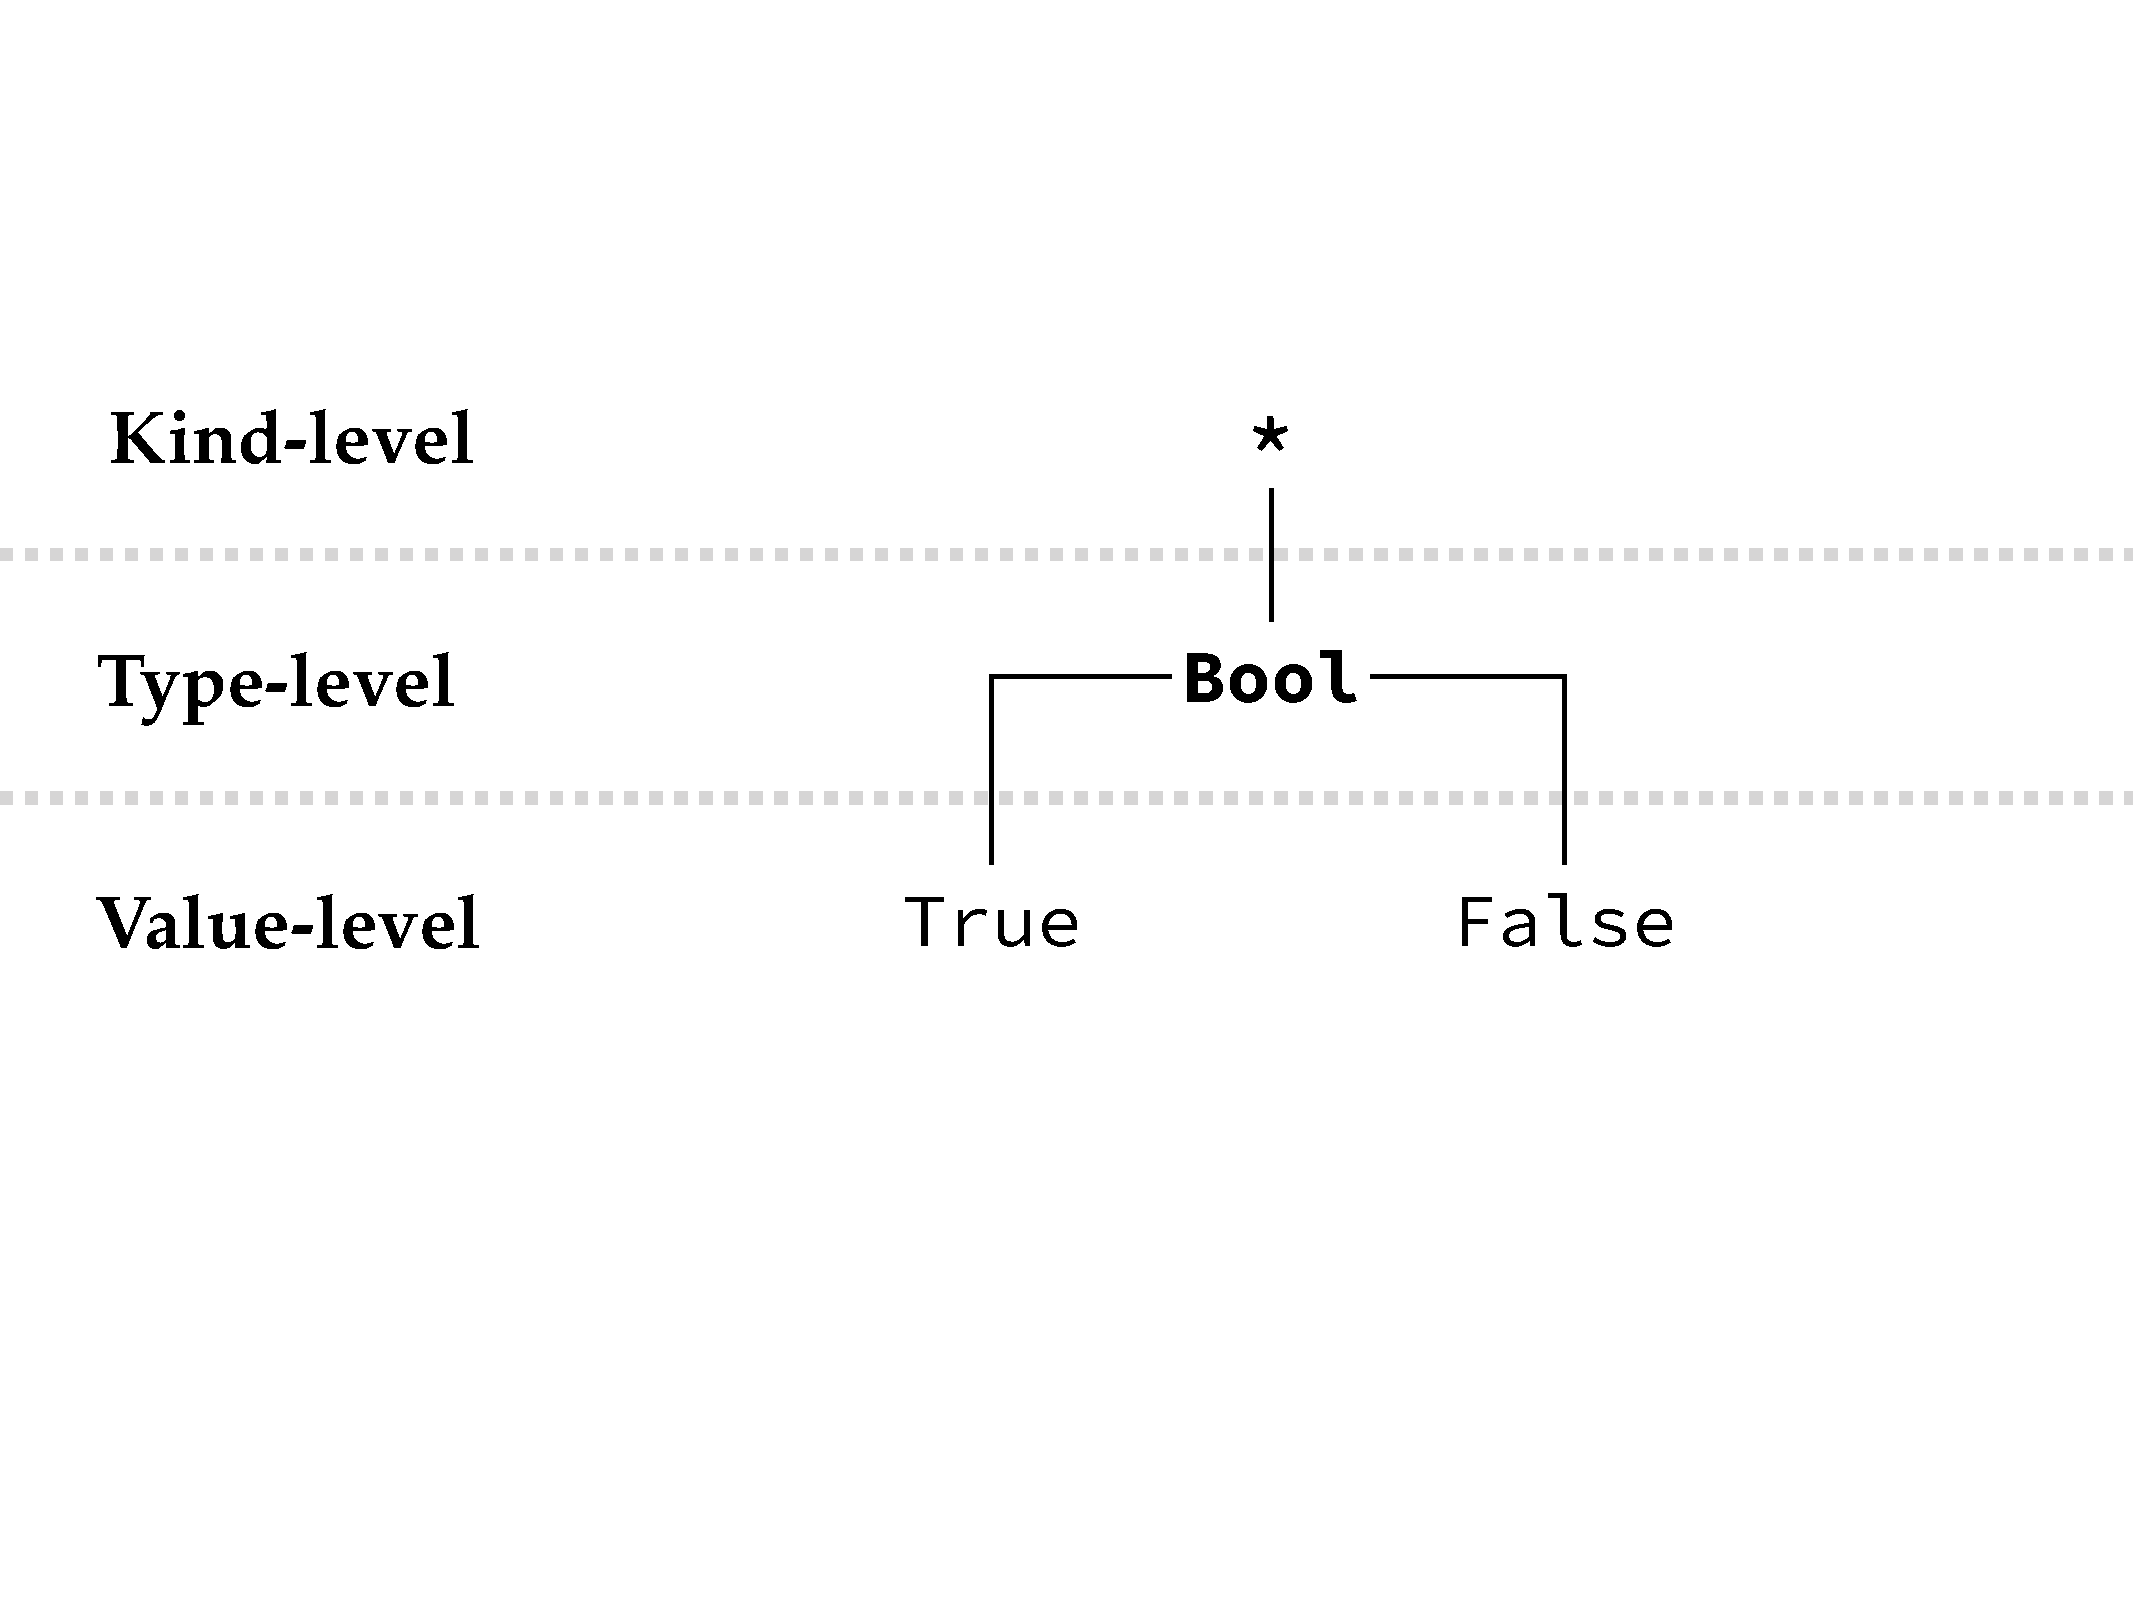
\includegraphics[clip, trim=0cm 10cm 0cm 6cm, width=1.00\textwidth]{labs/bool.pdf}

That is, \haskellIn{Bool} is a type and there are two values of this type: \haskellIn{True} and \haskellIn{False}. As an ordinary type, it is of kind \haskellIn{*} (read as \emph{type}). With \texttt{\small -XDataKinds} (\emph{i.e.} type promotion) enabled, the \texttt{\small Bool} type is automatically promoted to its own kind and its data constructors, \haskellIn{True} and \haskellIn{False}, are automatically promoted to types of that kind, all \emph{in addition to the above}. We can visualise this as:

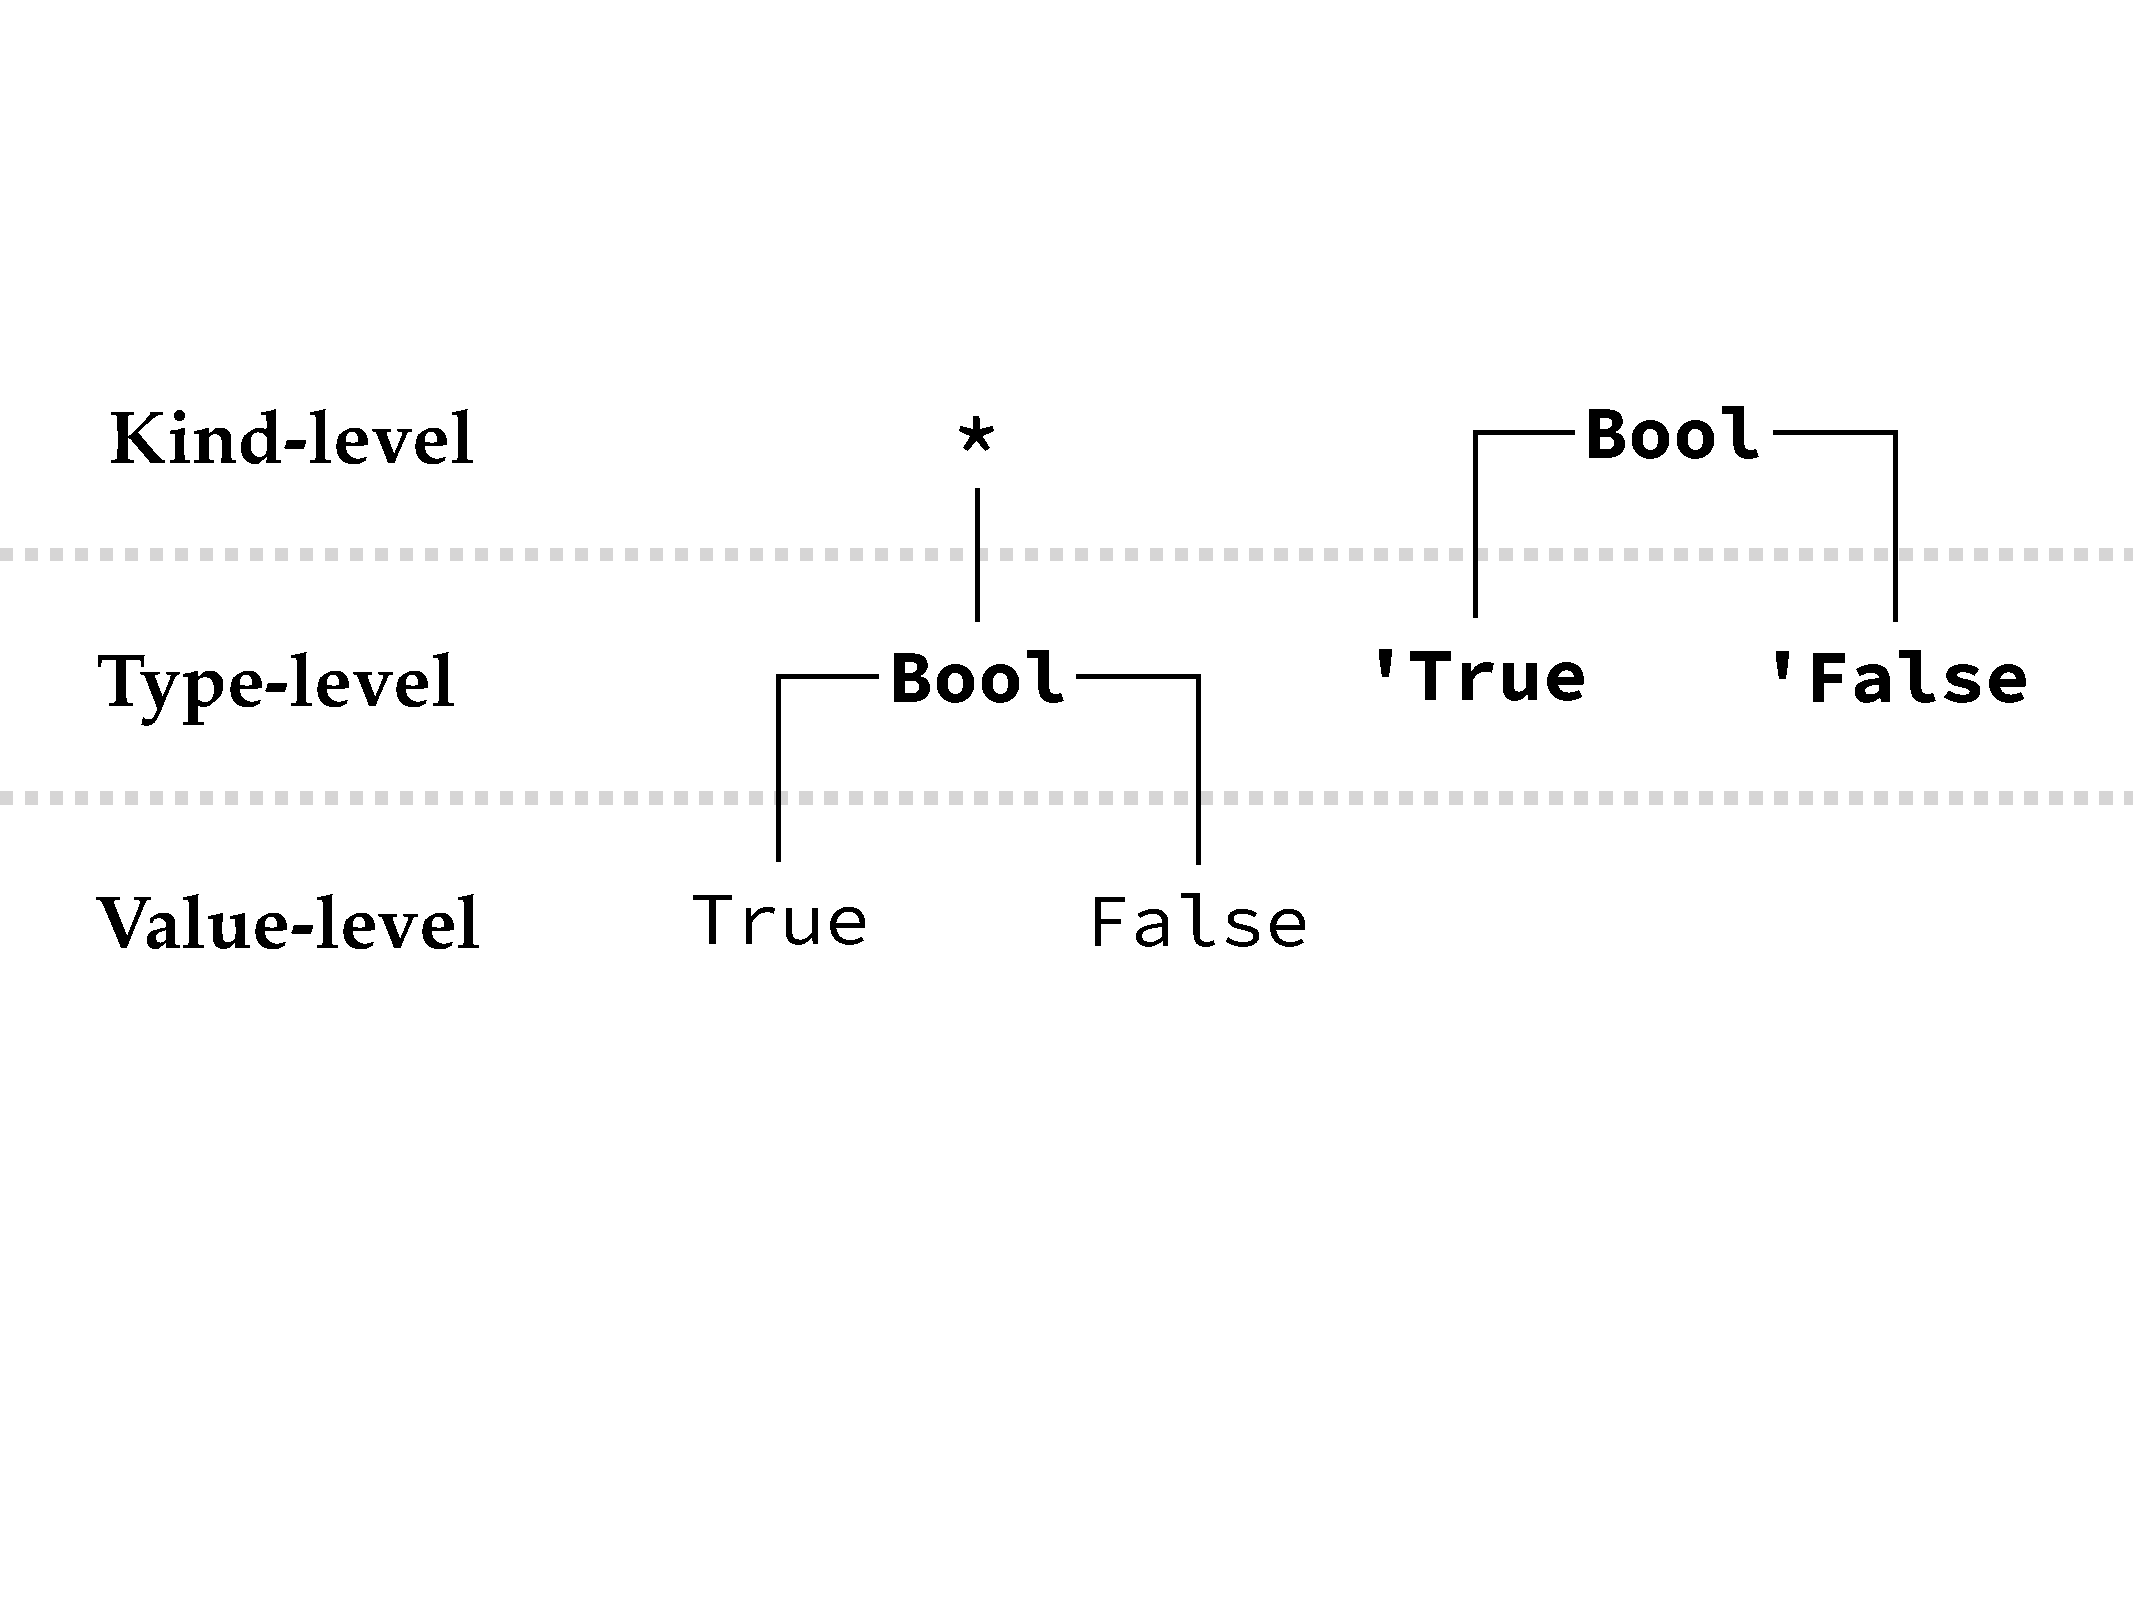
\includegraphics[clip, trim=0cm 10cm 0cm 6cm, width=1.00\textwidth]{labs/bool-promoted.pdf}

In addition to the \haskellIn{Bool} type with its \haskellIn{True} and \haskellIn{False} constructors, we now have a kind that is also named \haskellIn{Bool}. There are two types of kind \haskellIn{Bool}: \haskellIn{'True} and \haskellIn{'False}. Run the following commands in the REPL to validate what we have described:
\begin{itemize}
	\item \texttt{\small :k Bool} 
	\item \texttt{\small :t True} 
	\item \texttt{\small :k 'True} 
	\item \texttt{\small :k True} 
\end{itemize}
Note that the last two commands are the same. Because types and values are different namespaces, we can often just write \haskellIn{True} instead of \haskellIn{'True} to refer to the type named \haskellIn{True}. However, to avoid ambiguity it is always good practice to explicitly include the \texttt{'}.

\taskLine

\task{GHC also provides type-level lists out-of-the-box for us when \texttt{\small -XDataKinds} is enabled. Try the following in the REPL:}
\begin{itemize}
	\item \texttt{\small :k []}
	\item \texttt{\small :t (:)}
	\item \texttt{\small :t []}
	\item \texttt{\small :k '[]}
	\item \texttt{\small :k (:)}
	\item \texttt{\small :k Int :~'[]}
\end{itemize} \newpage  
\section{Type-level programming}
\topics{Kinds, phantom types, GADTs, singleton types, pattern matching with GADTs, data type promotion, closed and open type families.}

This final set of exercises is all about type-level programming. The skeleton code can be obtained as usual with the following command:
\begin{minted}{bash}
$ git clone https://github.com/fpclass/lab-tlp
\end{minted}

\faBook~\emph{Further reading}: for more examples of type-level programming in action, \emph{Fun with type functions} \citep{kiselyov2010fun} is a good read. The first two chapters of \emph{Giving Haskell a promotion} \citep{yorgey2012giving} give an overview of key type-level programming techniques in Haskell.

\taskLine 

\task{Define a closed type family \texttt{\small Not} which performs boolean negation at the type-level. Check that your solution works correctly by running \texttt{\small stack test} as usual.}

\task{Once defined, you should be able to use the REPL commands to infer the types and kinds of your new definition. Try the following:}
\begin{itemize}
	\item \texttt{\small :k Not}
	\item \texttt{\small :k Not True}
	\item \texttt{\small :kind!~Not True}
\end{itemize}

\taskLine

\task{Modify the definition of \texttt{\small SBool} to define a singleton type for booleans. This type should have kind \texttt{\small Bool -> *} and two constructors named \haskellIn{STrue} and \haskellIn{SFalse} with appropriate types. Once you have defined this type, verify in the REPL that the type has the correct kind and that the constructors have the correct types. The unit tests will also ensure that \haskellIn{STrue} and \haskellIn{SFalse} have the correct types.}

\task{Having a singleton type for booleans is useful as we can now keep track of the value of a boolean variable at the type-level and therefore at compile-time. This allows us to define functions of types such as:}
\begin{minted}{haskell}
inot :: SBool b -> SBool (Not b)
\end{minted}
That is, given a value of type \texttt{\small SBool b} where \texttt{\small b} is a type of kind \texttt{\small Bool} corresponding to the value, \haskellIn{inot} should return a boolean whose value is the negation of \texttt{\small b}. Implement this function now so that we get the expected behaviour:
\begin{minted}{haskell}
inot STrue  ==> SFalse 
inot SFalse ==> STrue
\end{minted}
While this is not very interesting on the term-level, what happens if you ask the REPL for the types of these expressions?
\begin{itemize}
	\item \texttt{\small :t inot STrue}
	\item \texttt{\small :t inot SFalse}
\end{itemize}

\task{Could you define similar functions for other boolean operations, such as \haskellIn{and}?}

\task{Given a type that is known at compile-time, we may wish to convert it to a corresponding value on the value-level. This process is in general known as \emph{reification} and can be accomplished with the help of a suitable type class. We now want to do this for type-level booleans. You are already given the definition of a suitable type class, named \haskellIn{KnownBool}. Implement suitable instances of this type class so that \haskellIn{boolVal} can be used in the following ways:}
\begin{minted}{haskell}
boolVal (Proxy :: Proxy True)  ==> True
boolVal (Proxy :: Proxy False) ==> False
\end{minted}

\taskLine 

The aim of this last part of these exercises is to implement \emph{heterogeneous lists} in Haskell. The ``ordinary'' lists that we have come across in Haskell are homogeneous: that is, every element has the same type. For example, the following is a valid list in Haskell because all elements have the same type:
\begin{minted}{haskell}
[4,8,15,16,23,42] :: [Int]
\end{minted}  
However, the following is not a valid list in Haskell because its elements have different types:
\begin{minted}{haskell}
[True,"Duck"] -- not well typed
\end{minted} 
This is because lists in Haskell need to be parametrised by the element type: the list type constructor \texttt{\small []} has kind \haskellIn{* -> *}. The definition of lists assumes that every element has that type:
\begin{minted}{haskell}
[]  :: [a]
(:) :: a -> [a] -> [a]
\end{minted} 
In order to implement lists where the elements can have different types, we need to be able to parametrise a list by the types of all of its elements. In other words, we need a type constructor of kind \texttt{\small [*] -> *}. That is, a type constructor which requires a list of types as argument.

\task{With the help of type-level lists, complete the definition of \texttt{\small HList} so that it has two constructors: \haskellIn{HNil} which represents an empty, heterogeneous list and \haskellIn{HCons} which adds an element to a heterogeneous list. Some examples of what should work successfully in the REPL once you are done:}
\begin{minted}{haskell}
*Lab> :t HNil
HNil :: HList '[]
*Lab> :t HCons True HNil
HCons True HNil :: HList '[Bool]
*Lab> :t HCons 4 (HCons True HNil)
HCons 4 (HCons True HNil) :: Num a => HList '[a, Bool]
\end{minted}

\task{Implement the \haskellIn{hhead} function, which should work just like \haskellIn{head} does on ordinary lists, but for heterogeneous lists.}

\task{Define suitable instances of the \haskellIn{Show} type class so that we can use the \haskellIn{show} function on heterogeneous lists. For example:}
\begin{minted}{haskell}
show HNil                          ==> "[]"
show (HCons 4 HNil)                ==> "4 : []"
show (HCons "cake" (HCons 4 HNil)) ==> "\"cake\" : 4 : []"
\end{minted}
Once implemented, all tests should pass.

\task{(\emph{Difficult}) Replace your instances of the \haskellIn{Show} type class that you wrote for the previous exercise with new ones so that the \haskellIn{show} function on heterogeneous lists works as follows instead:}
\begin{minted}{haskell}
show HNil                          ==> "[]"
show (HCons 4 HNil)                ==> "[4]"
show (HCons "cake" (HCons 4 HNil)) ==> "[\"cake\", 4]"
\end{minted}
\emph{Hint}: Constraint kinds\footnote{\url{http://blog.omega-prime.co.uk/2011/09/10/constraint-kinds-for-ghc/}} may help you solve this task.
  


% submission details
\newcommand{\deadlineOneTime}{noon}
\newcommand{\deadlineOneDate}{6 February 2020}
\newcommand{\submissionOneURL}{https://tabula.warwick.ac.uk/coursework/submission/0d913a74-f440-4f72-afd4-d84cb6ada99a}

%\renewcommand{\instructions}{Due at \emph{\deadlineTime} on \emph{\deadlineDate}.}


\cleardoublepage
\chapter{Coursework I}

\section{The Large Arithmetic Collider}

The goal of this coursework is to implement a Haskell program which can solve a challenging combinatorial game, which we refer to as the \emph{large arithmetic collider}. The game is based on a grid containing mathematical operations. To explain how it works, let us start with a simple example. Consider the following 4x1 sized grid containing the operations $+31$, $-26$, $-14$, $-1$ from left to right:
\begin{center}
	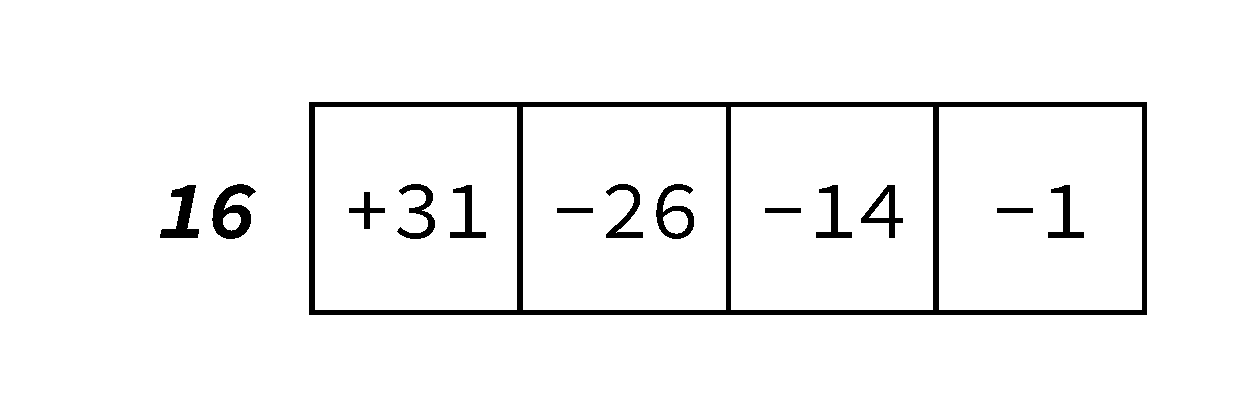
\includegraphics[scale=0.4,trim=0 30 0 30]{cswk/lac1.pdf}
\end{center}
You will also note that this row is annotated with the number $16$. The goal is to determine which of the operations contained in the cells result in that number when applied from left to right, starting with $0$. The solution for this simple example is shown below, where the cells containing operations that can be used to obtain the target number are shaded in grey:
\begin{center}
	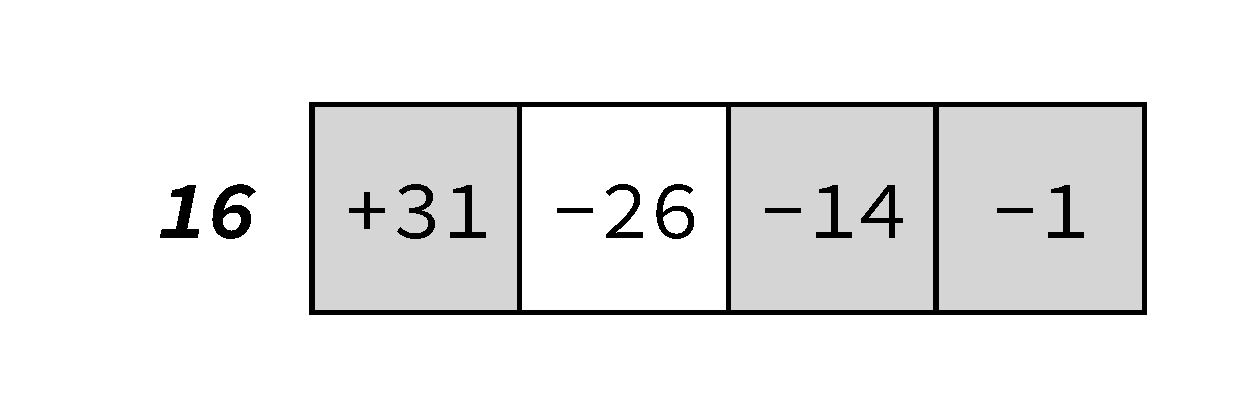
\includegraphics[scale=0.4,trim=0 30 0 30]{cswk/lac1s.pdf}
\end{center}
As we can easily see here, this is a solution because $0+31-14-1=16$. Since there are 4 cells in this example and each cell can either be used or not, there are $2^4=16$ possible configurations to explore here when searching for a solution. Although there is only one solution for this example, in general each grid may have more than one solution or, indeed, no solution. 

You may notice that we are talking about a ``grid'', but have only shown a single row to illustrate the basic game mechanics so far. A more realistic grid is shown below:
\begin{center}
	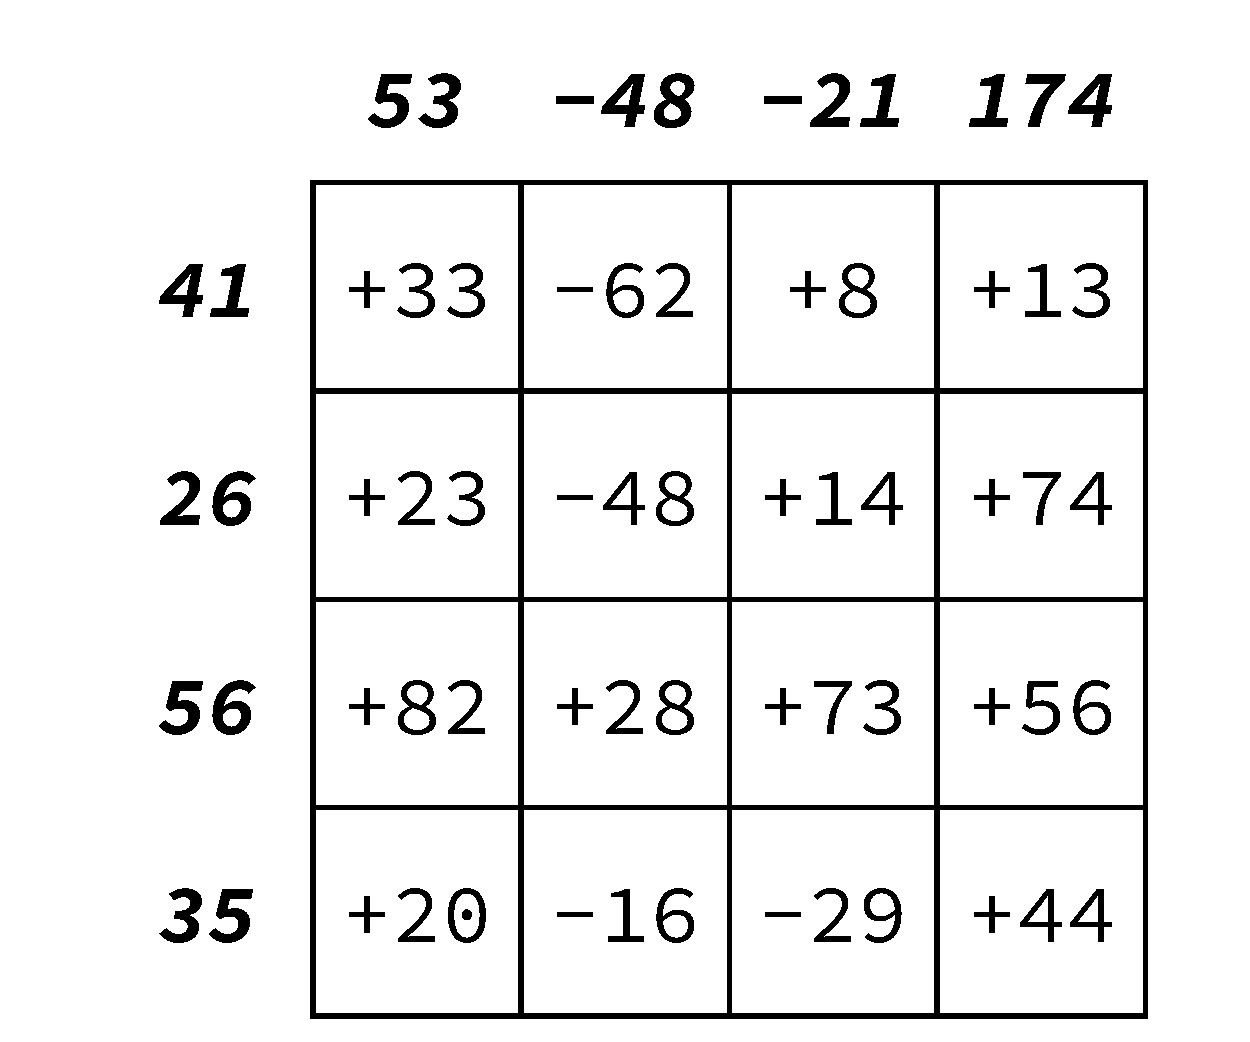
\includegraphics[scale=0.4,trim=0 30 0 30]{cswk/lac2.pdf}
\end{center}
As we can see, every row and every column is annotated with a target number. We must find which operations to use so that each row results in its target number as described in the previous example, but so that each column also results in its target number. The rules for columns are the same as for rows: we start with 0 and apply each active operation from top to bottom. The solution for this grid is shown below:
\begin{center}
	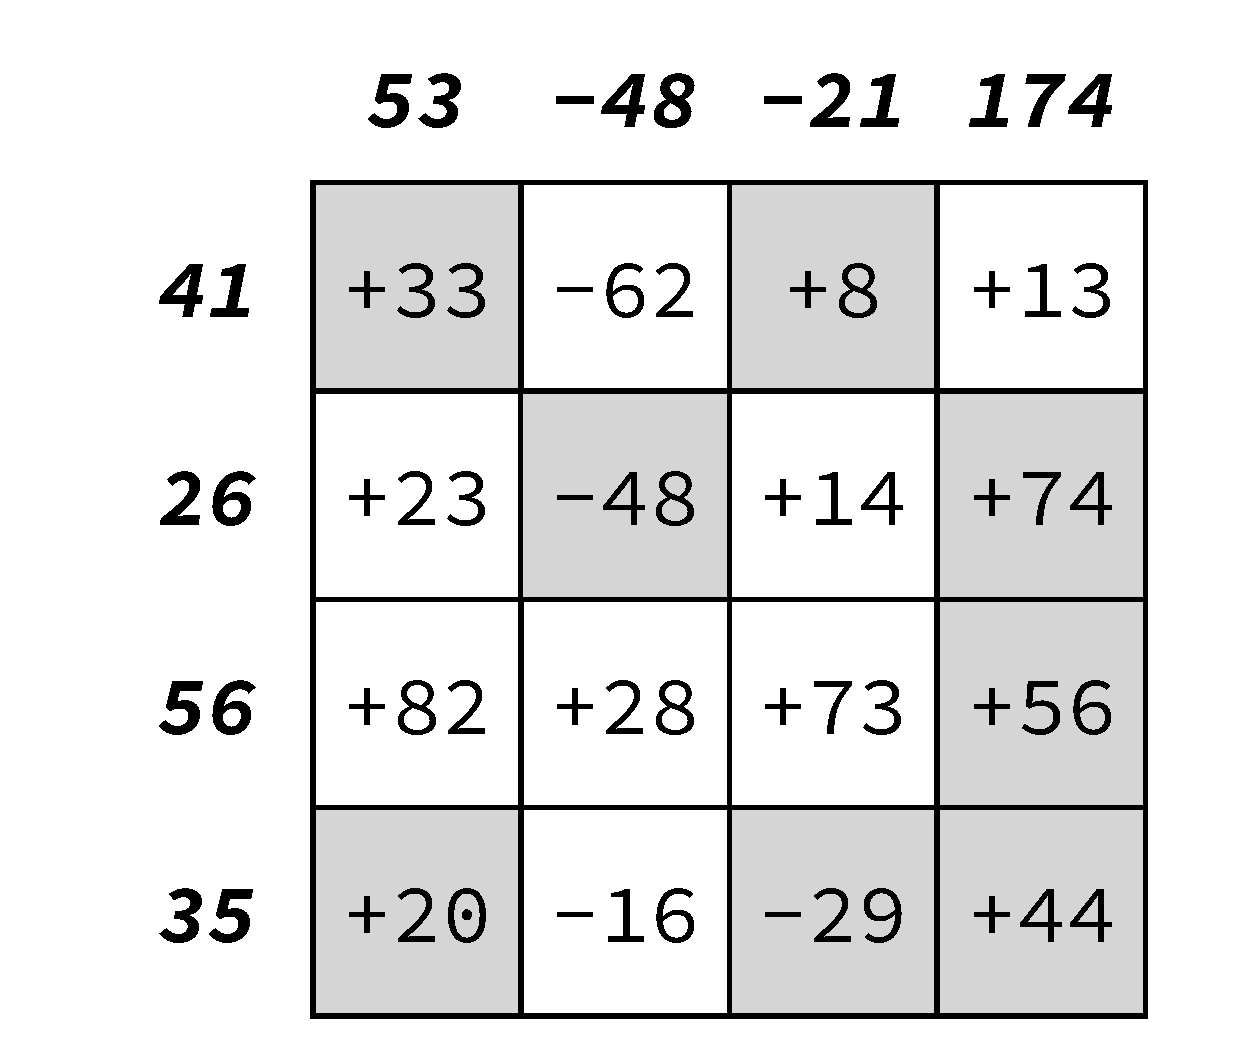
\includegraphics[scale=0.4,trim=0 30 0 30]{cswk/lac2c.pdf}
\end{center} 
Finding a solution for this grid is significantly more difficult. There are $4 \times 4 = 16$ cells and the number of possible configurations to explore is therefore $2^{16} = 65535$. Fortunately, this is still fairly simple for a computer to solve. At this point, you are encouraged to skip ahead to \Cref{sec:cswk1-getting-started} and implement the code required to solve grids using these mechanics.

\subsection{Advanced gameplay}

To further increase the difficulty of the game, there is one more game mechanic: the grids we have encountered so far can all be solved as they are, but we can also consider grids where rows or columns must be \emph{rotated} first. For example, consider the following grid:
\begin{center}
	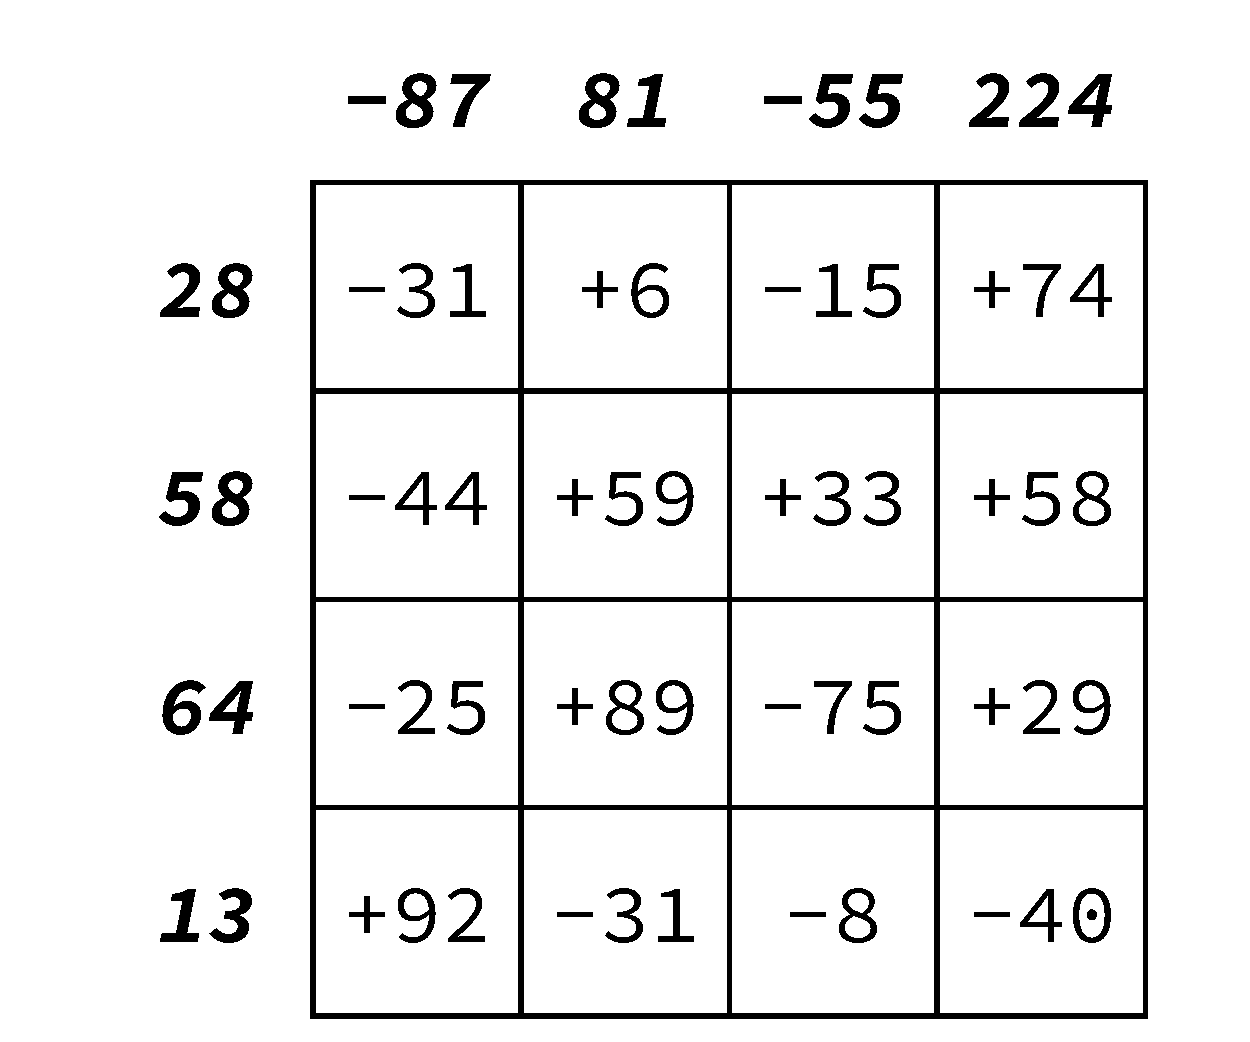
\includegraphics[scale=0.4,trim=0 30 0 30]{cswk/lac3.pdf}
\end{center}
This grid has no solutions as it is. However, we can find solutions if we change the layout of the cells by rotating some of the rows or columns. The rules for this are as follows: we can rotate one row or column at a time. We refer to this as one \emph{move}. Grids which can be solved without any rotations are solved in 0 moves. If a grid cannot be solved in 0 moves, then our goal is to try and solve it in as few moves as possible. For the example shown above, we can solve it in one move by rotating the last row of the grid:
\begin{center}
	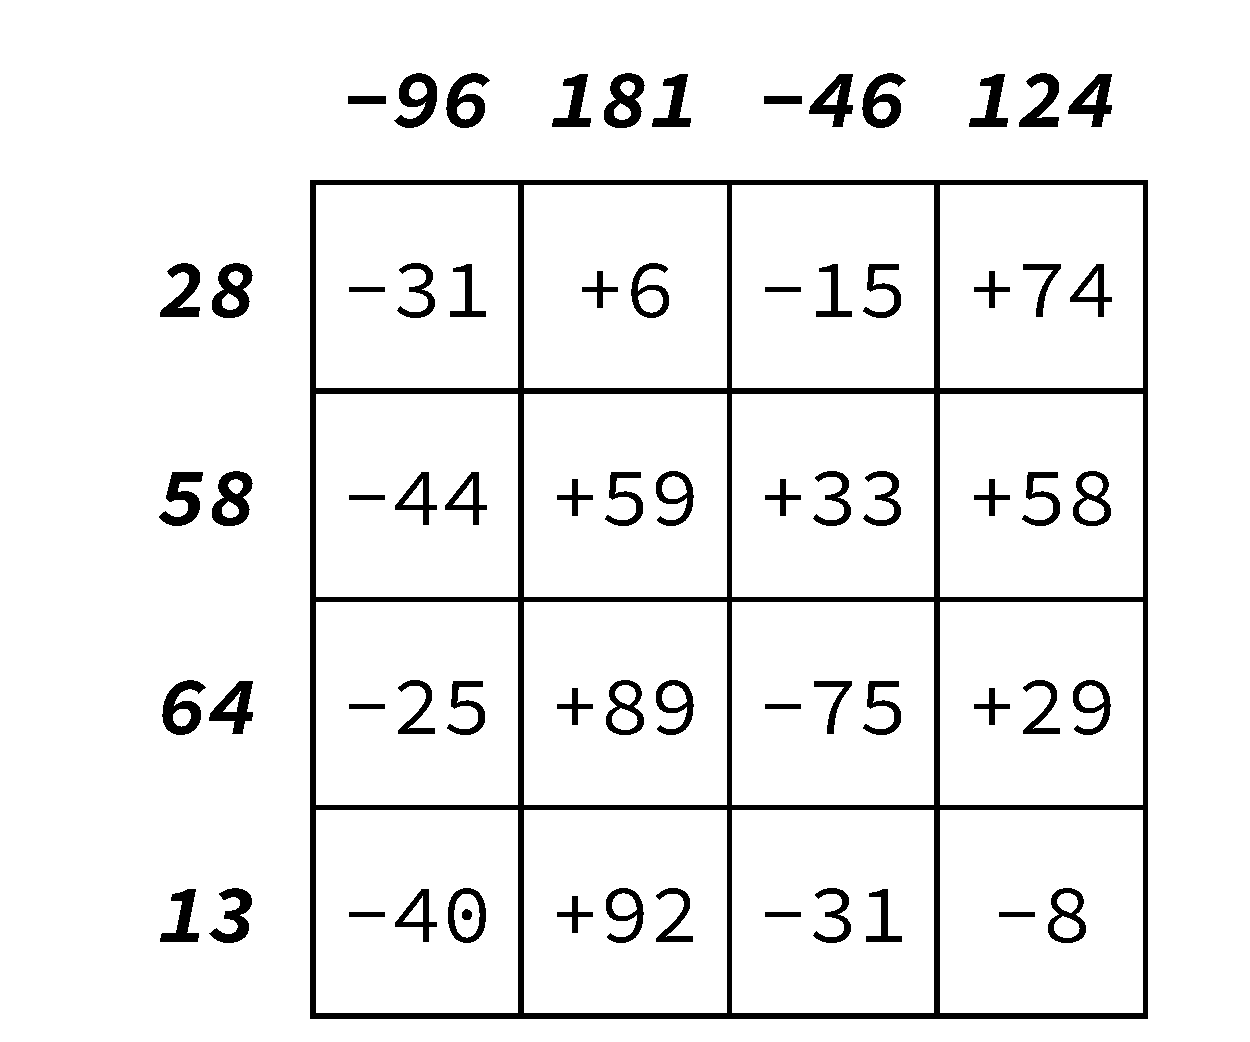
\includegraphics[scale=0.4,trim=0 30 0 30]{cswk/lac3r.pdf}
\end{center}
Rotations are always performed from left to right or top to bottom. Therefore, there are always $\mathit{rows}+\mathit{columns}$-many possible rotations at any given step. With the last rotated as shown, there is now a solution for the resulting grid:
\begin{center}
	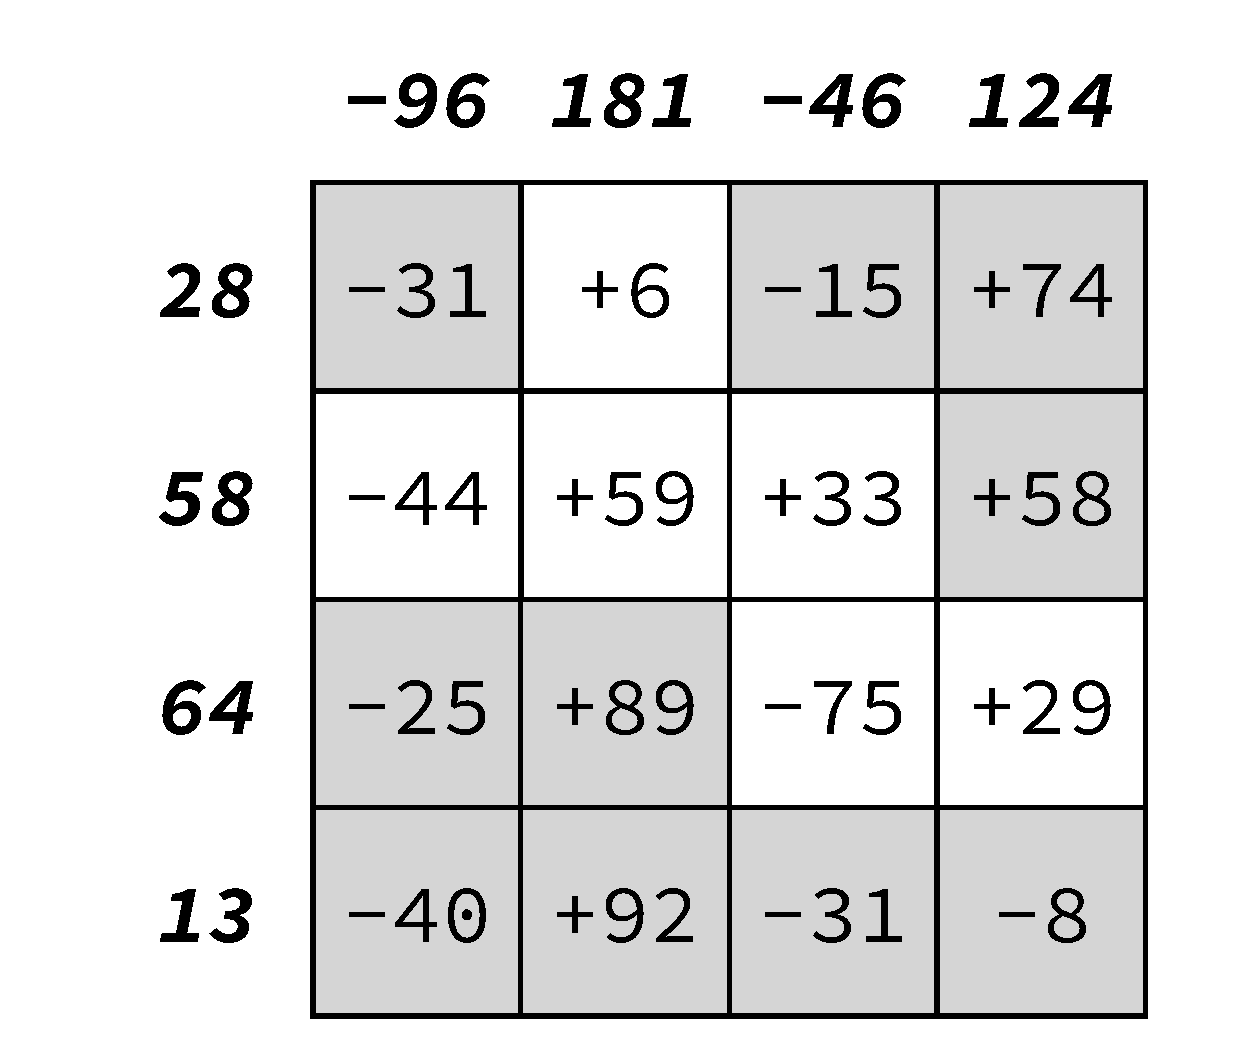
\includegraphics[scale=0.4,trim=0 30 0 30]{cswk/lac3s.pdf}
\end{center}
Finding a solution for a grid that cannot be solved in 0 moves is much harder than finding solutions for one that can be solved in 0 moves. In principle, we can use rotations to create an arbitrary arrangement of cells in the grid, thus leaving us with $(\mathit{rows} \times \mathit{columns})!$ many arrangements of cells. That means that for a $4 \times 4$ sized grid as the one shown above, there are $20,922,789,888,000$ many arrangements of cells. Each cell can then either be used or not, so for each of those arrangements there are $2^{4 \times 4}$ possible solutions, leaving us with a total state space of $(4 \times 4)! \times 2^{4 \times 4}$ many possible solutions. However, just finding a solution in itself does not tell us how to get there from the grid we start with, so a smarter approach is needed...

%-----------------------------------------------------------

\section{Getting started}
\label{sec:cswk1-getting-started}

In order to get started with the coursework, you need to get hold of the skeleton code and ensure that it compiles successfully on your machine. 

\subsection{Obtaining the skeleton code}

There are three different ways in which you can obtain the skeleton code for this coursework. All of them are explained below alongside their various advantages and disadvantages:

\paragraph{Option A: Private fork} By following the GitHub Classroom link below, you can create a private fork of our git repository with the skeleton code. This requires a GitHub account, but has the advantage that you have your own private copy of our repository on GitHub that you can write to. That would allow then you to work easily share your work between machines in the labs and at home:
\begin{center}
	\url{https://classroom.github.com/a/94xWYjXL}
\end{center}
Once you have accepted the assignment, you can then clone your fork of the skeleton code to your machine with the usual \bashIn{git clone} command where \texttt{\small [username]} is your GitHub username:
\begin{minted}{bash}
$ git clone https://github.com/fpclass/1920-cswk1-[username]
\end{minted}
\paragraph{Option B: Clone} If you do not wish to create a GitHub account or host a copy of your repository there, then you could instead just clone our repository with:
\begin{minted}{bash}
$ git clone https://github.com/fpclass/large-arithmetic-collider
\end{minted}
You will be able to \bashIn{git commit} changes to your local copy of the repository, but you will not be able to \bashIn{git push} them. This is sufficient if you are only planning to work on the coursework from one place (\emph{e.g.} only the lab machines but not your personal computer).

\paragraph{Option C: Archive} If GitHub should be unavailable or you do not have \bashIn{git} installed your machine, you can download a \texttt{\small .zip} file with the skeleton code from the module website.

\subsection{Working with the skeleton code}

You may wish to verify that the code compiles and that all tests fail by entering the \texttt{\small large-arithmetic-collider} directory that was created and running \texttt{\small stack test}:
\begin{minted}{text}
$ cd large-arithmetic-collider
$ stack test
\end{minted}
Running \texttt{\small stack test} will compile your code, run a bunch of unit tests on it, and give you a rough indication of how complete your solution is (the more tests pass, the more complete it is). %Running \bashIn{stack bench} will run a set of benchmarks on your code. 
You can also use \bashIn{stack build} to just compile your code and then \texttt{\small stack exec collider} to run the program. Alternatively, you can run \bashIn{stack repl} to load up the REPL, which is useful for debugging.

The skeleton code contains a bunch of files, most of which you do not need to touch. The most important file is \texttt{\small src/Game.hs} which contains the definitions you will need to complete in order to implement the game. There are some definitions to get you started. Firstly, the arithmetic operations that may be contained in cells of the grids are represented as an algebraic data type where each constructor represent one type of operation:
\begin{minted}{haskell}
data Action 
  = Add Int 
  | Sub Int 
\end{minted}
Cells themselves are also represented as an algebraic data type comprised of a boolean value indicating whether the cell is enabled or not and an \haskellIn{Action} value representing the arithmetic operation contained in the cell:
\begin{minted}{haskell}
data Cell = Cell Bool Action
\end{minted}
Rows are comprised of a target number and a list of cells:
\begin{minted}{haskell}
data Row = Row Int [Cell]
\end{minted}
Finally, grids are comprised of a list of target numbers for all the columns and a list of all the rows in the grid:
\begin{minted}{haskell}
data Grid = Grid [Int] [Row]
\end{minted}

%-----------------------------------------------------------

%\section{Solving complex grids}



%-----------------------------------------------------------

\section{Task}

Complete all definitions in \texttt{\small src/Game.hs} so that the game works as described above. The following function stubs in \texttt{\small src/Game.hs}  need to be implemented:

\begin{enumerate}
	\item \haskellIn{eval :: Action -> Int -> Int}\\
	This function should apply an arithmetic operation represented by an \haskellIn{Action} value to an accumulator and return the result. For example, \haskellIn{eval (Add 5) 10} should evaluate to \haskellIn{15}.
	
	\item \haskellIn{apply :: Cell -> Int -> Int}\\
	This function should apply the arithmetic operation contained in a \haskellIn{Cell} value to an accumulator and return the result if the cell is enabled. For example, \haskellIn{eval (Cell True (Add 5) 10} should evaluate to \haskellIn{15} while \haskellIn{eval (Cell False (Add 5) 10} should evaluate to \haskellIn{10}.
	
	\item \haskellIn{result :: [Cell] -> Int}\\
	This function should determine the result of evaluating all the enabled arithmetic operations in a list of cells, starting with $0$. For example, evaluating \haskellIn{result [Cell True (Add 3), Cell False (Add 5)]} should result in \haskellIn{3}.
	
	\item \haskellIn{solveRow :: Row -> [Row]}\\
	This function should find all solutions for a given row.
	
	\item \haskellIn{solve :: Grid -> [Grid]}\\
	This function should find all solutions for a given grid, without rotating any rows or columns. If there are no solutions, an empty list should be returned.
	
	\item \haskellIn{rotations :: Grid -> [Grid]}\\
	Given a grid, this function should return a list of grids containing all possible ways to rotate the input grid. This means the resulting list should normally have $\mathit{rows} + \mathit{columns}$ many elements.
	
	\item \haskellIn{steps :: Grid -> [Grid]}\\
	If a grid cannot be solved without rotating it, this function should return a list of grids representing the shortest sequence of rotations which lead to a solution. I.e. the last grid in the list should be the solution and each grid should differ from the previous by exactly one rotation.
\end{enumerate}

%-----------------------------------------------------------

\section{Originality \& academic practice}

This coursework is an individual assignment and the work you submit must be entirely your own work. Students are expected to be familiar with the departmental Student Handbook as well as applicable university regulations. The ``Cheating and Plagiarism'' section on the handbook page about coursework is particularly relevant:
\begin{center}\small
	\url{https://warwick.ac.uk/fac/sci/dcs/teaching/handbook/coursework/}
\end{center}
Examples of what is not acceptable in the context of this assignment include, but are not limited to, the following:
\begin{itemize}
	\item Collaborating with others, for example by sharing code, looking at other people's code, or discussing implementation details such as which functions you used to implement a particular definition. 
	
	\item Copying or adapting code from web sources such as Stack Overflow, GitHub, etc. without attribution. This includes taking code written in other programming languages and translating it to Haskell. You may do this if you include a correct attribution to the source in e.g. a comment in your file, but note that you can only be awarded marks for work you have done yourself. 
\end{itemize}

%-----------------------------------------------------------

\section{Marking \& submission}

This coursework is worth 15\% of the overall module mark. It will be marked out of 100\% as follows:
\begin{itemize}
	\item 20\% for \emph{correctness and documented understanding (basic grids)}. You gain full marks here if all parts of the coursework required to solve basic grids (up to and including the \haskellIn{solve} function) been attempted and are correct. You may use \texttt{\small stack test} as a rough indication for whether this is the case, but there are some things the unit tests do not test for, so you should play the game and ensure that everything works as described. You should also document your code with comments and explain how it works. You gain full marks if all code is documented and explained sufficiently well so that someone who is unfamiliar with your code can understand it.
	
	\item 20\% for \emph{correctness and documented understanding (advanced grids)}. You gain full marks here if all parts of the coursework required to solve advanced grids (the \haskellIn{steps} function) been attempted and are correct. You may use \texttt{\small stack test} as a rough indication for whether this is the case, but there are some things the unit tests do not test for, so you should play the game and ensure that everything works as described. You should also document your code with comments and explain how it works. You gain full marks if all code is documented and explained sufficiently well so that someone who is unfamiliar with your code can understand it.
	
	\item 20\% for \emph{elegance}. Definitions should be concise and readable, new functions should be introduced where needed, existing library functions used when applicable, etc.
	 
	\item 20\% for \emph{performance and efficiency}. To do well here, you need to use sensible data structures and your functions should perform as little redundant computation as possible. In your comments, you must also discuss what you have done to test your solution's performance and what you have tried to improve it. %You can test performance by running \bashIn{stack bench} on different versions of your code to see how they compare.  
	
	\item 20\% for \emph{improvements and extensions}. This is an opportunity for you to demonstrate creativity and advanced understanding. You could achieve this in many different ways, such as adding additional unit tests, functionality, improved algorithms, etc. You may wish to modify \texttt{\small app/Main.hs} as well as other source files or even add new ones. You could also prove some properties about your game on paper. The amount of marks awarded will depend on the complexity and creativity of your extension(s) and improvement(s).
\end{itemize}
Submit a \texttt{\small .zip} or \texttt{\small .tar.gz} archive of the whole, completed project (not just \texttt{\small Game.hs}) through Tabula by \deadlineOneTime\ on \deadlineOneDate:
\begin{center} 
	\url{\submissionOneURL}
\end{center}


% submission details
\newcommand{\deadlineTwoTime}{noon}
\newcommand{\deadlineTwoDate}{18 March 2021}
\newcommand{\submissionTwoURL}{https://tabula.warwick.ac.uk/coursework/submission/ac09b7de-5e75-45f9-87e9-ab847d96a001}
\newcommand{\classroomTwoURL}{https://classroom.github.com/a/aW9z1Yip}

%\renewcommand{\instructions}{Due at \emph{\deadlineTime} on \emph{\deadlineDate}.}

\cleardoublepage
\chapter{Coursework II}

\section{Scratch clone}

Scratch\footnote{\url{https://scratch.mit.edu/}} is a visual programming language designed to teach programming to children in a fun and graphical way. Programs in Scratch are built by arranging blocks that correspond to different syntactic constructs and connecting them like puzzle pieces. The tool is free to use so you can give it a go if you want! To give you an idea of what it looks like, here is a screenshot of Pac-Man built in Scratch running on a Raspberry Pi:

\begin{center}
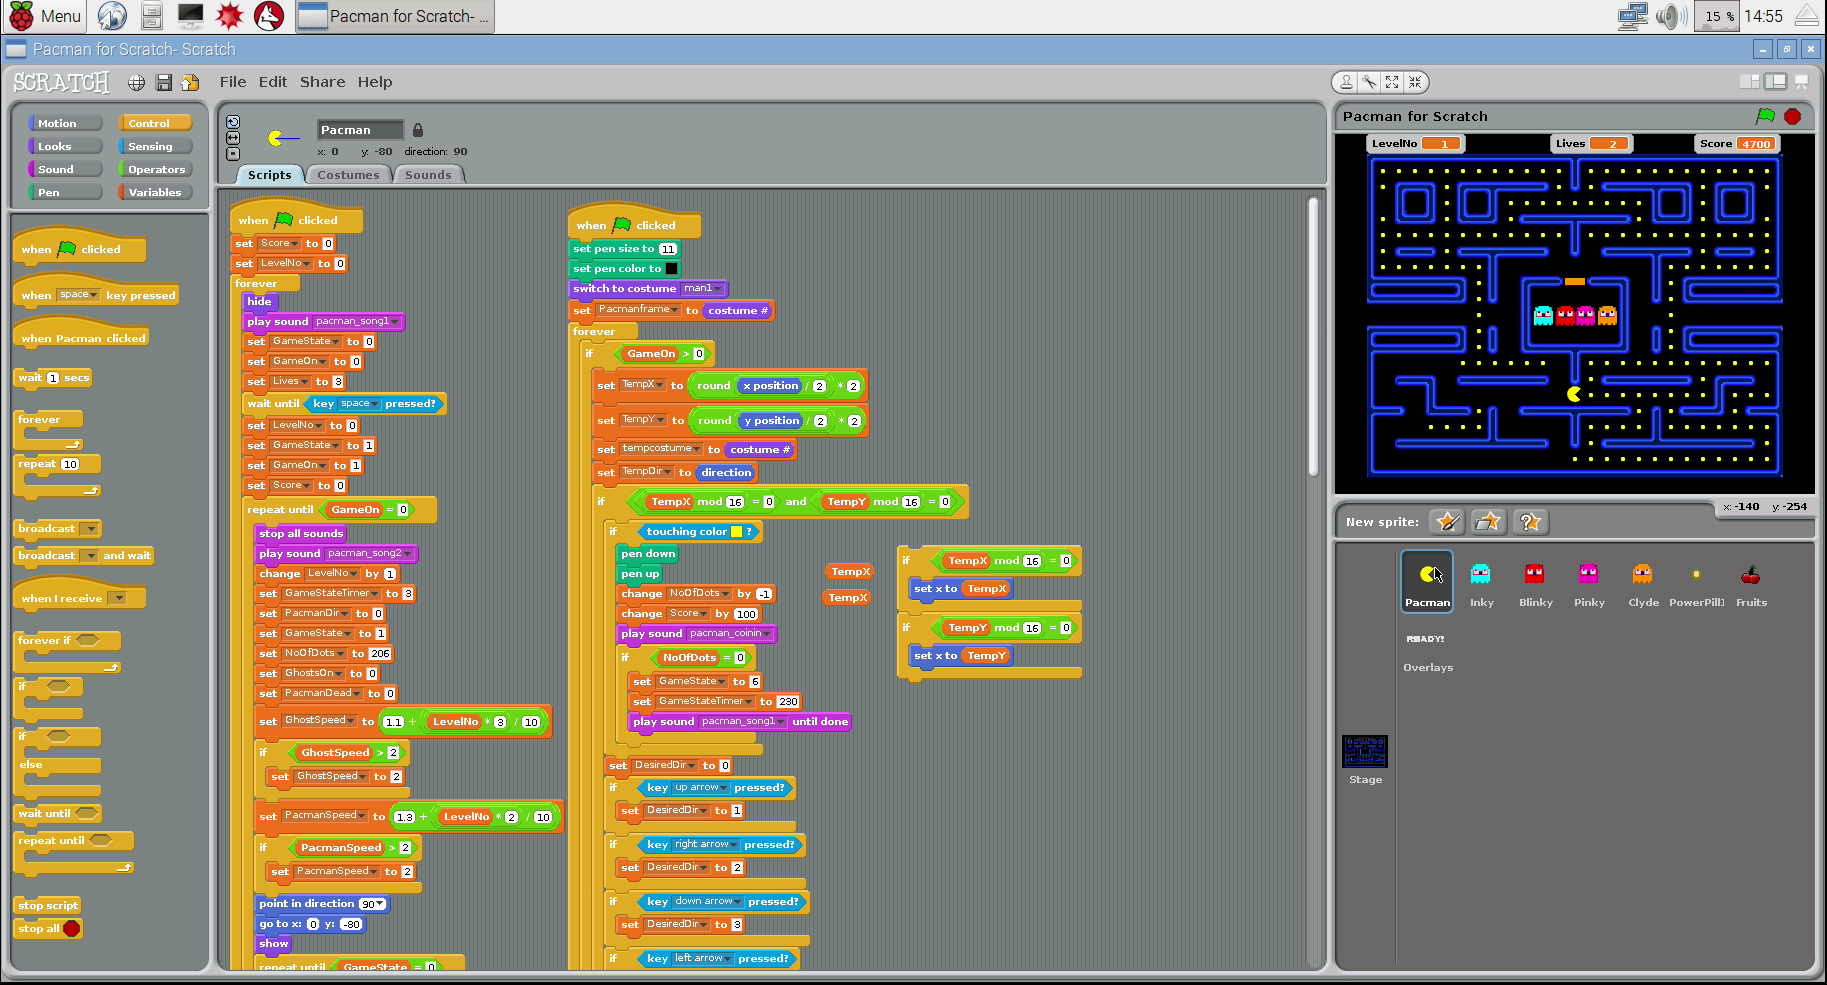
\includegraphics[width=390px]{cswk/scratch_rpi.png}
\end{center}

The goal of this coursework is to implement a simple clone of Scratch. Our clone will consist of two components:
\begin{enumerate}
    \item A web-based interface which allows users to construct simple programs visually. This is written in JavaScript and is already implemented for you.
    \item A Haskell program which handles the evaluation of such programs. This is partially implemented and you will have to finish it.
\end{enumerate}
Your task is to complete the part of the Haskell program responsible for evaluating programs -- in other words, you have to write an \emph{interpreter}.

An interpreter is a program which, given some representation of a program as argument, evaluates it. To illustrate this idea, a Haskell implementation of an interpreter for a simple expression language is shown below:
\begin{minted}{haskell}
data Expr = Val Int | Add Expr Expr 

eval :: Expr -> Int
eval (Val n)   = n
eval (Add l r) = eval l + eval r
\end{minted}
Expressions in the language represented by \haskellIn{Expr} consist of the addition operator and integer values. The \haskellIn{eval} function is the interpreter for this language, which determines the value of a given expression.

\section{Getting started}

In order to get started with the coursework, you need to get hold of the skeleton code and ensure that it compiles successfully. 

\subsection{Obtaining the skeleton code}

There are three different ways in which you can obtain the skeleton code for this coursework, which are all explained below alongside their advantages and disadvantages:

\paragraph{Option A: Private fork} By following the GitHub Classroom link below, you can create a private fork of our git repository with the skeleton code. This requires a GitHub account, but has the advantage that you have your own private copy of our repository on GitHub that you can write to. That would allow then you to work easily share your work between machines in the labs and at home:
\begin{center}
	\url{\classroomTwoURL}
\end{center}
Once you have accepted the assignment, you can then clone your fork of the skeleton code to your machine with the usual \bashIn{git clone} command where \texttt{\small [username]} is your GitHub username:
\begin{minted}{bash}
$ git clone https://github.com/fpclass/2021-cswk2-[username]
\end{minted}

\paragraph{Option B: Clone} If you do not wish to create a GitHub account or host a copy of your repository there, then you could instead just clone our repository with:
\begin{minted}{bash}
$ git clone https://github.com/fpclass/scratch-clone
\end{minted}
You will be able to \bashIn{git commit} changes to your local copy of the repository, but you will not be able to \bashIn{git push} them. This is sufficient if you are only planning to work on the coursework from one place (\emph{e.g.} only the lab machines but not your personal computer).

\paragraph{Option C: Archive} If GitHub should be unavailable or you do not have \bashIn{git} installed your machine, you can download a \texttt{\small .zip} file with the skeleton code from the module website.

\subsection{Working with the skeleton code}

The code should compile out of the box. You can test this by running:
\begin{minted}{bash}
$ stack build
\end{minted}
To start the program, you should run the following:
\begin{minted}{text}
$ stack exec scratch-clone
Starting web server...
Started. Press any key to quit.
\end{minted}
In order to view the user interface, open your web browser and navigate to\footnote{If, for whatever reason, port 8000 is unavailable on your machine, you can change this by modifying the definition of \haskellIn{main} in \texttt{\small src/Main.hs}.}:
\begin{center}
\url{http://localhost:8000/}
\end{center}
You can drag together programs using building blocks from the toolbox on the left. However, if you click ``Evaluate'' at the top right corner of the screen, you will get an error since the interpreter is not yet implemented.

The skeleton code contains a bunch of files, most of which you do not need to touch initially. The most important file is \texttt{\small src/Interpreter.hs} which contains the definitions you will need to complete to get the interpreter to work. There are some definitions to get you started. A program's initial memory is represented as a list of pairs. Each pair represents one variable, consisting of a name of type \haskellIn{String} and a value of type \haskellIn{Int}:
\begin{minted}{haskell}
type Memory = [(String, Int)]
\end{minted}
It is possible for things to go wrong when interpreting a program. There are two sorts of errors which may occur. These are represented by the following data type:
\begin{minted}{haskell}
data Err = DivByZeroError | UninitialisedMemory String
\end{minted}
The types representing the language itself are defined in \texttt{\small src/Language.hs}. You should have a look at this file yourself, but an overview of the most important types is below. A program is a list of statements:
\begin{minted}{haskell}
type Program = [Stmt]
\end{minted}
There are three different forms of statements: 
\begin{minted}{haskell}
data Stmt = AssignStmt String Expr
          | IfStmt Expr [Stmt] [(Expr,[Stmt])] [Stmt]
          | RepeatStmt Expr [Stmt]
\end{minted}
Assignments, represented by the \haskellIn{AssignStmt} constructor, consists of the name of the variable that we are assigning a value to and the expression whose value we should assign to the variable. 

If statements, represented by the \haskellIn{IfStmt}, are more complicated. The first expression is the condition of the ``if'' clause. The list of statements which follows is the code that should be run if the condition is true. The list of pairs of expressions and lists of statements represent ``if else'' clauses. Finally, the last list of statements represents the ``else'' clause.

Repeat statements, represented by the \haskellIn{RepeatStmt} constructor, consist of an expression which determines how many times the repeat loop should be executed and a list of statements which represent the body of the repeat statement.

There are also three forms of expressions:
\begin{minted}{haskell}
data Expr = ValE Int
          | VarE String
          | BinOpE Op Expr Expr
\end{minted}
The \haskellIn{ValE} constructor represents integer values, the \haskellIn{VarE} constructor represents variables, and the \haskellIn{BinOpE} constructor generalises binary operators. The \haskellIn{Op} data type in \texttt{\small src/Language.hs} enumerates all available operators.

\section{Task}

Complete the definition of the \haskellIn{interpret} function in \texttt{\small src/Interpreter.hs} so that all values of type \haskellIn{Program} can be evaluated correctly according to the rules described below. Programs are sequences of statements and should be evaluated in the order in which they are given. We illustrate all rules for the language with screenshots of the GUI and the expected results:

\begin{center}
	\begin{longtable}[t]{|c|p{5cm}|}
		\hline 
		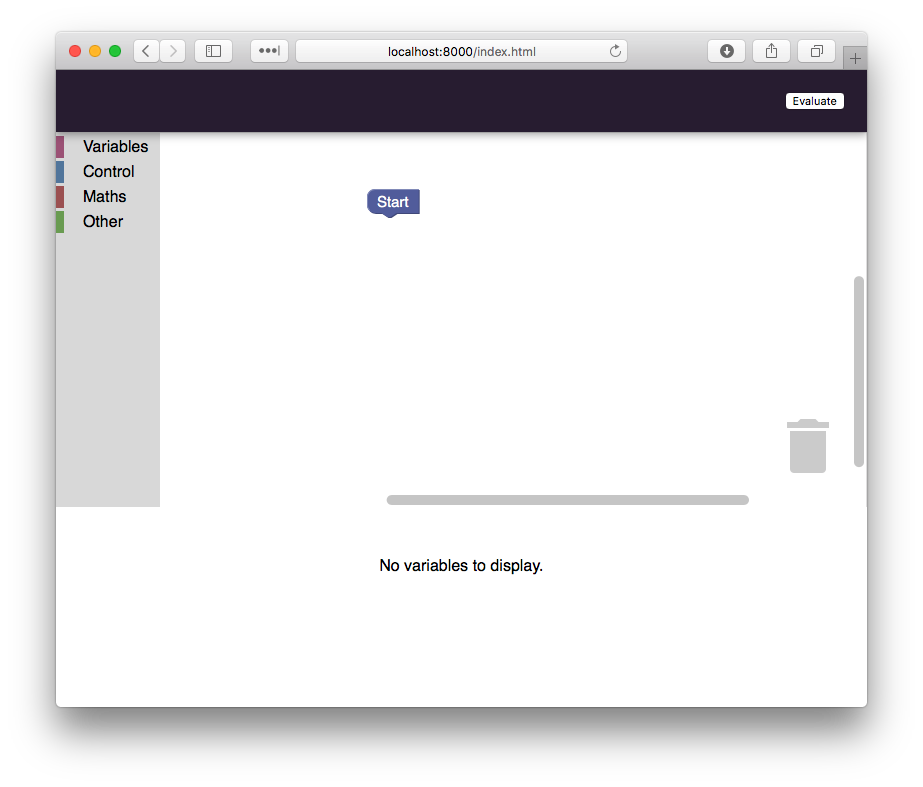
\includegraphics[align=t,width=250px]{cswk/0-empty.png} & 
		If the program is empty as shown in the screenshot, the initial contents of the memory should be returned. \\ \hline 
		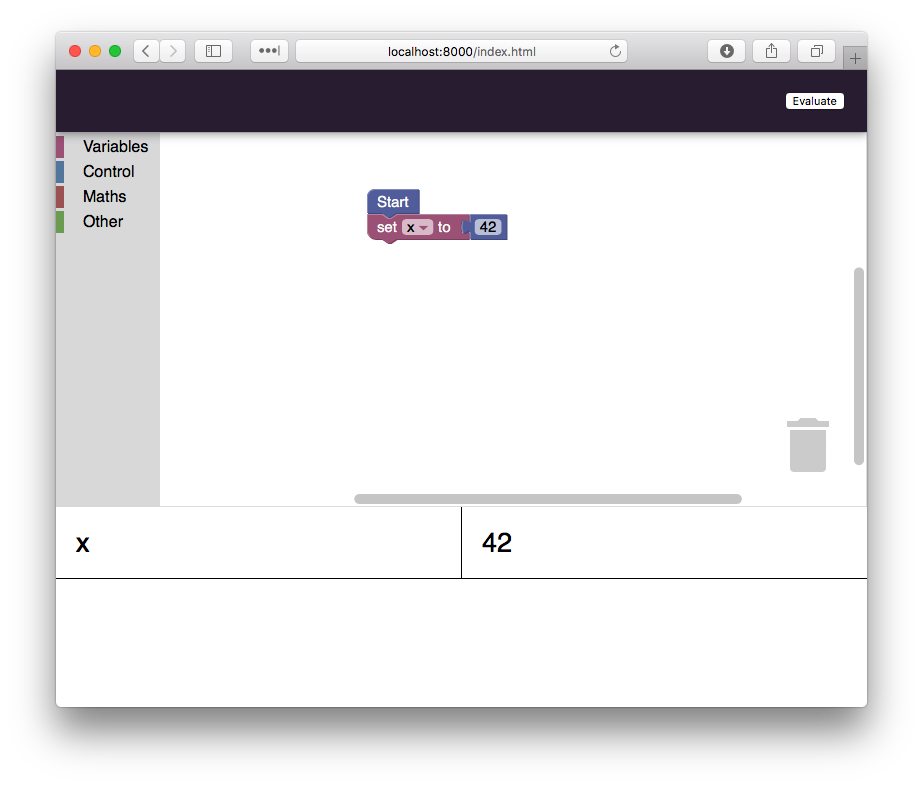
\includegraphics[align=t,width=250px]{cswk/1-assignment.png} & 
		Assignment statements should update the memory to the value of their expression. \\ \hline 
		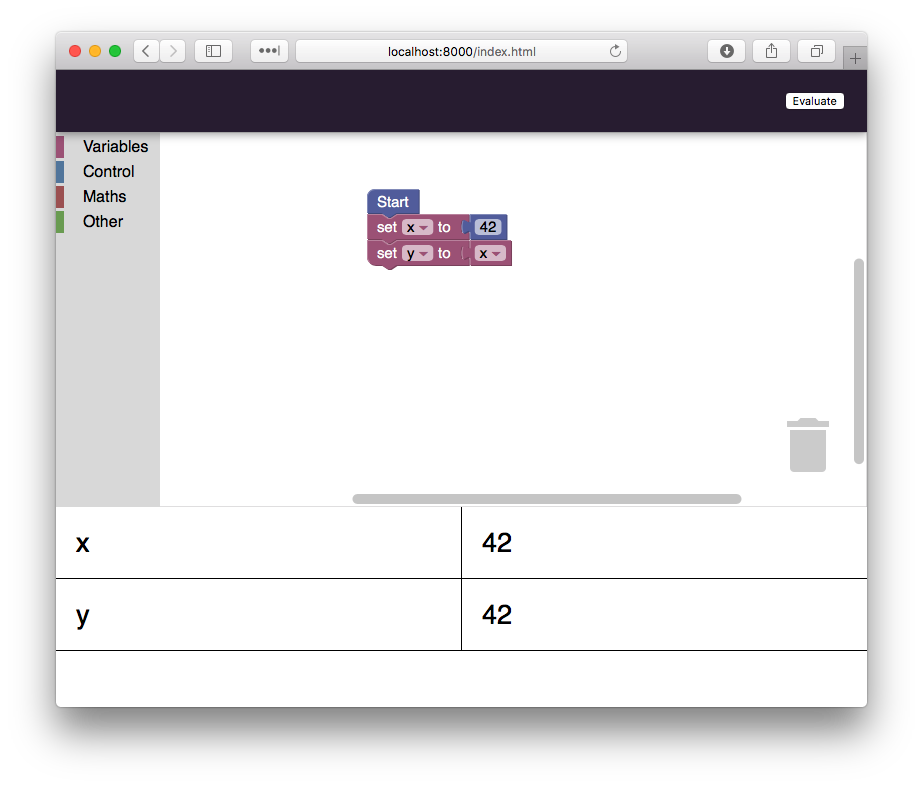
\includegraphics[align=t,width=250px]{cswk/2-loading.png} &
		If a variable occurs in an expression, the corresponding value should be loaded from memory. \\ \hline 
		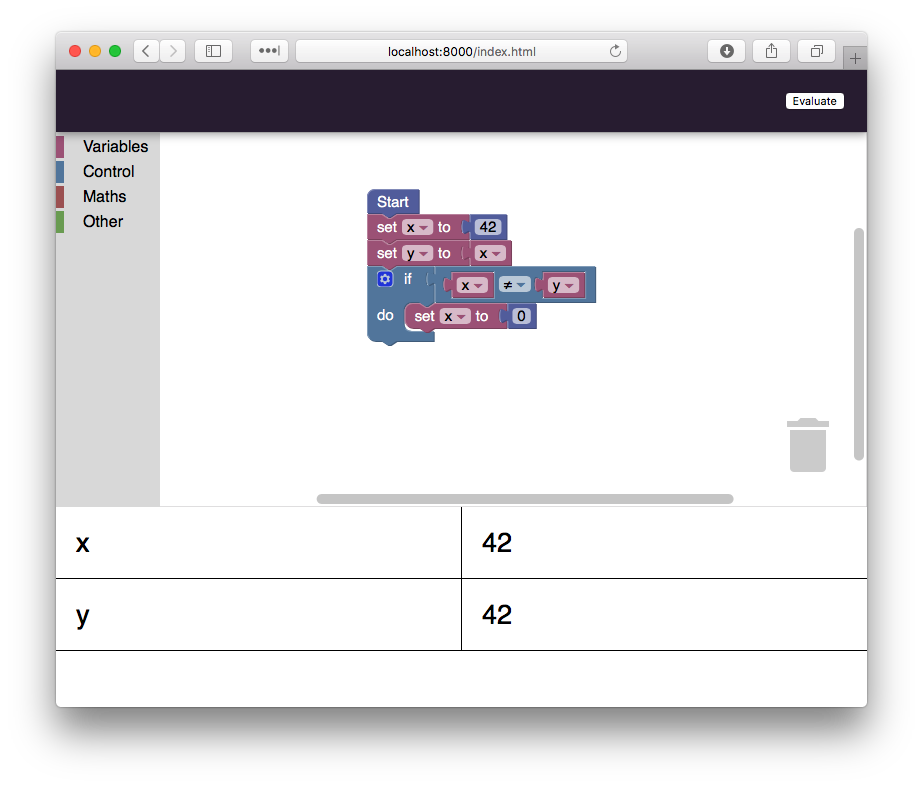
\includegraphics[align=t,width=250px]{cswk/3-if.png} &
		If the condition of an if statement is true (\emph{i.e.} any non-zero value), then the body of the if clause should be executed. \\ \hline
		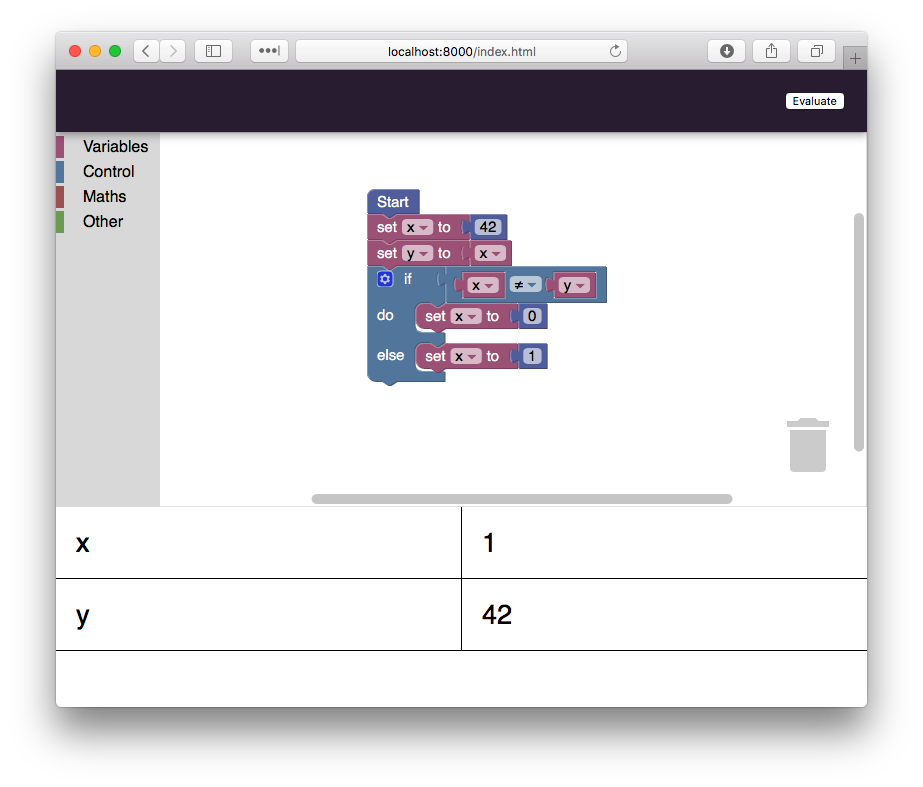
\includegraphics[align=t,width=250px]{cswk/4-else.png} &
		If the condition of an if statement is false (\emph{i.e.} it evaluates to zero), then the body of the else clause should be executed. \\ \hline 
		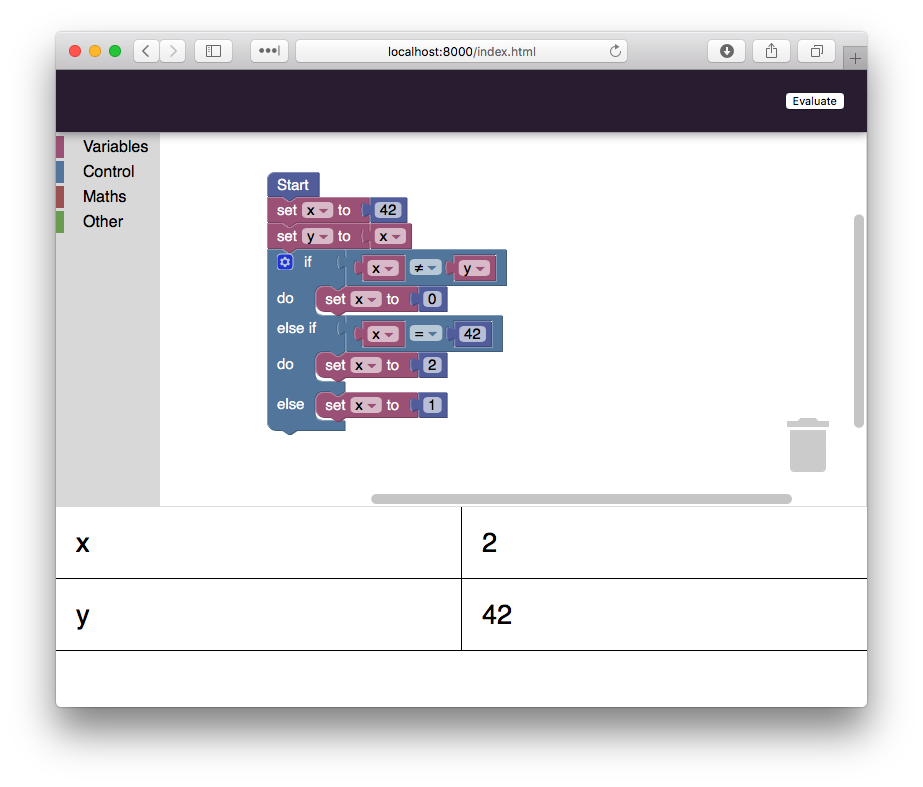
\includegraphics[align=t,width=250px]{cswk/5-ifelse.png} &
		If there are if else clauses present, their conditions should be checked in order after that of the main if clause. If one of them is true, then the corresponding body should be executed. \\ \hline
		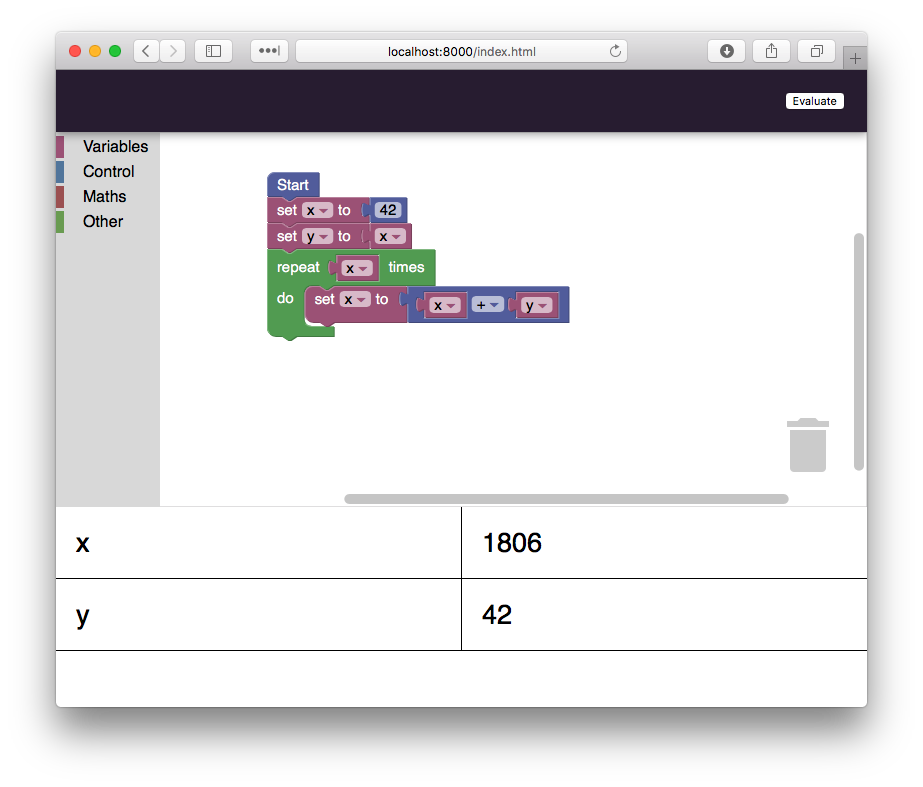
\includegraphics[align=t,width=250px]{cswk/6-repeat.png} &
		Repeat statements evaluate an expression to determine how many times they should run. The body of the repeat statement is then executed that many times. \\ \hline 
		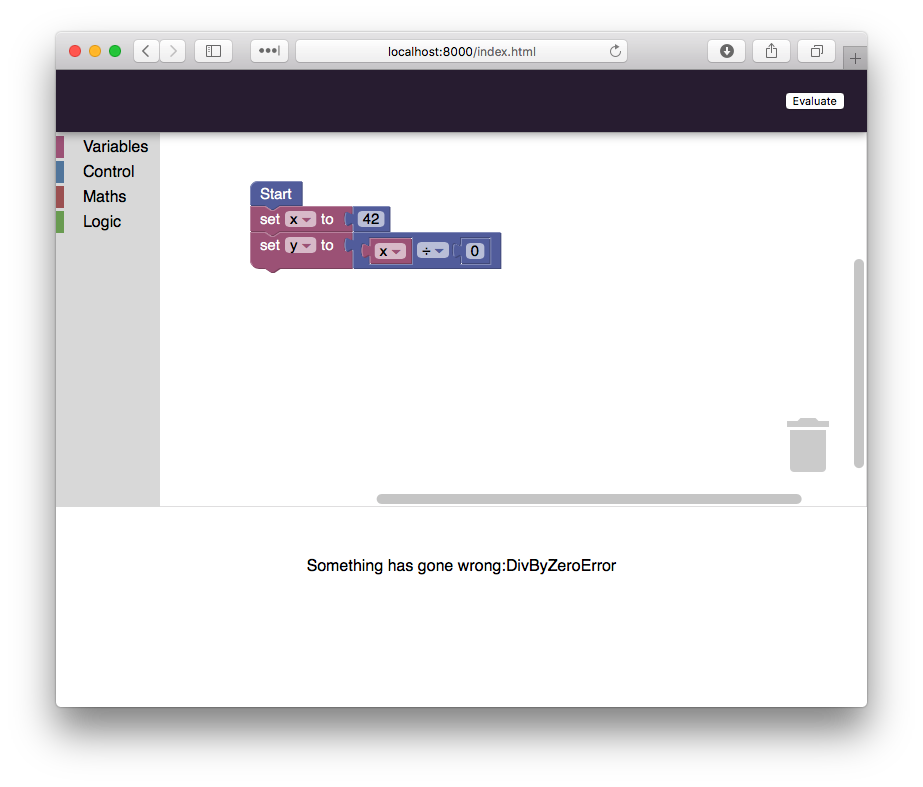
\includegraphics[align=t,width=250px]{cswk/7-divbyzero.png} &
		If a division by zero is attempted, the corresponding error should be returned. \emph{I.e.} \haskellIn{Left DivByZeroError} \\ \hline
	\end{longtable}
\end{center}
There are some details to look out for:
\begin{itemize}
	\item Internally, logic operators should evaluate to $0$ if false or a non-zero value if true. All numeric values other than $0$ should be treated as true.
	\item If an attempt is made to read from a variable which is not in the memory, then the corresponding error should be returned.
	\item Expressions can be nested arbitrarily deep and expressions of arbitrary complexity may appear in any place where expressions are expected.
	\item Errors can arise almost anywhere and should be propagated properly.
\end{itemize}

Running \texttt{\small stack test} will give you a rough indication of how complete your solution is. Running \bashIn{stack bench} will benchmark your code.

%-----------------------------------------------------------

\section{Originality \& academic practice}

This coursework is an individual assignment and the work you submit must be entirely your own work. Students are expected to be familiar with the departmental Student Handbook as well as applicable university regulations. The ``Cheating and Plagiarism'' section on the handbook page about coursework is particularly relevant:
\begin{center}\small
	\url{https://warwick.ac.uk/fac/sci/dcs/teaching/handbook/coursework/}
\end{center}
Examples of what is not acceptable in the context of this assignment include, but are not limited to, the following:
\begin{itemize}
	\item Collaborating with others, for example by sharing code, looking at other people's code, or discussing implementation details such as which functions you used to implement a particular definition. 
	
	\item Copying or adapting code from web sources such as Stack Overflow, GitHub, etc. without attribution. This includes taking code written in other programming languages and translating it to Haskell. You may do this if you include a correct attribution to the source in e.g. a comment in your file, but note that you can only be awarded marks for work you have done yourself. 
\end{itemize}

\section{Marking \& submission}

This coursework is worth 25\% of the overall module mark. It will be marked out of 100\% as follows:
\begin{itemize}
	\item 20\% for \emph{correctness}. You gain full marks here if all parts of the coursework have been attempted and are correct. You may use \bashIn{stack test} as a rough indication for whether this is the case, but there are some things the unit tests do not test for, so you should construct programs in the scratch clone and ensure that everything works as described.
	
	\item 20\% for \emph{documented understanding}. You should document your code with comments and explain how it works. You gain full marks if all code is documented and explained sufficiently well so that someone who is unfamiliar with your code can understand it.
	
	\item 20\% for \emph{elegance}. Definitions should be concise and readable, new functions should be introduced where needed, existing library functions used when applicable, monads used where possible, etc. 
	
	\item 20\% for \emph{performance and efficiency}. To do well here, you need to use sensible data structures and your functions should perform as little redundant computation as possible. In your comments, you must also discuss what you have done to test your solution's performance and what you have tried to improve it. You can test performance by running \bashIn{stack bench} on different versions of your code to see how they compare. 
	
	\item 20\% for \emph{improvements and extensions}. This is an opportunity for you to demonstrate creativity and advanced understanding. You could achieve this in many different ways, such as adding additional unit tests, functionality, improved algorithms, etc. You may wish to modify \texttt{\small exe/Main.hs} as well as other source files or even add new ones. You could also prove some properties about your interpreter on paper. The amount of marks awarded will depend on the complexity and creativity of your extension(s) and improvement(s).
\end{itemize}
Submit a \texttt{\small .zip} or \texttt{\small .tar.gz} archive of the whole, completed project (not just \texttt{\small Interpreter.hs}) through Tabula by \deadlineTwoTime\ on \deadlineTwoDate:

\begin{center} 
\url{\submissionTwoURL}
\end{center}
\cleardoublepage
\chapter{Revision project}

For revision purposes, you may find yourself wishing to tackle a larger Haskell project than those presented by the lab exercises. For this purpose, we have included a past coursework specification in this chapter which you could work on when revising for the exam. This is entirely optional and no marks are available for completion of this project, but it is fully equipped with tests and benchmarks just like the two current coursework projects.


\section{Mastermind}

The aim of this revision project is to implement the board game \emph{Mastermind} in Haskell with the help of some skeleton code. The game is played by exactly two players: a \emph{codemaker} and a \emph{codebreaker}. At the start of the game, the codemaker makes up a code consisting of four coloured pegs. Pegs are also referred to as symbols. For example:
\begin{center}
    Yellow, Green, Green, Blue
\end{center}
Each colour (symbol) may be used any number of times in the code, as long as the code has no more than four pegs. There are six colours to choose from. The code is \emph{not} disclosed to the codebreaker, whose objective it is to figure out what the code is. The codebreaker does this by repeatedly \emph{guessing} what the code might be. For example, to start the codebreaker might guess the following code at random:
\begin{center}
    Green, Red, Blue, Blue
\end{center}
The codemaker then scores the guess according to the following rules:
\begin{itemize}
    \item For each peg that is in the correct position and has the right colour, the codebreaker scores one coloured marker.
    \item For each peg that is the right colour but in an incorrect position, the codebreaker scores one white marker.
\end{itemize}
For example, for the above guess, the codebreaker would score one white marker for the green peg that is in the wrong position and one coloured marker for the blue peg that is in the right position. The codebreaker does \emph{not} score a white marker for the second blue peg. In other words, at most one point is awarded for each peg in the code. The codebreaker then has to use this score to come up with a new guess for the code, which is then scored again, and so on. Once the codebreaker scores four coloured markers, the game is over and the two players switch roles.

%-----------------------------------------------------------

\subsection{Getting started}

In order to get started with the revision project, you need to get hold of the skeleton code and ensure that it compiles successfully. 

\subsubsection{Obtaining the skeleton code}

To obtain the skeleton code, clone it from GitHub using the following command:
\begin{minted}{bash}
$ git clone https://github.com/fpclass/mastermind
\end{minted}
You will be able to \bashIn{git commit} changes to your local copy of the repository, but you will not be able to \bashIn{git push} them. This is sufficient if you are only planning to work on the coursework from one place (\emph{e.g.} only the lab machines but not your personal computer).

If you wish to fork the repository on GitHub and then clone your fork, feel free to do so.

\subsubsection{Working with the skeleton code}

You may wish to verify that the code compiles and that all tests fail by entering the \texttt{\small mastermind} directory that was created and running \bashIn{stack test}:
\begin{minted}{bash}
$ cd mastermind
$ stack test
\end{minted}
Running \bashIn{stack test} will compile your code, run a bunch of unit tests on it, and give you a rough indication of how complete your solution is (the more tests pass, the more complete it is). Running \bashIn{stack bench} will run a set of benchmarks on your code. You can also use \bashIn{stack build} to just compile your code and then \bashIn{stack exec mastermind} to run the program. Alternatively, you can run \bashIn{stack repl} to load up the REPL, which is useful for debugging.

The skeleton code contains a bunch of files, most of which you do not need to touch. The most important file is \texttt{\small src/Game.hs} which contains the definitions you will need to complete in order to implement the game. There are some definitions to get you started. Firstly, the number of pegs per code is defined as:
\begin{minted}{haskell}
pegs :: Int 
pegs = 4
\end{minted}
Ideally, your solution should still work even if this number is modified. We represent colours using characters from \texttt{a} to \texttt{f} and refer to them as symbols:
\begin{minted}{haskell}
type Symbol = Char 

symbols :: [Symbol]
symbols = ['a'..'f']
\end{minted}
Again, your solution should continue to work even if you modify how many symbols there are and which characters are used to represent them. A code is a list of symbols:
\begin{minted}{haskell}
type Code = [Symbol]
\end{minted}
Codes are scored using coloured and white markers. We define scores to be pairs of integers where the first component of the pair represents the number of coloured markers and the second component represents the number of white markers:
\begin{minted}{haskell}
type Score = (Int, Int)
\end{minted}
A player is either human or a computer:
\begin{minted}{haskell}
data Player = Human | Computer
\end{minted}
The initial codemaker is defined as a constant:
\begin{minted}{haskell}
codemaker :: Player
codemaker = Human
\end{minted}
You can change this value to determine who goes first. Finally, the computer's first guess is defined as:
\begin{minted}{haskell}
firstGuess :: Code 
firstGuess = "aabb"
\end{minted}
You can change this value to change the computer's first guess, but note that values other than \haskellIn{"aabb"} may cause the computer to take more guesses to crack the code.

%-----------------------------------------------------------

\subsection{Five-guess algorithm}

Donald Knuth described an algorithm for Mastermind which, for every code with four pegs, takes a computer no more than five guesses to solve. The algorithm works as follows:

\begin{enumerate}
    \item Let $S$ be a set of all possible codes (\haskellIn{"aaaa"}, \haskellIn{"aaab"}, $\ldots$, \haskellIn{"ffff"}).
    \item Let the first guess be \haskellIn{"aabb"}.
    \item Get the codemaker to score your guess.
    \item If the score has four coloured markers, then the guess was correct.
    \item Otherwise, remove all codes from $S$ which would result in a different score. In other words, we know that the code is somewhere in $S$, so it can only be one which results in the same score for the guess as the one we got from the codemaker. 
    \item Find the next guess as follows. If there is only one code left in $S$, use it. Otherwise, for every possible code $c$ (not just those left in $S$):
    \begin{enumerate}
        \item For each possible score $s$ ($(0,1)$, $(0,2)$, $\ldots$, $(4,0)$):
        \begin{enumerate}
            \item Determine how many other codes would be eliminated from $S$. That is, if the next guess were $c$ and it would get a score of $s$, how many codes would that eliminate from $S$ -- i.e. how many codes with different scores would there be?
        \end{enumerate}
    \end{enumerate}
    Choose the code which is guaranteed to eliminate the most options from $S$. This is calculated in the above step by calculating the minimum of eliminations for each code across all the possible scores it might get.
    In the case of multiple codes producing the same number of guaranteed eliminations, a code which is still a member of $S$ should be picked over one which is not.
    \item Go to Step 3.
\end{enumerate}

%-----------------------------------------------------------

\subsection{Task}

Complete all definitions in \texttt{\small src/Game.hs} so that the game works as described above and that the computer never takes more than five guesses to figure out a code. The following function stubs in \texttt{\small src/Game.hs}  need to be implemented:

\begin{enumerate}
	\item \haskellIn{correctGuess :: Score -> Bool}\\
	This function should determine whether a \haskellIn{Score} value represents a winning guess -- \emph{i.e.} one where the number of coloured markers matches \haskellIn{pegs} and there are no white markers.
	\item \haskellIn{validateCode :: Code -> Bool}\\
	This function should determine whether a given \haskellIn{Code} value is valid: the code should contain \haskellIn{pegs}-many symbols and all the symbols should be elements of \haskellIn{symbols}.
	\item \haskellIn{codes :: [Code]}\\
	This list should contain all possible codes of length \haskellIn{pegs} using elements from \haskellIn{symbols}. There should be no duplicates.
	\item \haskellIn{results :: [Score]}\\
	This list should contains all possible scores for codes of length \haskellIn{pegs}. There should be no duplicates.
	\item \haskellIn{score :: Code -> Code -> Score}\\
	This function should score a code according to the rules described above. This function should be commutative, so that it does not matter whether the code or the guess is given as first argument and vice-versa.
	\item \haskellIn{nextGuess :: [Code] -> Code} \\
	This function should determine the next guess, given the current $S$ represented as a list of codes.
	\item \haskellIn{eliminate :: Score -> Code -> [Code] -> [Code]}\\
	This function should eliminate all codes from a given $S$, represented as a list of codes, with the help of the most recent guess (the \haskellIn{Code} argument) and the score which was obtained for it from the codemaker (the \haskellIn{Score} argument).
\end{enumerate}


\cleardoublepage
\chapter{Solutions}

This section contains model answers for selected exercises along with descriptions of how they could be derived. You should only read these for revision purposes or once you have completed the exercises yourself. Remember that it is better for you to ask for help in figuring something out than to just jump to the solutions.

\section{Recursive functions}

\solution{\ref{task:elem-explicit}}{\emph{Solution}: We know that the goal of \haskellIn{elem} is to determine whether some value of some type \texttt{\small a} is contained in a list where the elements are of type \texttt{\small a}. We also know that we are supposed to use explicit recursion to solve the problem.} 
	
Whenever we use recursion, we need to think about what the simplest possible case(s) are that a function might want to solve. In the case of \haskellIn{elem}, we know that the thing we are looking for in the list, let's call it \texttt{\small x}, won't change -- we only want to search through the list. Therefore, the simplest case we need to consider is the one where we are looking for \texttt{\small x} in the empty list. Of course \texttt{\small x} will not be in the empty list, so that case always trivially evaluates to \haskellIn{False}. The corresponding definition in Haskell is now very straight-forward: 
\begin{minted}{haskell}
elem :: Eq a => a -> [a] -> Bool
elem x [] = False
\end{minted}
Now that we have an implementation for the simplest case, we need to solve the recursive cases. As we have determined above, we know that the element we are looking for won't change, so we can start by writing the following for the next equation (this will not compile yet): 
\begin{minted}{haskell}
elem :: Eq a => a -> [a] -> Bool
elem x [] = False
elem x
\end{minted}
For the second argument, we know it can't be the empty list since we already have an equation which covers that case. Consequently, we are left with the non-empty list. We use pattern matching to break the non-empty list into its head, which we name \texttt{\small y}, and its tail, which we name \texttt{\small ys} (this still won't compile yet):
\begin{minted}{haskell}
elem :: Eq a => a -> [a] -> Bool
elem x []     = False
elem x (y:ys) =
\end{minted}
To come up with the right-hand side of the equation, we assume that we already have a working implementation of the \haskellIn{elem} function. That means, we can solve the problem for \texttt{\small ys}:
\begin{minted}{haskell}
elem :: Eq a => a -> [a] -> Bool
elem x []     = False
elem x (y:ys) = elem x ys
\end{minted}
Now we are nearly there! With the current definition, \haskellIn{elem} just goes through the whole list given as argument and eventually returns \haskellIn{False} when it reaches the empty list. So now we need to check whether some element from the list \texttt{\small y} is equal to \texttt{\small x}. If so, we can return \haskellIn{True} and otherwise, we should keep looking. One possible way in which we could write this is using guards:
\begin{minted}{haskell}
elem :: Eq a => a -> [a] -> Bool
elem x []     = False
elem x (y:ys)
  | x == y    = True 
  | otherwise = elem x ys
\end{minted}
This implementation now does what we want. Also recall that guards are just syntactic sugar for (nested) if expressions, so this definition of \haskellIn{elem} is equivalent to the following:
\begin{minted}{haskell}
elem :: Eq a => a -> [a] -> Bool
elem x []     = False
elem x (y:ys) = if x==y then True else elem x ys
\end{minted}
This version is not as nice as the one with guards, though. In general, using guards is nicer than using if expressions. However, there is an even more elegant solution:
\begin{minted}{haskell}
elem :: Eq a => a -> [a] -> Bool
elem x []     = False
elem x (y:ys) = x==y || elem x ys
\end{minted}
As in imperative languages, the \haskellIn{(||)} operator will only evaluate its second argument if the first one is \haskellIn{False}. So you don't need to worry about inefficiency in this solution, because the recursive call is only made if needed. 

If you are particularly observant, you might now notice that the definition of \haskellIn{elem} looks a lot like something that could be replaced by \haskellIn{foldr} with appropriate arguments and indeed, you can write something like the following:
\begin{minted}{haskell}
elem :: Eq a => a -> [a] -> Bool
elem x = foldr (\y r -> x==y || r) False
\end{minted}
%\solution{\ref{task:elem-composition}}{\emph{Solution}: For this task, we are meant to define the \texttt{elem} function entirely in terms of the following standard library functions: \texttt{filter} with an appropriate predicate, \texttt{null}, \texttt{not}, and the function composition operator. Let's ignore function composition for now and focus on using the three other functions. Recall (or look up) their types:

%\texttt{not~~~~:: Bool -> Bool} \\
%\texttt{null~~~:: [a] -> Bool} \\
%\texttt{filter :: (a -> Bool) -> [a] -> [a]}
	
%We start by writing down a skeleton for \texttt{elem}, which will not yet compile:
	
%\texttt{elem :: Eq a => a -> [a] -> Bool}\\
%\texttt{elem x xs = }

%Thinking about what each of the given functions does, it wouldn't make sense to use \texttt{null} straight away, since testing whether \texttt{xs} is the empty list or not will not help us determine whether \texttt{x} is an element of it. 

%\texttt{elem :: Eq a => a -> [a] -> Bool}\\
%\texttt{elem x xs = not (null (filter (==x)))}

%Finally, we can use function composition to make our definition more elegant. Function composition transforms nested function application \texttt{f (g x)} to 

%\texttt{elem :: Eq a => a -> [a] -> Bool}\\
%\texttt{elem x = not . null . filter (==x)}

%} 

\taskLine

\section{Higher-order functions}

\solution{\ref{task:higher-order-typings}}{For each of the following statements, discuss with someone (friend, tutor, rubber duck, etc.) whether it is true or false:}

\begin{enumerate}
	\item A function of type \texttt{\small a -> b -> c} returns a function. \\
	\emph{Solution}: This is true. Function types associate to the right, so that this type really means \texttt{\small a -> (b -> c)}: a function from some value of type \texttt{\small a} to a function of type \texttt{\small b -> c}. Note that there are no functions whose type is exactly \texttt{\small a -> b -> c} however.
	\item A function of type \texttt{\small (a -> b) -> Int} returns a function. \\
	\emph{Solution}: This is false. The type shows that the function always returns a value of type \haskellIn{Int}.
	\item A function of type \texttt{\small (Int, Bool) -> Char} is higher-order. \\
	\emph{Solution}: This is false. A function is higher-order if it takes a function as argument or if it returns a function. Functions of the type shown above do neither.
	\item A function of type \texttt{\small a -> a} can be a higher-order function.\\
	\emph{Solution}: This is true. The type variable \texttt{\small a} can be instantiated with any other type, including function types. The identity function \haskellIn{id} is the only function of this type:
	\begin{minted}{haskell}
	id :: a -> a
	id x = x
	\end{minted}
	Applying \haskellIn{id} to another function just returns that function. For example, \haskellIn{id map} evaluates to \haskellIn{map}.
\end{enumerate}

\taskLine
\section{Equational reasoning}

\subsubsection{Induction on natural numbers}

\solution{\ref{task:succ-comm}}{For this task, we need to prove the following property of addition which states that adding the successor of zero to some number $n$ is the same as the successor of $n$:}
\begin{displaymath}
\forall n :: \mathit{Nat} . S~n = \mathit{add}~(S~Z)~n
\end{displaymath}
The proof can simply be done by rewriting one side of the equation to the other:
\begin{align*}
\expr{\mathit{add}~(S~Z)~n}
\hint{applying $\mathit{add}$}
\expr{S~(\mathit{add}~Z~n)}
\hint{applying $\mathit{add}$}
\lastexpr{S~n}
\end{align*}

\solution{\ref{task:successor-commutes}}{For this task, we need to prove another property of addition which states that the adding the successor of some number $n$ to some other number $m$ is the same as adding $n$ to the successor of $m$:}
\begin{displaymath}
\forall n~m :: \mathit{Nat} . \mathit{add}~(S~n)~m = \mathit{add}~n~(S~m)
\end{displaymath}
This proof is by induction on $n$. First we prove the base case for $Z$:
\begin{align*}
\expr{\mathit{add}~(S~Z)~m}
\hint{property proved in \textbf{Ex\ref{task:succ-comm}} that $\forall n.\mathit{add}~(S~Z)~n=S~n$}
\expr{S~m}
\hint{unapplying $\mathit{add}$}
\lastexpr{\mathit{add}~Z~(S~m)}
\end{align*}
Then we prove the inductive case for $S~n$. Our induction hypothesis is that:
\begin{displaymath}
\forall m :: \mathit{Nat} . \mathit{add}~(S~n)~m = \mathit{add}~n~(S~m)
\end{displaymath}
As usual, we pick one side of the equation and rewrite it to the other side:
\begin{align*}
\expr{\mathit{add}~(S~(S~n))~m}
\hint{applying $\mathit{add}$}
\expr{S~(\mathit{add}~(S~n)~m)}
\hint{induction hypothesis}
\expr{S~(\mathit{add}~n~(S~m))}
\hint{unapplying $\mathit{add}$}
\lastexpr{\mathit{add}~(S~n)~(S~m)}
\end{align*}

\solution{\ref{task:add-commutes}}{For this task, we need to prove that addition is commutative:}
\begin{displaymath}
\forall n~m :: \mathit{Nat} . \mathit{add}~n~m = \mathit{add}~m~n
\end{displaymath}
As there is no obvious way for us to start rewriting either side of the equation, we perform induction on $n$. First we prove the base case for $Z$:
\begin{align*}
\expr{\mathit{add}~Z~m}
\hint{applying $\mathit{add}$}
\expr{m}
\hint{right identity of $\mathit{add}$, proved in \Cref{sec:lecture-10}}
\lastexpr{\mathit{add}~m~Z}
\end{align*}
Now we can move on to the inductive step for $S~n$, for which our induction hypothesis is as follows:
\begin{displaymath}
\forall m :: \mathit{Nat} . \mathit{add}~n~m = \mathit{add}~m~n
\end{displaymath}
Using this, we can then conclude the proof:
\begin{align*}
\expr{\mathit{add}~(S~n)~m}
\hint{applying $\mathit{add}$}
\expr{S~(\mathit{add}~n~m)}
\hint{induction hypothesis}
\expr{S~(\mathit{add}~m~n)}
\hint{unapplying $\mathit{add}$}
\expr{\mathit{add}~(S~m)~n}
\hint{property proved for \textbf{Ex\ref{task:successor-commutes}}}
\lastexpr{\mathit{add}~m~(S~n)}
\end{align*}

\subsubsection{Induction on lists}

\solution{\ref{task:reverse-identity-left}}{For this task, we need to prove the following property about $\append$ which says that its left identity is $\hslist{}$:}
\begin{displaymath}
\forall \mathit{xs} :: \hslist{a}~. \quad \hslist{} \append \mathit{xs} = \mathit{xs}
\end{displaymath}
We can prove this property easily just by rewriting one side of the equation into the other:
\begin{align*}
\expr{\hslist{} \append \mathit{xs}}
\hint{applying $\append$}
\lastexpr{\mathit{xs}}
\end{align*}

\solution{\ref{task:reverse-identity-right}}{For this task, we need to prove the following property about $\append$ which says that its right identity is $\hslist{}$:}
\begin{displaymath}
\forall \mathit{xs} :: \hslist{a}~. \quad \mathit{xs} \append \hslist{} = \mathit{xs}
\end{displaymath}
This proof is by induction on $\mathit{xs}$. The base case is for the empty list:
\begin{align*}
\expr{\hslist{} \append \hslist{}}
\hint{applying $\append$}
\lastexpr{\hslist{}}
\end{align*}
For the inductive case where we prove the property for $x:\mathit{xs}$, our induction hypothesis is:
\begin{displaymath}
\mathit{xs} \append \hslist{} = \mathit{xs}
\end{displaymath}
The proof is as follows:
\begin{align*}
\expr{(x:\mathit{xs}) \append \hslist{}}
\hint{applying $\append$}
\expr{x : (\mathit{xs} \append \hslist{})}
\hint{induction hypothesis}
\expr{x : \mathit{xs}}
\end{align*}

\solution{\ref{task:append-assoc}}{For this task, we need to prove that $\append$ is associative:}
\begin{displaymath}
\forall \mathit{xs}~\mathit{ys}~\mathit{zs} :: \hslist{a}~. \quad \mathit{xs} \append (\mathit{ys} \append \mathit{zs}) = (\mathit{xs} \append \mathit{ys}) \append \mathit{zs}
\end{displaymath}
This proof is by induction on $\mathit{xs}$ and the base case is as usual for the empty list:
\begin{align*}
\expr{\hslist{} \append (\mathit{ys} \append \mathit{zs})}
\hint{applying $\append$}
\expr{\mathit{ys} \append \mathit{zs}}
\hint{unapplying $\append$}
\lastexpr{(\hslist{} \append \mathit{ys}) \append \mathit{zs}}
\end{align*}
We can now move on to the inductive step. Our induction hypothesis is:
\begin{displaymath}
\forall \mathit{ys}~\mathit{zs} :: \hslist{a}~. \quad \mathit{xs} \append (\mathit{ys} \append \mathit{zs}) = (\mathit{xs} \append \mathit{ys}) \append \mathit{zs}
\end{displaymath}
The inductive step is for $x:\mathit{xs}$:
\begin{align*}
\expr{(x:\mathit{xs}) \append (\mathit{ys} \append \mathit{zs})}
\hint{applying $\append$}
\expr{x: (\mathit{xs} \append (\mathit{ys} \append \mathit{zs}))}
\hint{induction hypothesis}
\expr{x : ((\mathit{xs} \append \mathit{ys}) \append \mathit{zs})}
\hint{unapplying $\append$}
\expr{(x : (\mathit{xs} \append \mathit{ys})) \append \mathit{zs}}
\hint{unapplying $\append$}
\lastexpr{((x:\mathit{xs}) \append \mathit{ys}) \append \mathit{zs}}
\end{align*}

\solution{\ref{task:reverse-preserves}}{For this task, we need to prove that $\mathit{reverse}$, given a singleton list, evaluates to the same singleton list:}
\begin{displaymath}
\forall \mathit{x} :: a~. \quad \mathit{reverse}~\hslist{x} = \hslist{x}
\end{displaymath}
We can prove this simply by rewriting one side of the equation:
\begin{align*}
\expr{\mathit{reverse}~\hslist{x}}
\hint{applying $\mathit{reverse}$}
\expr{\mathit{reverse}~\hslist{} \append \hslist{x}}
\hint{applying $\mathit{reverse}$}
\expr{\hslist{} \append \hslist{x}}
\hint{applying $\append$}
\lastexpr{\hslist{x}}
\end{align*}

\solution{\ref{task:reverse-distributes-over-append}}{For this task, we need to prove that $\mathit{reverse}$ distributes over $\append$:}
\begin{displaymath}
\forall \mathit{xs}~\mathit{ys} :: \hslist{a}~. \quad \mathit{reverse}~(\mathit{xs} \append \mathit{ys}) = \mathit{reverse}~\mathit{ys} \append \mathit{reverse}~\mathit{xs}
\end{displaymath}
This proof is by induction on $\mathit{xs}$ and the base case is, as usual, for the empty list:
\begin{align*}
\expr{\mathit{reverse}~(\hslist{} \append \mathit{ys})}
\hint{applying $\append$}
\expr{\mathit{reverse}~\mathit{ys}}
\hint{property proved in \textbf{Ex\ref{task:reverse-identity-right}}}
\expr{\mathit{reverse}~\mathit{ys} \append \hslist{}}
\hint{unapplying $\mathit{reverse}$}
\lastexpr{\mathit{reverse}~\mathit{ys} \append \mathit{reverse}~\hslist{}}
\end{align*}
Our induction hypothesis is:
\begin{displaymath}
\forall \mathit{ys} :: \hslist{a}~. \quad \mathit{reverse}~(\mathit{xs} \append \mathit{ys}) = \mathit{reverse}~\mathit{ys} \append \mathit{reverse}~\mathit{xs}
\end{displaymath}
The inductive step for $x:\mathit{xs}$ is:
\begin{align*}
\expr{\mathit{reverse}~((x:\mathit{xs}) \append \mathit{ys})}
\hint{applying $\append$}
\expr{\mathit{reverse}~(x:(\mathit{xs} \append \mathit{ys}))}
\hint{applying $\mathit{reverse}$}
\expr{\mathit{reverse}~(\mathit{xs} \append \mathit{ys}) \append \hslist{x}}
\hint{induction hypothesis}
\expr{(\mathit{reverse}~\mathit{ys} \append \mathit{reverse}~\mathit{xs}) \append \hslist{x}}
\hint{associativity of $\append$ proved for \textbf{Ex\ref{task:append-assoc}}}
\expr{\mathit{reverse}~\mathit{ys} \append (\mathit{reverse}~\mathit{xs} \append \hslist{x})}
\hint{unapplying $\mathit{reverse}$}
\lastexpr{\mathit{reverse}~\mathit{ys} \append \mathit{reverse}~(x:\mathit{xs})}
\end{align*}

\solution{\ref{task:reverse-of-reverse}}{For this task, we need to prove that the reverse of the reverse of a list is just the list we start with:}
\begin{displaymath}
\forall \mathit{xs} :: \hslist{a}~. \quad \mathit{reverse}~(\mathit{reverse}~\mathit{xs}) = \mathit{xs}
\end{displaymath}
The proof is by induction on $\mathit{xs}$. As usual, the base case is for the empty list:
\begin{align*}
\expr{\mathit{reverse}~(\mathit{reverse}~\hslist{})}
\hint{applying $\mathit{reverse}$}
\expr{\mathit{reverse}~\hslist{}}
\hint{applying $\mathit{reverse}$}
\lastexpr{\hslist{}}
\end{align*}
This concludes the proof for the base case. Now we need to move on with the inductive case for $x : \mathit{xs}$. Our induction hypothesis is:
\begin{displaymath}
\mathit{reverse}~(\mathit{reverse}~\mathit{xs}) = \mathit{xs}
\end{displaymath}
The proof for the inductive case is then:
\begin{align*}
\expr{\mathit{reverse}~(\mathit{reverse}~(x:\mathit{xs}))}
\hint{applying $\mathit{reverse}$}
\expr{\mathit{reverse}~(\mathit{reverse}~\mathit{xs} \append \hslist{x})}
\hint{$\mathit{reverse}$ distributes over $\append$, proved for \textbf{Ex\ref{task:reverse-distributes-over-append}}}
\expr{\mathit{reverse}~\hslist{x} \append \mathit{reverse}~(\mathit{reverse}~\mathit{xs})}
\hint{$\mathit{reverse}$ of a singleton list, proved for \textbf{Ex\ref{task:reverse-preserves}}}
\expr{\hslist{x} \append \mathit{reverse}~(\mathit{reverse}~\mathit{xs})}
\hint{induction hypothesis}
\expr{\hslist{x} \append \mathit{xs}}
\hint{applying $\append$}
\expr{x : (\hslist{} \append \mathit{xs})}
\hint{applying $\append$}
\lastexpr{x : \mathit{xs}}
\end{align*}
This concludes the proof.

\subsubsection{Constructive induction}

\solution{\ref{task:rev-empty}}{For this task, we simply need to simplify the following expression until we cannot simplify it any further. The resulting expression is then used as the RHS of the first equation for the $\mathit{rev}$ function we are trying to define:}
\begin{align*}
\expr{\mathit{reverse}~\hslist{} \append \mathit{ys}}
\hint{applying $\mathit{reverse}$}
\expr{\hslist{} \append \mathit{ys}}
\hint{applying $\append$}
\lastexpr{\mathit{ys}}
\end{align*}
This expression cannot be simplified any further and we therefore use it as the RHS of our definition for the new $\mathit{rev}$ function:
\begin{minted}{haskell}
rev :: [a] -> [a] -> [a]
rev []     ys = ys
rev (x:xs) ys = ???
\end{minted} 

\solution{\ref{task:rev-cons}}{For this task, we simply need to simplify the following expression until we cannot simplify it any further. The resulting expression is then used as the RHS of the first equation for the $\mathit{rev}$ function we are trying to define. We also have access to the following induction hypothesis:}
\begin{displaymath}
\forall \mathit{ys} :: \hslist{a}~. \quad \mathit{rev}~\mathit{xs}~\mathit{ys} = \mathit{reverse}~xs \append \mathit{ys}
\end{displaymath}
Let us begin to simplify the expression:
\begin{align*}
\expr{\mathit{reverse}~(x:\mathit{xs}) \append \mathit{ys}}
\hint{applying $\mathit{reverse}$}
\expr{(\mathit{reverse}~\mathit{xs} \append \hslist{x}) \append \mathit{ys}}
\hint{associativity of $\append$, proved for \textbf{Ex\ref{task:append-assoc}}}
\expr{\mathit{reverse}~\mathit{xs} \append (\hslist{x} \append \mathit{ys})}
\hint{applying $\append$}
\expr{\mathit{reverse}~\mathit{xs} \append (x : (\hslist{} \append \mathit{ys}))}
\hint{applying $\append$}
\expr{\mathit{reverse}~\mathit{xs} \append (x : \mathit{ys})}
\hint{induction hypothesis}
\lastexpr{\mathit{rev}~\mathit{xs}~(x:\mathit{ys})}
\end{align*}
This expression cannot be simplified any further and does no longer contain references to $\mathit{reverse}$ or $\append$, so we use it as the RHS of the second equation of our definition for $\mathit{rev}$:
\begin{minted}{haskell}
rev :: [a] -> [a] -> [a]
rev []     ys = ys
rev (x:xs) ys = rev xs (x:ys)
\end{minted} 
This function is much more efficient than our old definition of $\mathit{reverse}$ and more general. We can restore the behaviour of $\mathit{reverse}$ by defining it in terms of $\mathit{rev}$ as follows:
\begin{minted}{haskell}
reverse :: [a] -> [a] 
reverse xs = rev xs []
\end{minted} 
\pagebreak \section{Functors}

\solution{\ref{task:identity-functor}}{Let us prove the two functor laws for the \haskellIn{Identity} type. First up:}
\begin{displaymath}
\forall x :: \mathit{a}~. \quad \mathit{fmap}~\mathit{id}~(\mathit{Identity}~x) = \mathit{id}~(\mathit{Identity}~x)
\end{displaymath}
We can prove this simply by rewriting the equations:
\begin{align*}
\expr{\mathit{fmap}~\mathit{id}~(\mathit{Identity}~x)}
\hint{applying $\mathit{fmap}$}
\expr{\mathit{Identity}~(\mathit{id}~x)}
\hint{applying $\mathit{id}$}
\expr{\mathit{Identity}~x}
\hint{unapplying $\mathit{id}$}
\lastexpr{\mathit{id}~(\mathit{Identity}~x)}
\end{align*}
Next up is the fusion proof:
\begin{displaymath}
\forall x :: \mathit{a}, f :: b \to c, g :: a \to b~. \quad \mathit{fmap}~(f \circ g)~(\mathit{Identity}~x) = (\mathit{fmap}~f \circ \mathit{fmap}~g)~(\mathit{Identity}~x)
\end{displaymath}
The proof for this is again accomplished by just rewriting one side of the equation:
\begin{align*}
\expr{\mathit{fmap}~(f \circ g)~(\mathit{Identity}~x)}
\hint{applying $\mathit{fmap}$}
\expr{\mathit{Identity}~((f \circ g)~x)}
\hint{applying $\circ$}
\expr{\mathit{Identity}~(f~(g~x))}
\hint{unapplying $\mathit{fmap}$}
\expr{\mathit{fmap}~f~(\mathit{Identity}~(g~x))}
\hint{unapplying $\mathit{fmap}$}
\expr{\mathit{fmap}~f~(\mathit{fmap}~g~(\mathit{Identity}~x))}
\hint{unapplying $\circ$}
\lastexpr{(\mathit{fmap}~f \circ \mathit{fmap}~g)~(\mathit{Identity}~x)}
\end{align*}

\solution{\ref{task:const-functor}}{Let us prove the two functor laws for the \haskellIn{Const} type. First up:}
\begin{displaymath}
\forall x :: \mathit{v}~. \quad \mathit{fmap}~\mathit{id}~(\mathit{Const}~x) = \mathit{id}~(\mathit{Const}~x)
\end{displaymath}
We can prove this simply by rewriting the equations:
\begin{align*}
\expr{\mathit{fmap}~\mathit{id}~(\mathit{Const}~x)}
\hint{applying $\mathit{fmap}$}
\expr{\mathit{Const}~x}
\hint{unapplying $\mathit{id}$}
\lastexpr{\mathit{id}~(\mathit{Const}~x)}
\end{align*}
Next up is the fusion proof:
\begin{displaymath}
\forall x :: \mathit{v}, f :: b \to c, g :: a \to b~. \quad \mathit{fmap}~(f \circ g)~(\mathit{Const}~x) = (\mathit{fmap}~f \circ \mathit{fmap}~g)~(\mathit{Const}~x)
\end{displaymath}
The proof for this is again accomplished by just rewriting one side of the equation:
\begin{align*}
\expr{\mathit{fmap}~(f \circ g)~(\mathit{Const}~x)}
\hint{applying $\mathit{fmap}$}
\expr{\mathit{Const}~x}
\hint{unapplying $\mathit{fmap}$}
\expr{\mathit{fmap}~f~(\mathit{Const}~x)}
\hint{unapplying $\mathit{fmap}$}
\expr{\mathit{fmap}~f~(\mathit{fmap}~g~(\mathit{Const}~x))}
\hint{unapplying $\circ$}
\lastexpr{(\mathit{fmap}~f \circ \mathit{fmap}~g)~(\mathit{Const}~x)}
\end{align*}

\solution{\ref{task:point-functor}}{Let us prove the two functor laws for the \haskellIn{Point} type. First up:}
\begin{displaymath}
\forall x~y :: \mathit{a}~. \quad \mathit{fmap}~\mathit{id}~(\mathit{Point}~x~y) = \mathit{id}~(\mathit{Point}~x~y)
\end{displaymath}
We can prove this simply by rewriting the equations:
\begin{align*}
\expr{\mathit{fmap}~\mathit{id}~(\mathit{Point}~x~y)}
\hint{applying $\mathit{fmap}$}
\expr{\mathit{Point}~(\mathit{id}~x)~(\mathit{id}~y)}
\hint{applying $\mathit{id}$ twice}
\expr{\mathit{Point}~x~y}
\hint{unapplying $\mathit{id}$}
\lastexpr{\mathit{id}~(\mathit{Point}~x~y)}
\end{align*}
Next up is the fusion proof:
\begin{displaymath}
\forall x~y :: \mathit{a}, f :: b \to c, g :: a \to b~. \quad \mathit{fmap}~(f \circ g)~(\mathit{Point}~x~y) = (\mathit{fmap}~f \circ \mathit{fmap}~g)~(\mathit{Point}~x~y)
\end{displaymath}
The proof for this is again accomplished by just rewriting one side of the equation:
\begin{align*}
\expr{\mathit{fmap}~(f \circ g)~(\mathit{Point}~x~y)}
\hint{applying $\mathit{fmap}$}
\expr{\mathit{Point}~((f \circ g)~x)~((f \circ g)~y)}
\hint{applying $\circ$ twice}
\expr{\mathit{Point}~(f~(g~x))~(f~(g~y))}
\hint{unapplying $\mathit{fmap}$}
\expr{\mathit{fmap}~f~(\mathit{Point}~(g~x)~(g~y))}
\hint{unapplying $\mathit{fmap}$}
\expr{\mathit{fmap}~f~(\mathit{fmap}~g~(\mathit{Point}~x~y))}
\hint{unapplying $\circ$}
\lastexpr{(\mathit{fmap}~f \circ \mathit{fmap}~g)~(\mathit{Point}~x~y)}
\end{align*}

\solution{\ref{task:compose-functor}}{Let us prove the two functor laws for the \haskellIn{Compose} type. First up:}
\begin{displaymath}
\forall x :: \mathit{f}~(g~a). \quad \mathit{fmap}~\mathit{id}~(\mathit{Compose}~x) = \mathit{id}~(\mathit{Compose}~x)
\end{displaymath}
We can prove this again simply by rewriting the equations:
\begin{align*}
\expr{\mathit{fmap}~\mathit{id}~(\mathit{Compose}~x)}
\hint{applying $\mathit{fmap}$}
\expr{\mathit{Compose}~(\mathit{fmap}~(\mathit{fmap}~\mathit{id})~x)}
\hint{the type $g$ is a functor, therefore the identity law holds}
\expr{\mathit{Compose}~(\mathit{fmap}~\mathit{id}~x)}
\hint{the type $f$ is a functor, therefore the identity law holds}
\expr{\mathit{Compose}~(\mathit{id}~x)}
\hint{applying $\mathit{id}$}
\expr{\mathit{Compose}~x}
\hint{unapplying $\mathit{id}$}
\lastexpr{\mathit{id}~(\mathit{Compose}~x)}
\end{align*}
Next up is the fusion proof:
\begin{displaymath}
\begin{array}{lc}
\forall x :: f~(g~a), f :: b \to c, g :: a \to b~. & \\ 
\multicolumn{2}{l}{\quad \mathit{fmap}~(f \circ g)~(\mathit{Compose}~x) = (\mathit{fmap}~f \circ \mathit{fmap}~g)~(\mathit{Compose}~x)}
\end{array}
\end{displaymath}
The proof for this is again accomplished by just rewriting one side of the equation:
\begin{align*}
\expr{\mathit{fmap}~(f \circ g)~(\mathit{Compose}~x)}
\hint{applying $\mathit{fmap}$}
\expr{\mathit{Compose}~(\mathit{fmap}~(\mathit{fmap}~(f \circ g))~x)}
\hint{the type $g$ is a functor, therefore the fusion law holds}
\expr{\mathit{Compose}~(\mathit{fmap}~(\mathit{fmap}~f \circ \mathit{fmap}~g)~x)}
\hint{the type $f$ is a functor, therefore the fusion law holds}
\expr{\mathit{Compose}~((\mathit{fmap}~(\mathit{fmap}~f) \circ \mathit{fmap}~(\mathit{fmap}~g))~x)}
\hint{applying $\circ$}
\expr{\mathit{Compose}~(\mathit{fmap}~(\mathit{fmap}~f)~(\mathit{fmap}~(\mathit{fmap}~g)~x))}
\hint{unapplying $\mathit{fmap}$}
\expr{\mathit{fmap}~f~(\mathit{Compose}~(\mathit{fmap}~(\mathit{fmap}~g)~x))}
\hint{unapplying $\mathit{fmap}$}
\expr{\mathit{fmap}~f~(\mathit{fmap}~g~(\mathit{Compose}~x))}
\hint{unapplying $\circ$}
\lastexpr{(\mathit{fmap}~f \circ \mathit{fmap}~g)~(\mathit{Compose}~x)}
\end{align*}

\cleardoublepage
\chapter{Haskell Prelude}
\setminted[haskell]{fontsize=\scriptsize}
\renewcommand{\haskellIn}[1]{\mintinline[fontsize=\scriptsize]{haskell}{#1}}

\begin{multicols}{2}\scriptsize 
\begin{minted}{haskell}
class Eq a where
  (==), (/=) :: a -> a -> Bool
  x /= y = not (x == y)
\end{minted}
	
\begin{minted}{haskell}
class Eq a => Ord a where
  (<), (<=), (>), (>=) :: a -> a -> Bool
  min, max             :: a -> a -> Bool

  min x y | x <= y    = x
          | otherwise = y

  max x y | x <= y    = y
          | otherwise = x
\end{minted}
	
\begin{minted}{haskell}
class Enum a where
  succ           :: a -> a 
  pred           :: a -> a
  toEnum         :: Int -> a
  fromEnum       :: a -> Int 
\end{minted}
	
\begin{minted}{haskell}
class Bounded a where
  minBound :: a 
  maxBound :: a
\end{minted}
	
\begin{minted}{haskell}
class Num a where 
  (+), (-), (*) :: a -> a -> a
  negate        :: a -> a
  abs           :: a -> a
  signum        :: a -> a
  fromInteger   :: Integer -> a
\end{minted}
	
\begin{minted}{haskell}
class Enum a => Integral a where 
  quot      :: a -> a -> a
  rem       :: a -> a -> a
  div       :: a -> a -> a
  mod       :: a -> a -> a
  quotRem   :: a -> a -> (a, a)
  divMod    :: a -> a -> (a, a)
  toInteger :: a -> Integer
\end{minted}
	
\begin{minted}{haskell}
class Num a => Fractional a where
  (/)          :: a -> a -> a
  recip        :: a -> a
  fromRational :: Rational -> a
\end{minted}
	
\begin{minted}{haskell}
data Int = ...
  deriving ( Eq, Ord, Show, Read
           , Num, Integral )
\end{minted}
	
\begin{minted}{haskell}
data Integer = ...
  deriving ( Eq, Ord, Show, Read
           , Num, Integral )
\end{minted}
	
\begin{minted}{haskell}
data Float = ...
  deriving ( Eq, Ord, Show, Read
           , Num, Fractional )
\end{minted}
	
\begin{minted}{haskell}
data Double = ...
  deriving ( Eq, Ord, Show, Read
           , Num, Fractional )
\end{minted}
	
\begin{minted}{haskell}
even :: Integral a => a -> Bool 
even n = n `mod` 2 == 0
\end{minted}
	
\begin{minted}{haskell}
odd :: Integral a => a -> Bool 
odd = not . even
\end{minted}
	
\begin{minted}{haskell}
class Show a where
  show :: a -> String
\end{minted}
	
\begin{minted}{haskell}
class Read a where 
  read :: String -> a
\end{minted}
	
\begin{minted}{haskell}
class Foldable t where
  foldr   :: 
    (a -> b -> b) -> b -> t a -> b
  foldl   :: 
    (b -> a -> b) -> b -> t a -> b
  foldr1  :: (a -> a -> a) -> t a -> a
  foldl1  :: (a -> a -> a) -> t a -> a

  null :: t a -> Bool 
  null = foldr (\_ _ -> False) True

  length :: t a -> Int
  length = foldr (\x r -> 1 + r) 0

  elem :: Eq a -> a -> t a -> Bool 
  elem x = 
    foldr (\y r -> x==y || r) False

  maximum :: Ord a => t a -> a 
  maximum = foldl1 max

  minimum :: Ord a => t a -> a 
  minimum = foldl1 min

  sum :: Num a => t a -> a 
  sum = foldl (+) 0

  product :: Num a => t a -> a
  product = foldl (*) 1
\end{minted}
	
\begin{minted}{haskell}
(.) :: (b -> c) -> (a -> b) -> a -> c
(.) f g x = f (g x)
\end{minted}
	
\begin{minted}{haskell}
id :: a -> a
id x = x
\end{minted}
	
\begin{minted}{haskell}
const :: a -> b -> a
const x _ = x
\end{minted}
	
\begin{minted}{haskell}
($!) :: (a -> b) -> a -> b
f $! x = ...
\end{minted}

\vspace{2cm}
\textbf{\large Semigroups and Monoids}\\
\begin{minted}{haskell}
class Semigroup a where 
  (<>) :: a -> a -> a
\end{minted}

\begin{minted}{haskell}
class Semigroup a => Monoid a where 
  mempty :: a
\end{minted}
\begin{displaymath}
\begin{array}{lrcl}
\textbf{Left identity} & \mathit{mempty} \mappend x & = & x \\
\textbf{Right identity} & x \mappend \mathit{mempty} & = & x \\
\textbf{Associativity} & (x \mappend y) \mappend z & = & x \mappend (y \mappend z)
\end{array}
\end{displaymath}
	
\textbf{\large Functors}\\
	
\begin{minted}{haskell}
class Functor f where 
  fmap :: (a -> b) -> f a -> f b
\end{minted}
\begin{displaymath}
\begin{array}{lrcl}
\textbf{Identity} & \mathit{fmap}~\mathit{id} & = &  \mathit{id} \\
\textbf{Fusion} & \mathit{fmap}~(f \circ g) & = & \mathit{fmap}~f \circ \mathit{fmap}~g
\end{array}
\end{displaymath}
	
\textbf{\large Applicatives}\\
	
\begin{minted}{haskell}
class Functor f => Applicative f where 
  pure  :: a -> f a
  (<*>) :: f (a -> b) -> f a -> f b
\end{minted}
\begin{displaymath}
\begin{array}{lr}
\textbf{Identity} & \mathit{pure}~\mathit{id} <\!\!*\!\!> v = v \\ 
\textbf{Homomorphism} & \mathit{pure}~f <\!\!*\!\!> \mathit{pure}~x \\& = \mathit{pure}~(f~x) \\
\textbf{Interchange} & u <\!\!*\!\!> \mathit{pure}~y \\
& = \mathit{pure}~(\$~y) <\!\!*\!\!> u \\
\textbf{Composition} & \mathit{pure}~(\circ) <\!\!*\!\!> u <\!\!*\!\!> v <\!\!*\!\!> w  \\
& = u <\!\!*\!\!> (v <\!\!*\!\!> w)
\end{array}
\end{displaymath}
	
\textbf{\large Monads}\\
	
\begin{minted}{haskell}
class Applicative m => Monad m where 
  return :: a -> m a
  return = pure

  (>>=) :: m a -> (a -> m b) -> m b
\end{minted}
\begin{displaymath}
\begin{array}{lrcl}
\textbf{Left identity} & \mathit{return}~a \bind f & = & f~a \\
\textbf{Right identity} & m \bind \mathit{return} & = & m \\
\textbf{Associativity} & (m \bind f) \bind g & = & \\ \multicolumn{2}{r}{ m \bind (\textbackslash x \to f~x \bind g)}
\end{array}
\end{displaymath}
	
\pagebreak
\textbf{\large Booleans}\\
	
\begin{minted}{haskell}
data Bool = True | False
  deriving ( Bounded, Enum, Eq, Ord
           , Read, Show )
\end{minted}
	
\begin{minted}{haskell}
not :: Bool -> Bool
not True  = False
not False = True
\end{minted}
	
\begin{minted}{haskell}
(&&) :: Bool -> Bool -> Bool
True && True = True 
_    && _    = False
\end{minted}
	
\begin{minted}{haskell}
(||) :: Bool -> Bool -> Bool
False || False = False 
_     || _     = True
\end{minted}
	
\begin{minted}{haskell}
and :: Foldable t => t Bool -> Bool 
and = foldr (&&) True
\end{minted}
	
\begin{minted}{haskell}
or :: Foldable t => t Bool -> Bool 
or = foldr (||) False
\end{minted}
	
\begin{minted}{haskell}
all :: Foldable t => 
    (a -> Bool) -> t a -> Bool
all p = and . foldr (\x xs -> p x : xs) []
\end{minted}
	
\begin{minted}{haskell}
any :: Foldable t => 
    (a -> Bool) -> t a -> Bool
any p = or . foldr (\x xs -> p x : xs) []
\end{minted}
	
\begin{minted}{haskell}
otherwise :: Bool
otherwise = True
\end{minted}
	
\textbf{\large Characters}\\
	
\begin{minted}{haskell}
data Char = ...
\end{minted}
	
\begin{minted}{haskell}
type String = [Char]
\end{minted}
	
\begin{minted}{haskell}
isLower :: Char -> Bool 
isLower c = c >= 'a' && c <= 'z'
\end{minted}
	
\begin{minted}{haskell}
isUpper :: Char -> Bool 
isUpper c = c >= 'A' && c <= 'Z'
\end{minted}
	
\begin{minted}{haskell}
isAlpha :: Char -> Bool 
isAlpha c = isLower c || isUpper c
\end{minted}
	
\begin{minted}{haskell}
isDigit :: Char -> Bool 
isDigit c = c >= '0' && c <= '9'
\end{minted}
	
\begin{minted}{haskell}
isAlphaNum :: Char -> Bool 
isAlphaNum c = isAlpha c || isDigit c
\end{minted}
	
\begin{minted}{haskell}
isSpace :: Char -> Bool 
isSpace c = c `elem` " \t\n"
\end{minted}
	
\begin{minted}{haskell}
ord :: Char -> Int 
ord c = ...
\end{minted}
	
\begin{minted}{haskell}
chr :: Int -> Char 
chr n = ...
\end{minted}
	
\begin{minted}{haskell}
digitToInt :: Char -> Int 
digitToInt c | isDigit c = ord c - ord '0'
\end{minted}
	
\begin{minted}{haskell}
intToDigit :: Int -> Char 
intToDigit n 
  | n >= 0 && n <= 9 = chr (ord '0' + n)
\end{minted}
	
\begin{minted}{haskell}
toLower :: Char -> Char 
toLower c 
  | isUpper c =
      chr (ord c - ord 'A' + ord 'a')
  | otherwise = c
\end{minted}

\begin{minted}{haskell}
toUpper :: Char -> Char 
toUpper c 
  | isLower c =
      chr (ord c - ord 'a' + ord 'A')
  | otherwise = c
\end{minted}
	
\textbf{\large Lists}\\
	
\begin{minted}{haskell}
data [a] = [] | (:) a [a]
  deriving (Eq, Ord, Show, Read)
\end{minted}
	
\begin{minted}{haskell}
instance Functor [] where 
  fmap = map
\end{minted}
	
\begin{minted}{haskell}
instance Applicative [] where
  pure x = [x]

  fs <*> xs = [f x | f <- fs, x <- xs]
\end{minted}
	
\begin{minted}{haskell}
instance Monad [] where 
  xs >>= f = [y | x <- xs, y <- f x]
\end{minted}
	
\begin{minted}{haskell}
instance Foldable [] where 
  foldr _ v []     = v 
  foldr f v (x:xs) = f x (foldr f v xs)

  foldr1 _ [x]    = x 
  foldr1 f (x:xs) = f x (foldr1 f xs)

  foldl _ v []     = v 
  foldl f v (x:xs) = foldl f (f v x) xs

  foldl1 f (x:xs) = foldl f x xs
\end{minted}
	
\begin{minted}{haskell}
head :: [a] -> a 
head (x:xs) = x

tail :: [a] -> [a]
tail (x:xs) = xs
\end{minted}
	
\begin{minted}{haskell}
last :: [a] -> a
last [x]    = x
last (x:xs) = last xs
\end{minted}
	
\begin{minted}{haskell}
init :: [a] -> [a]
init [_]    = []
init (x:xs) = x : init xs
\end{minted}
	
\begin{minted}{haskell}
map :: (a -> b) -> [a] -> [b]
map f []     = []
map f (x:xs) = f x : map f xs
\end{minted}
	
\begin{minted}{haskell}
filter :: (a -> Bool) -> [a] -> [a]
filter p [] = []
filter p (x:xs)
  | p x       = x : filter p xs
  | otherwise = filter p xs
\end{minted}
	
\begin{minted}{haskell}
lookup :: Eq k => k -> [(k,v)] -> Maybe v
lookup x [] = Nothing
lookup x ((y,v):ys)
  | x == y    = Just v
  | otherwise = lookup x ys
\end{minted}
	
\begin{minted}{haskell}
(!!) :: [a] -> Int -> a
(x:xs) !! 0 = x
(x:xs) !! n = xs !! (n-1)
\end{minted}
	
\begin{minted}{haskell}
take :: Int -> [a] -> [a]
take 0 _      = []
take n []     = []
take n (x:xs) = x : take (n-1) xs
\end{minted}

\begin{minted}{haskell}
drop :: Int -> [a] -> [a]
drop 0 xs     = xs 
drop n []     = []
drop n (x:xs) = drop (n-1) xs
\end{minted}

\begin{minted}{haskell}
takeWhile :: (a -> Bool) -> [a] -> [a]
takeWhile _ [] = []
takeWhile p (x:xs) 
  | p x       = x : takeWhile p xs
  | otherwise = []
\end{minted}

\begin{minted}{haskell}
dropWhile :: (a -> Bool) -> [a] -> [a]
dropWhile _ [] = []
dropWhile p (x:xs) 
  | p x       = dropWhile p xs
  | otherwise = x : xs
\end{minted}

\begin{minted}{haskell}  
splitAt :: Int -> [a] -> ([a], [a])
splitAt n xs = (take n xs, drop n xs)
\end{minted}

\begin{minted}{haskell}
span :: (a -> Bool) -> [a] -> ([a], [a])
span p xs = 
  (takeWhile p xs, dropWhile p xs)
\end{minted}

\begin{minted}{haskell}  
repeat :: a -> [a]
repeat x = xs where xs = x : xs
\end{minted}

\begin{minted}{haskell}
replicate :: Int -> a -> [a]
replicate n = take n . repeat
\end{minted}

\begin{minted}{haskell}
iterate :: (a -> a) -> a -> [a]
iterate f x = x : iterate f (f x)
\end{minted}

\begin{minted}{haskell}
zip :: [a] -> [b] -> [(a,b)]
zip []     _      = []
zip _      []     = []
zip (x:xs) (y:ys) = (x,y) : zip xs ys
\end{minted}

\begin{minted}{haskell}
(++) :: [a] -> [a] -> [a]
[]     ++ ys = ys
(x:xs) ++ ys = x : (xs ++ ys)
\end{minted}

\begin{minted}{haskell}
concat :: [[a]] -> [a]
concat = foldr (++) []
\end{minted}

\begin{minted}{haskell}
reverse :: [a] -> [a]
reverse = foldl (\xs x -> x : xs) []
\end{minted}
	
\begin{minted}{haskell}
subsequences :: [a] -> [[a]]
subsequences []     = [[]]
subsequences (x:xs) = ys ++ map (x:) ys
  where ys = subsequences xs
\end{minted}

\begin{minted}{haskell}
nub :: Eq a => [a] -> [a]
nub []     = []
nub (x:xs) = x : nub (filter (/= x) xs)
\end{minted}

\begin{minted}{haskell}
delete :: Eq a => a -> [a] -> [a]
delete _ []     = []
delete x (y:ys) 
  | x == y    = ys
  | otherwise = y : delete x ys
\end{minted}
	
\textbf{\large Maybe}\\

\begin{minted}{haskell}
data Maybe a = Nothing | Just a
  deriving (Eq, Ord, Read, Show)
\end{minted}

\begin{minted}{haskell}
instance Functor Maybe where
  fmap f Nothing  = Nothing
  fmap f (Just x) = Just (f x)
\end{minted}

\begin{minted}{haskell}
instance Applicative Maybe where
  pure x = Just x

  Nothing  <*> _ = Nothing
  (Just f) <*> y = fmap f y
\end{minted}

\begin{minted}{haskell}
instance Monad Maybe where
  Nothing  >>= f = Nothing
  (Just x) >>= f = f x
\end{minted}
	
\textbf{\large Either}\\
	
\begin{minted}{haskell}
data Either a b = Left a | Right b
\end{minted}

\begin{minted}{haskell}
instance Functor (Either e) where 
  fmap f (Left x)  = Left x
  fmap f (Right y) = Right (f y)
\end{minted}

\begin{minted}{haskell}
instance Applicative (Either e) where 
  pure = Right
  
  Left e  <*> _ = Left e 
  Right f <*> x = fmap f x
\end{minted}

\begin{minted}{haskell}
instance Monad (Either e) where 
  Left e >>= _  = Left e
  Right x >>= f = f x
\end{minted}
	
\textbf{\large Tuples}
	
All types of tuples are instances of \haskellIn{Eq}, \haskellIn{Ord}, \haskellIn{Show}, \haskellIn{Read} provided that their components are also instances of those type classes.
	
\begin{minted}{haskell}
fst :: (a, b) -> a
fst (x,y) = x
\end{minted}

\begin{minted}{haskell}
snd :: (a, b) -> b
snd (x,y) = y
\end{minted}

\begin{minted}{haskell}
curry :: ((a, b) -> c) -> a -> b -> c 
curry f x y = f (x, y)
\end{minted}

\begin{minted}{haskell}
uncurry :: (a -> b -> c) -> (a, b) -> c
uncurry f (x,y) = f x y
\end{minted}
	
\textbf{\large IO}\\
	
\begin{minted}{haskell}
data IO a = ...
\end{minted}

\begin{minted}{haskell}
instance Functor IO where ...
instance Applicative IO where ...
instance Monad IO where ...
\end{minted}

\begin{minted}{haskell}
getChar :: IO Char
getChar = ...
\end{minted}

\begin{minted}{haskell}
getLine :: IO String
getLine = ...
\end{minted}

\begin{minted}{haskell}
putChar :: Char -> IO ()
putChar c = ...
\end{minted}

\begin{minted}{haskell}
putStr :: String -> IO ()
putStr []     = return ()
putStr (x:xs) = putChar x >> putStr xs
\end{minted}

\begin{minted}{haskell}
putStrLn :: String -> IO ()
putStrLn xs = putStr xs >> putChar '\n'
\end{minted}

\begin{minted}{haskell}
print :: Show a => a -> IO ()
print = putStrLn . show
\end{minted}
	
\textbf{\large Type-level programming}

The kind of types is denoted as \haskellIn{*} or \haskellIn{Type}. 
	
\begin{minted}{haskell}
data Nat = Zero | Succ Nat
\end{minted}
\end{multicols}

\bibliographystyle{kbib}
\bibliography{cs141}

\end{document}
